\chapter{Appendix A: Synergistic sensitivity analysis}\label{app:s7_synergistic}
\renewcommand{\thetable}{A.\arabic{table}}
\setcounter{table}{0}
\renewcommand{\thefigure}{A.\arabic{figure}}
\setcounter{figure}{0}


This appendix contains the plots with results for the synergistic 
sensitivity analysis of Scenario 7. Any plots shown in Section 
\ref{sec:synergistic} are not duplicated here.

Figure \ref{fig:ts_lwr} shows the trends in each of the metrics as a result
of varying the transition start time and the percent of \glspl{LWR} 
operating for 80 years. The transition starts later and the percent of 
\glspl{LWR} increases all of the metrics decrease, which is consistent 
with the results of the \gls{OAT} analysis. Increasing the percent of 
\glspl{LWR} has a greater effect than delaying the transition start time, 
which is consistent with the \gls{OAT} analysis results.
Additionally, these results show that 
the combined effect of varying these parameters together is minimal. 
This result is because increasing the number of \glspl{LWR} that 
operate for 80 years inherently delays the transition start time 
because the \glspl{LWR} continue to supply the power needed and 
advanced reactors are not needed until a later time. Therefore, these 
results suggest that extending \gls{LWR} lifetimes is a more effective 
method than only delaying the transition start time to change the material 
requirements of this transition scenario. 

\begin{figure}
    \begin{subfigure}[h!]{0.48\textwidth}
        \centering
        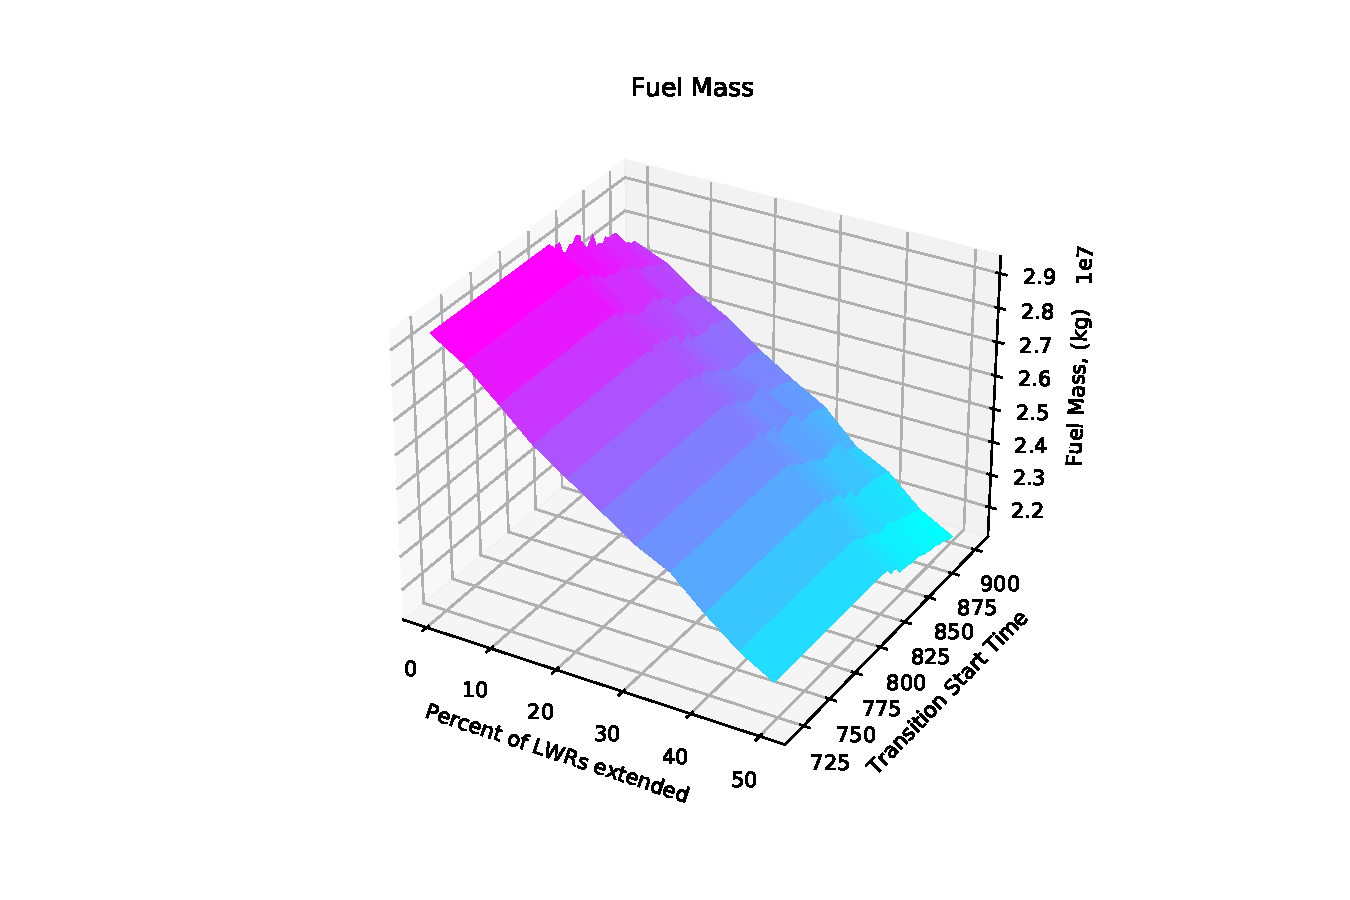
\includegraphics[width=\textwidth, trim=120 0 120 30, clip]{ts_lwr_enr_u.pdf}
        \caption{Effect on total fuel mass.}
        \label{fig:ts_lwr_enr_u}
    \end{subfigure}
    \hfill
    \begin{subfigure}[h!]{0.48\textwidth}
        \centering
        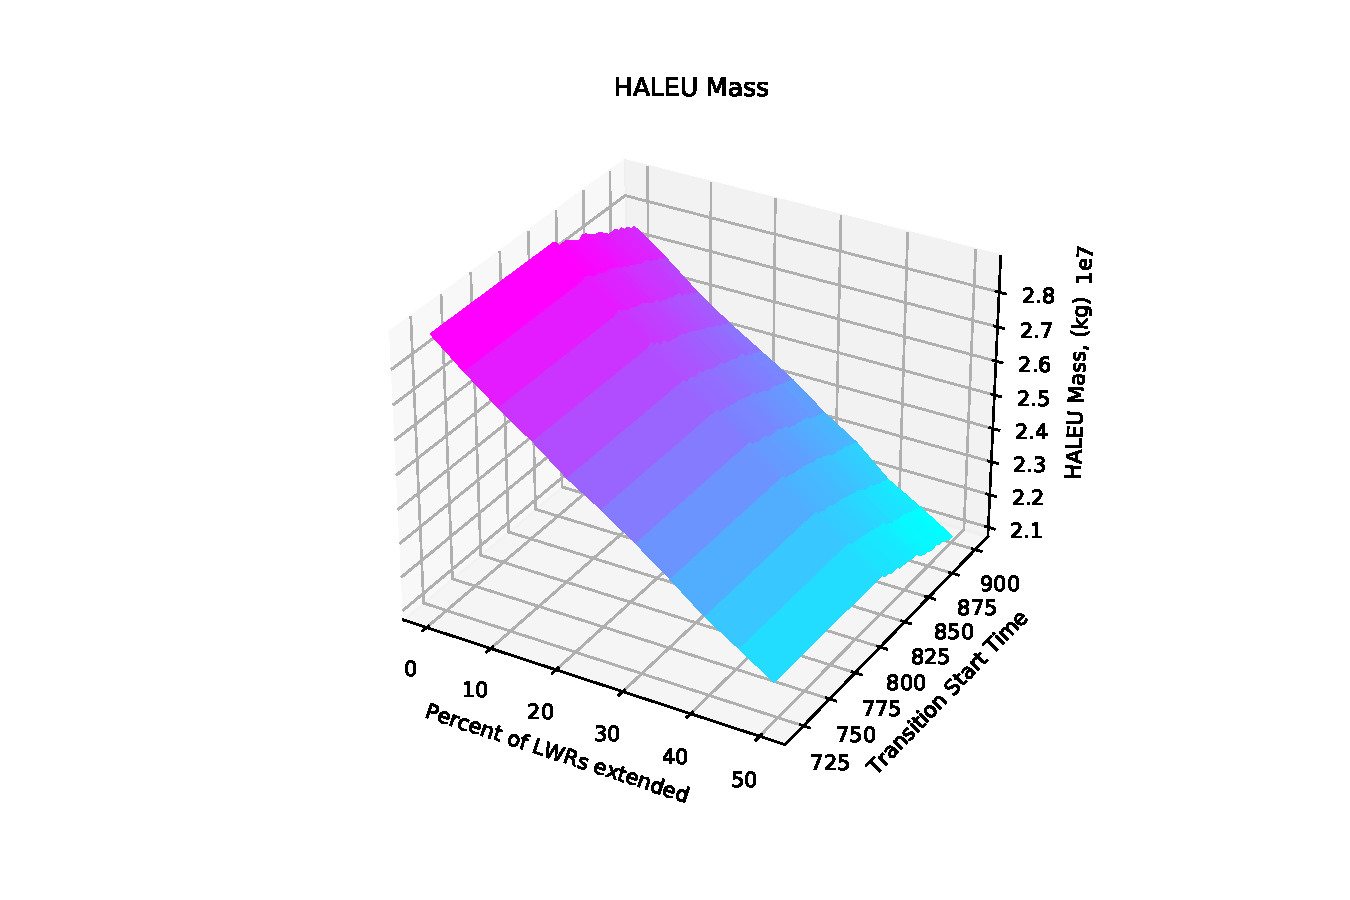
\includegraphics[width=\textwidth, trim=120 0 120 30, clip]{ts_lwr_haleu.pdf}
        \caption{Effect on HALEU mass.}
        \label{fig:ts_lwr_haleu}
    \end{subfigure}
    
    \begin{subfigure}[h!]{0.48\textwidth}
        \centering
        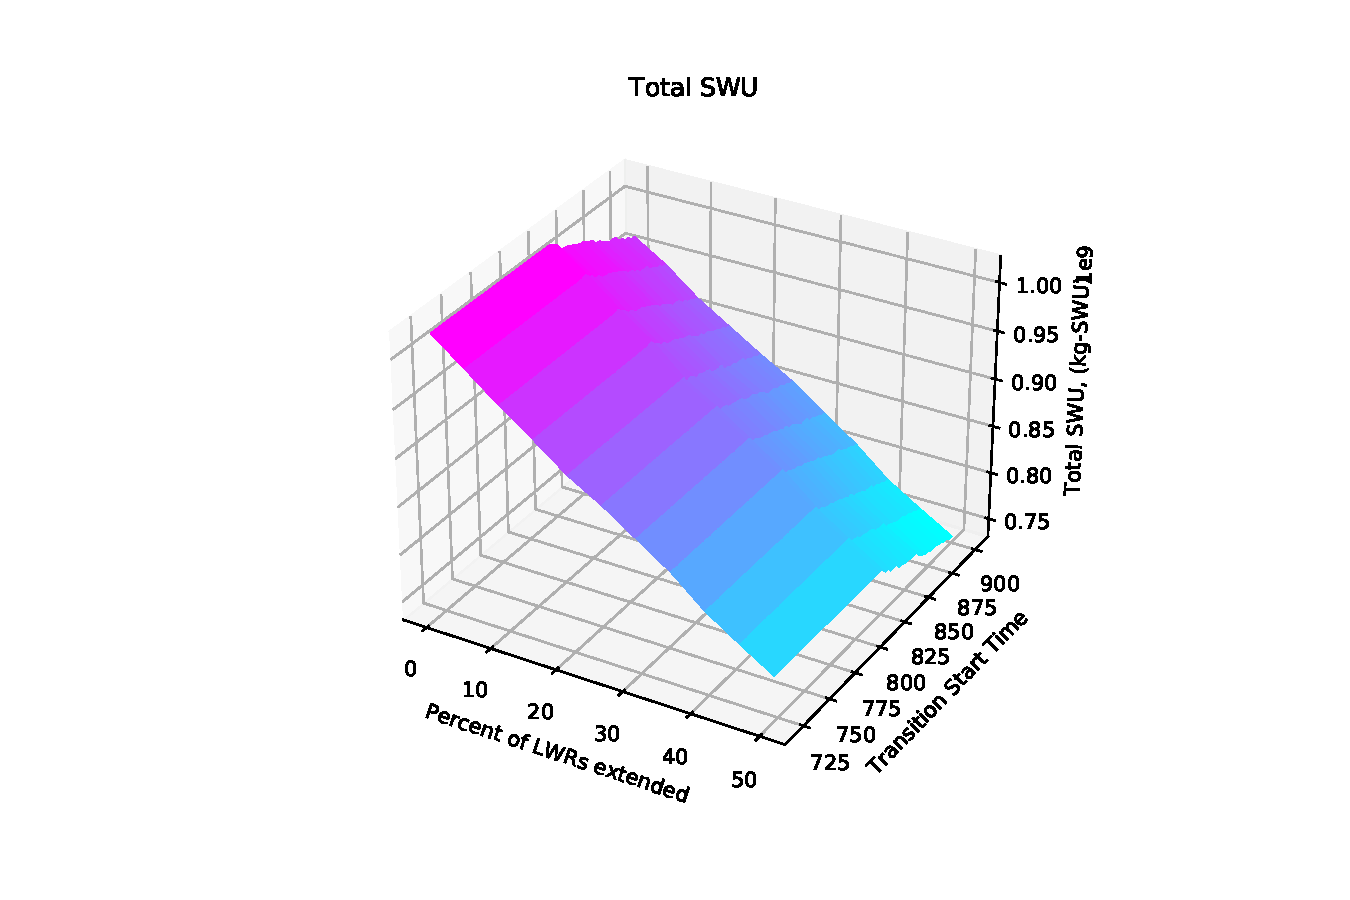
\includegraphics[width=\textwidth, trim=120 0 120 30, clip]{ts_lwr_swu.pdf}
        \caption{Effect on total SWU capacity.}
        \label{fig:ts_lwr_swu}
    \end{subfigure}
    \hfill
    \begin{subfigure}[h!]{0.48\textwidth}
        \centering
        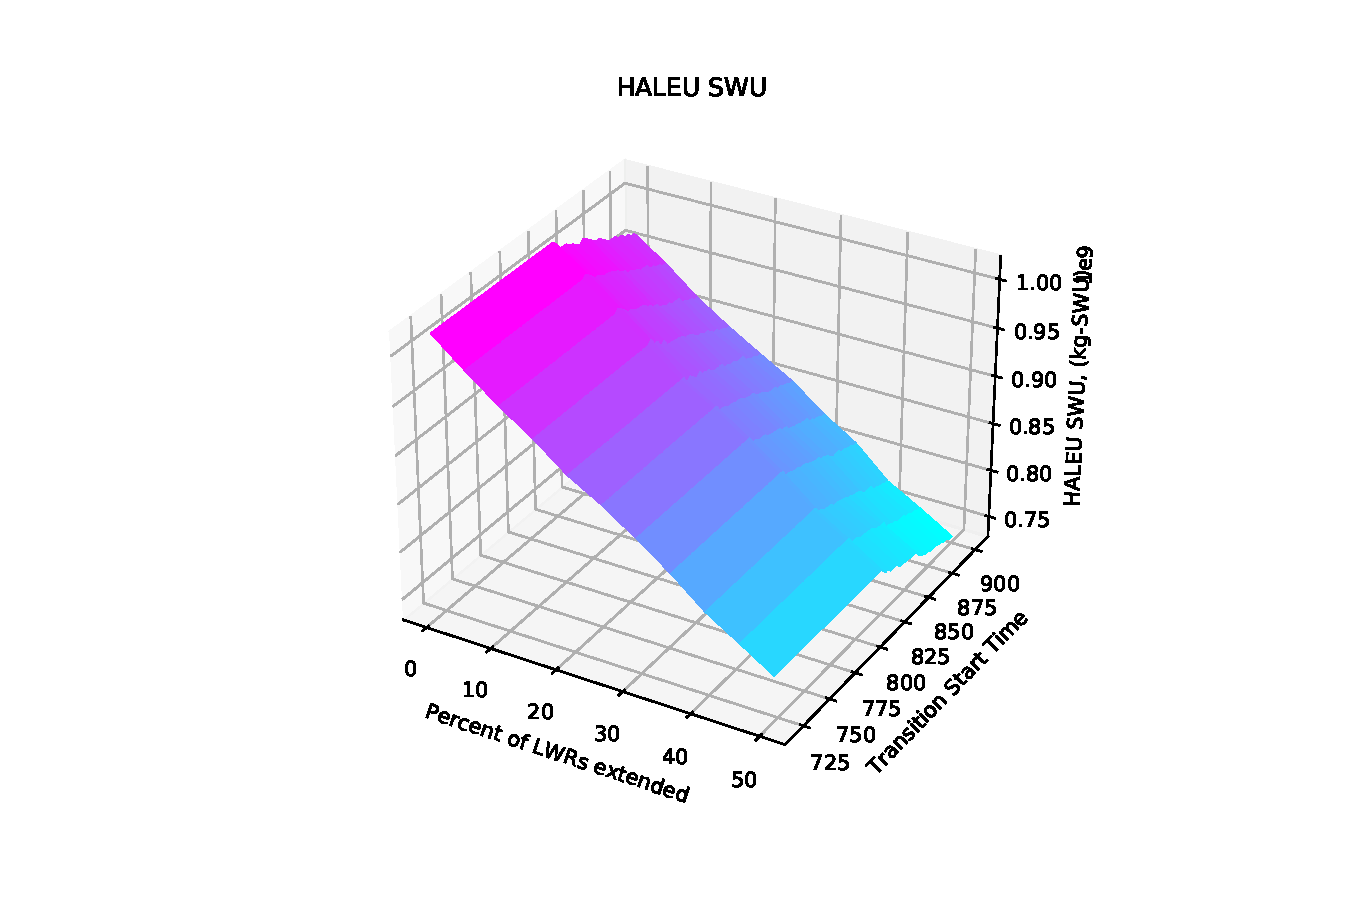
\includegraphics[width=\textwidth, trim=120 0 120 30, clip]{ts_lwr_haleu_swu.pdf}
        \caption{Effect on HALEU SWU capacity.}
        \label{fig:ts_lwr_haleu_swu}
    \end{subfigure}
    \caption{Change in metrics resulting from variations in the 
    transition start time and LWR lifetimes.}
\end{figure}

\begin{figure}
    \ContinuedFloat    
    \begin{subfigure}[h!]{0.48\textwidth}
        \centering
        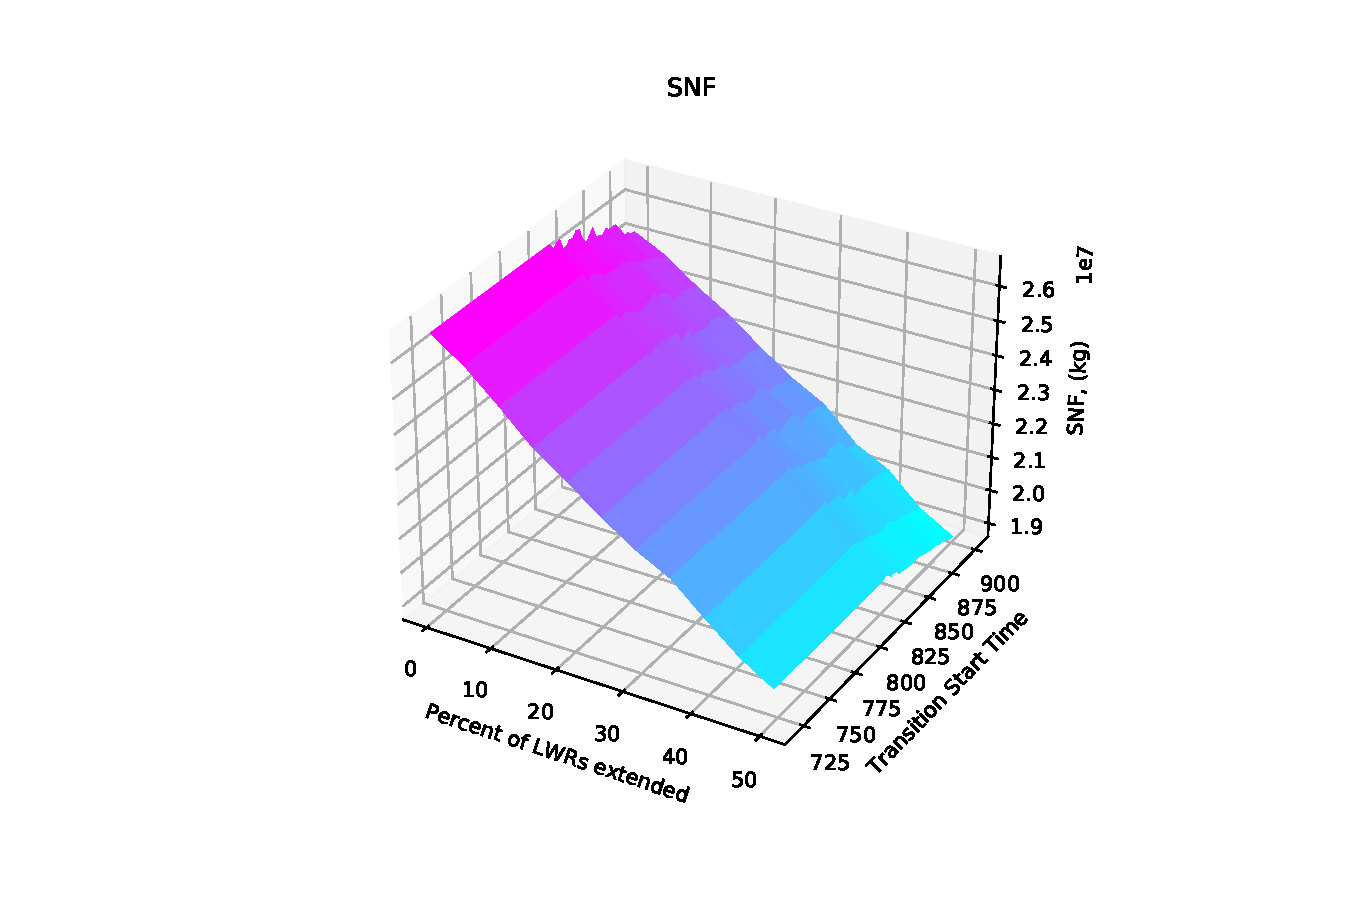
\includegraphics[width=\textwidth, trim=120 0 120 30, clip]{ts_lwr_waste.pdf}
        \caption{Effect on waste mass discharged.}
        \label{fig:ts_lwr_waste}
    \end{subfigure}
    \hfill
    \begin{subfigure}[h!]{0.48\textwidth}
        \centering
        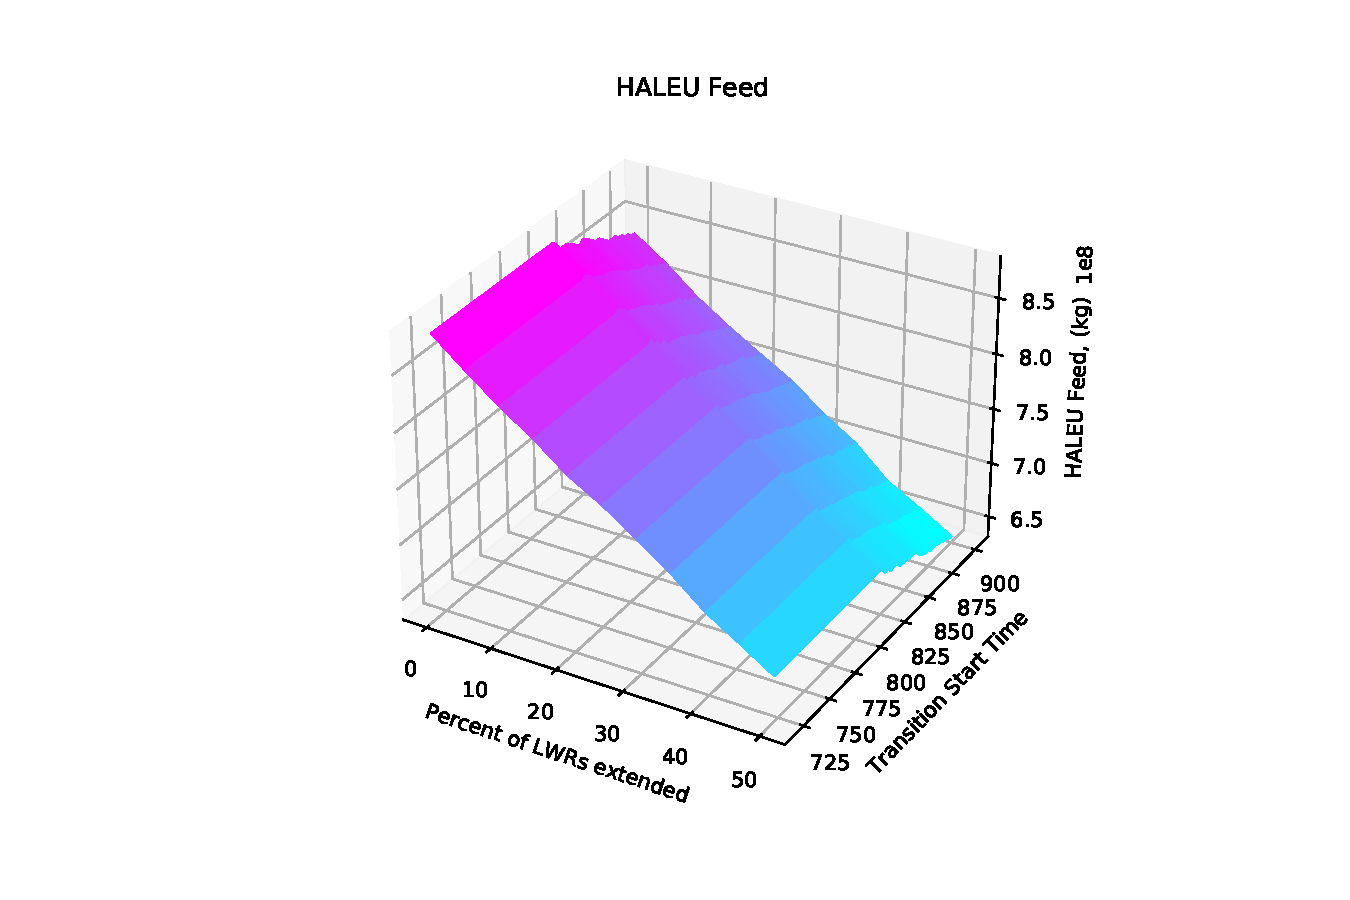
\includegraphics[width=\textwidth, trim=120 0 120 30, clip]{ts_lwr_feed.pdf}
        \caption{Effect on HALEU feed.}
        \label{fig:ts_lwr_feed}
    \end{subfigure}
    \caption{(cont.) Change in metrics resulting from variations in the 
    transition start time and LWR lifetimes.}
    \label{fig:ts_lwr}
\end{figure}

Figure \ref{fig:ts_xe100_share} shows the results of varying the 
transition start time and Xe-100 build share on the \gls{HALEU} mass, 
\gls{SWU} to produce \gls{HALEU}, waste mass discharged, and feed 
to produce \gls{HALEU}. This figure shows that increasing the 
Xe-100 build share has a greater impact on the metrics than 
changing the transition start time, which is consistent with the 
\gls{OAT} results. There is no clear combined effect from varying these 
parameters together. 

\begin{figure}
    \begin{subfigure}[h!]{0.48\textwidth}
        \centering
        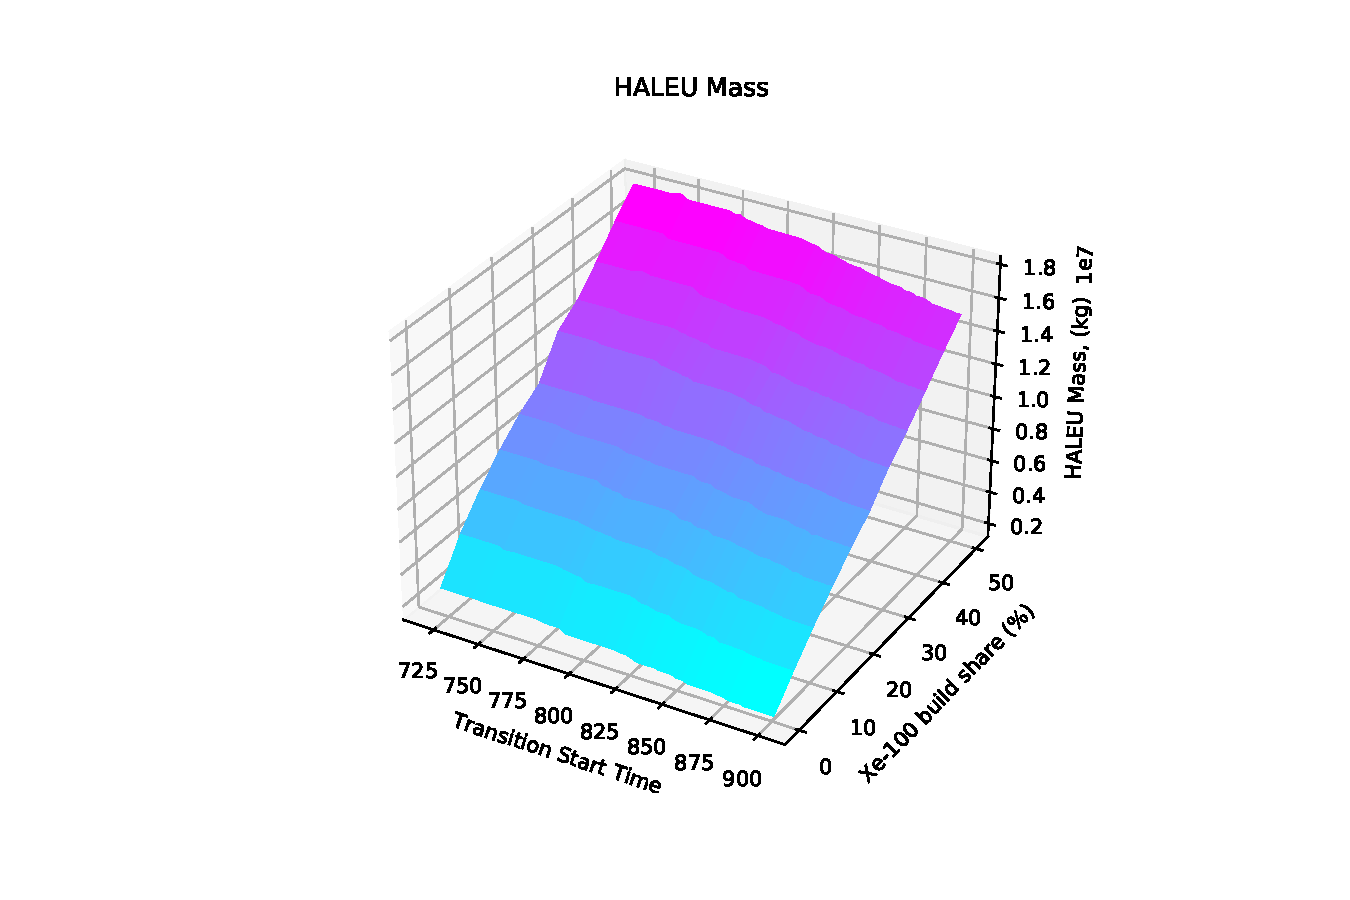
\includegraphics[width=\textwidth, trim=120 0 120 30, clip]{ts_xe100_share_haleu.pdf}
        \caption{Effect on HALEU mass.}
        \label{fig:ts_xe100_share_haleu}
    \end{subfigure}
    \begin{subfigure}[h!]{0.48\textwidth}
        \centering
        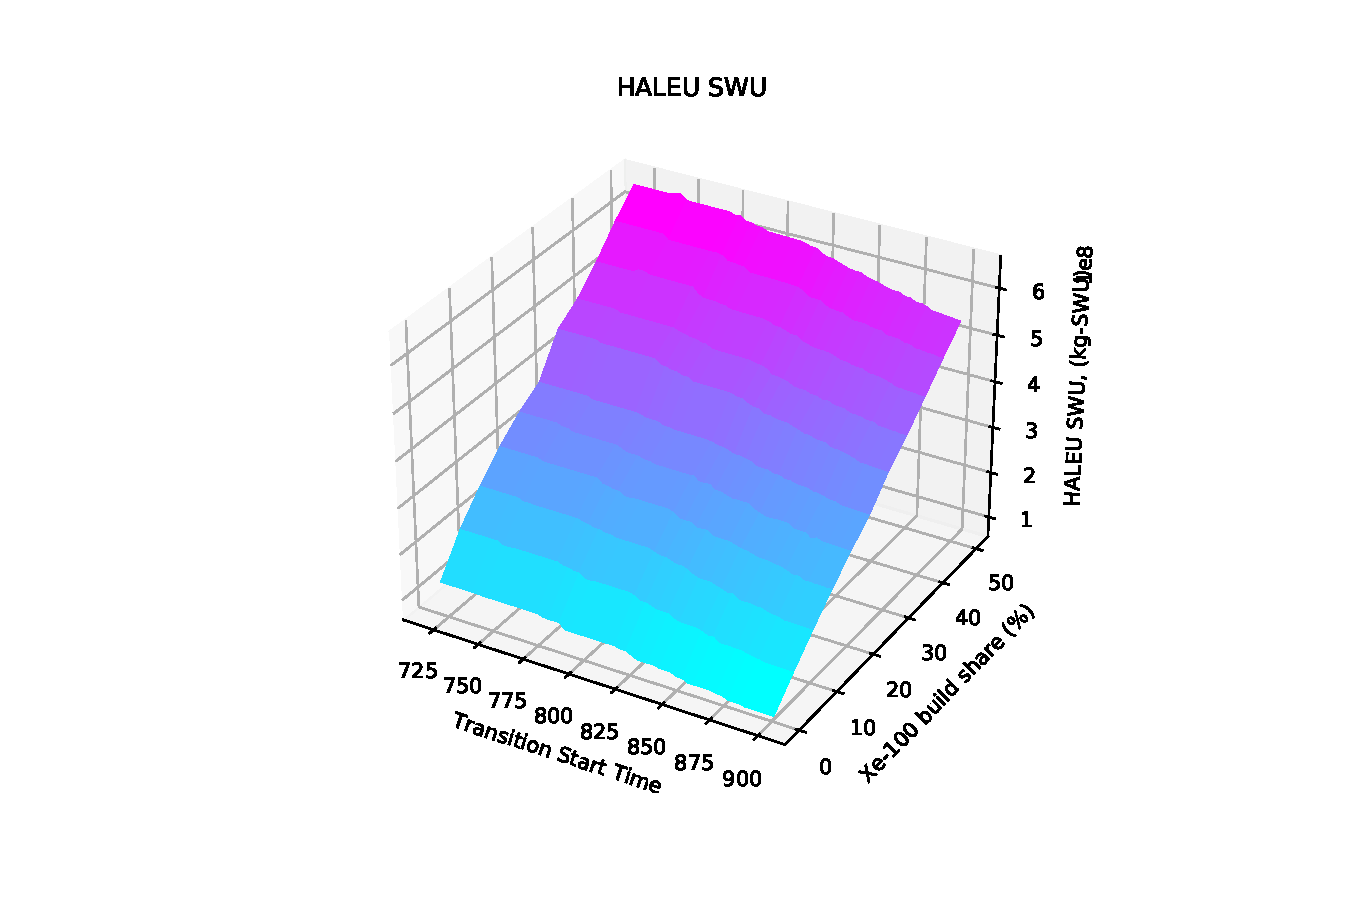
\includegraphics[width=\textwidth, trim=120 0 120 30, clip]{ts_xe100_share_haleu_swu.pdf}
        \caption{Effect on HALEU SWU capacity.}
        \label{fig:ts_xe100_share_haleu_swu}
    \end{subfigure}
    
    \begin{subfigure}[h!]{0.48\textwidth}
        \centering
        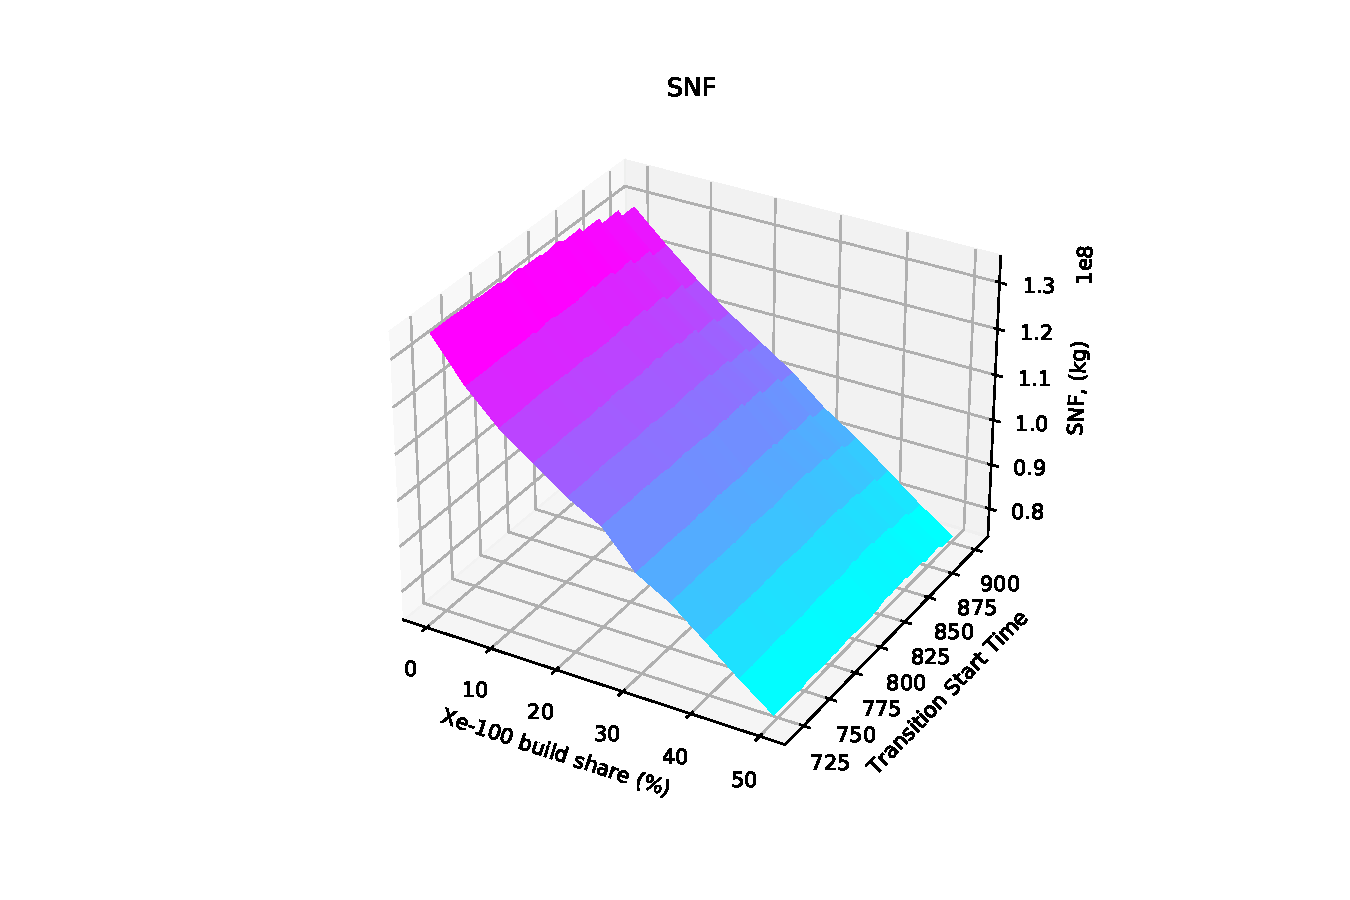
\includegraphics[width=\textwidth, trim=120 0 120 30, clip]{ts_xe100_share_waste.pdf}
        \caption{Effect on waste mass discharged.}
        \label{fig:ts_xe100_share_waste}
    \end{subfigure}
    \hfill
    \begin{subfigure}[h!]{0.48\textwidth}
        \centering
        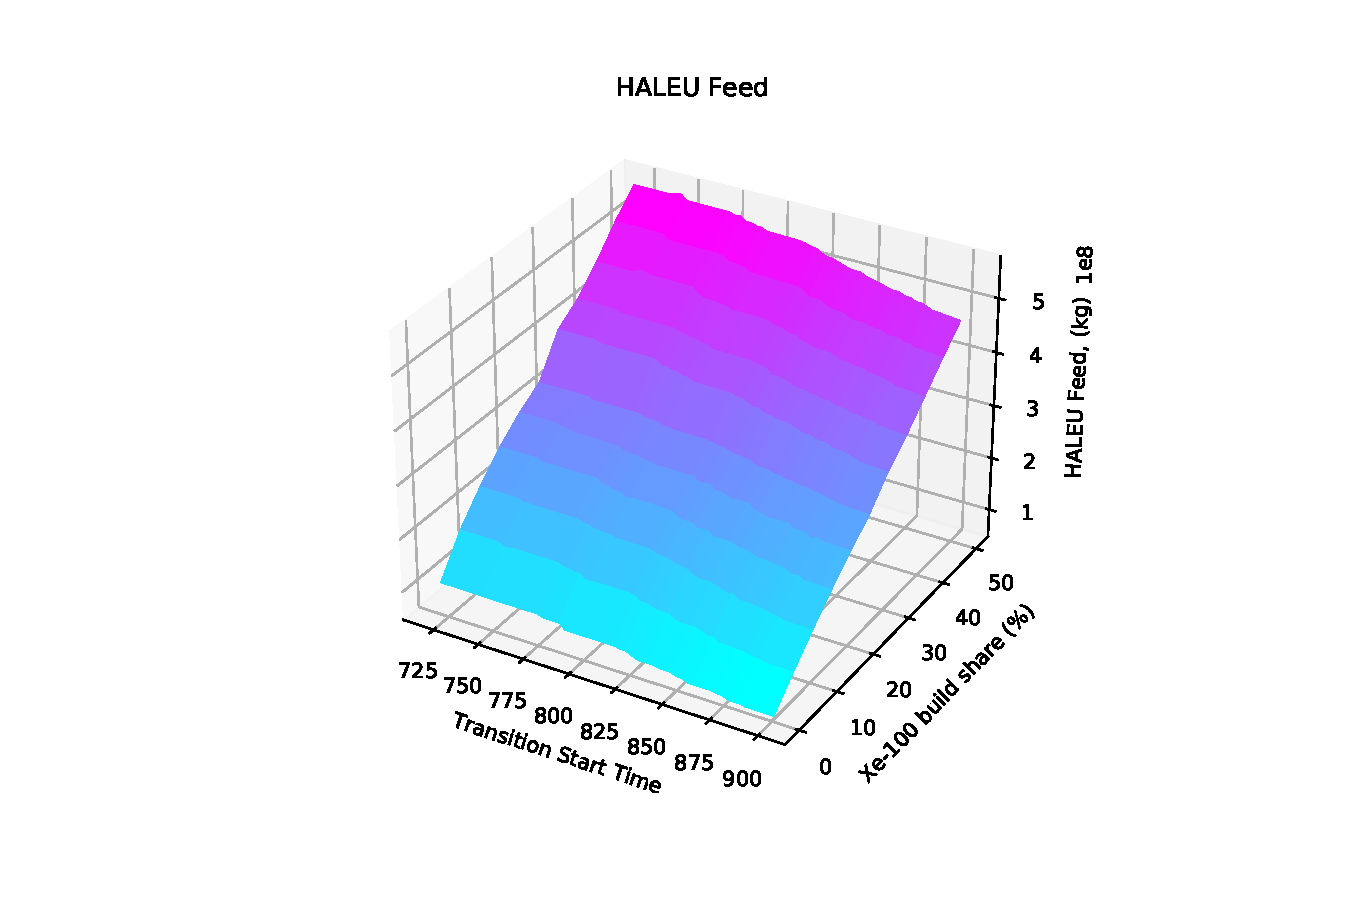
\includegraphics[width=\textwidth, trim=120 0 120 30, clip]{ts_xe100_share_feed.pdf}
        \caption{Effect on HALEU feed.}
        \label{fig:ts_xe100_share_feed}
    \end{subfigure}
    \caption{Change in metrics resulting from variations in the 
    transition start time and Xe-100 build share.}
    \label{fig:ts_xe100_share}
\end{figure}

Figure \ref{fig:ts_mmr_share} shows the results of varying the 
transition start time and the \gls{MMR} build share on all 
six of the metrics. The \gls{HALEU}-related metrics and the total 
\gls{SWU} capacity show a much stronger effect from the \gls{MMR} 
build share than the transition start time. The total fuel mass 
and \gls{UNF} mass show an effect from varying both parameters, 
but they do not compound on each other (result in a non-linear 
trend in the metric). 

\begin{figure}
    \begin{subfigure}[h!]{0.48\textwidth}
        \centering
        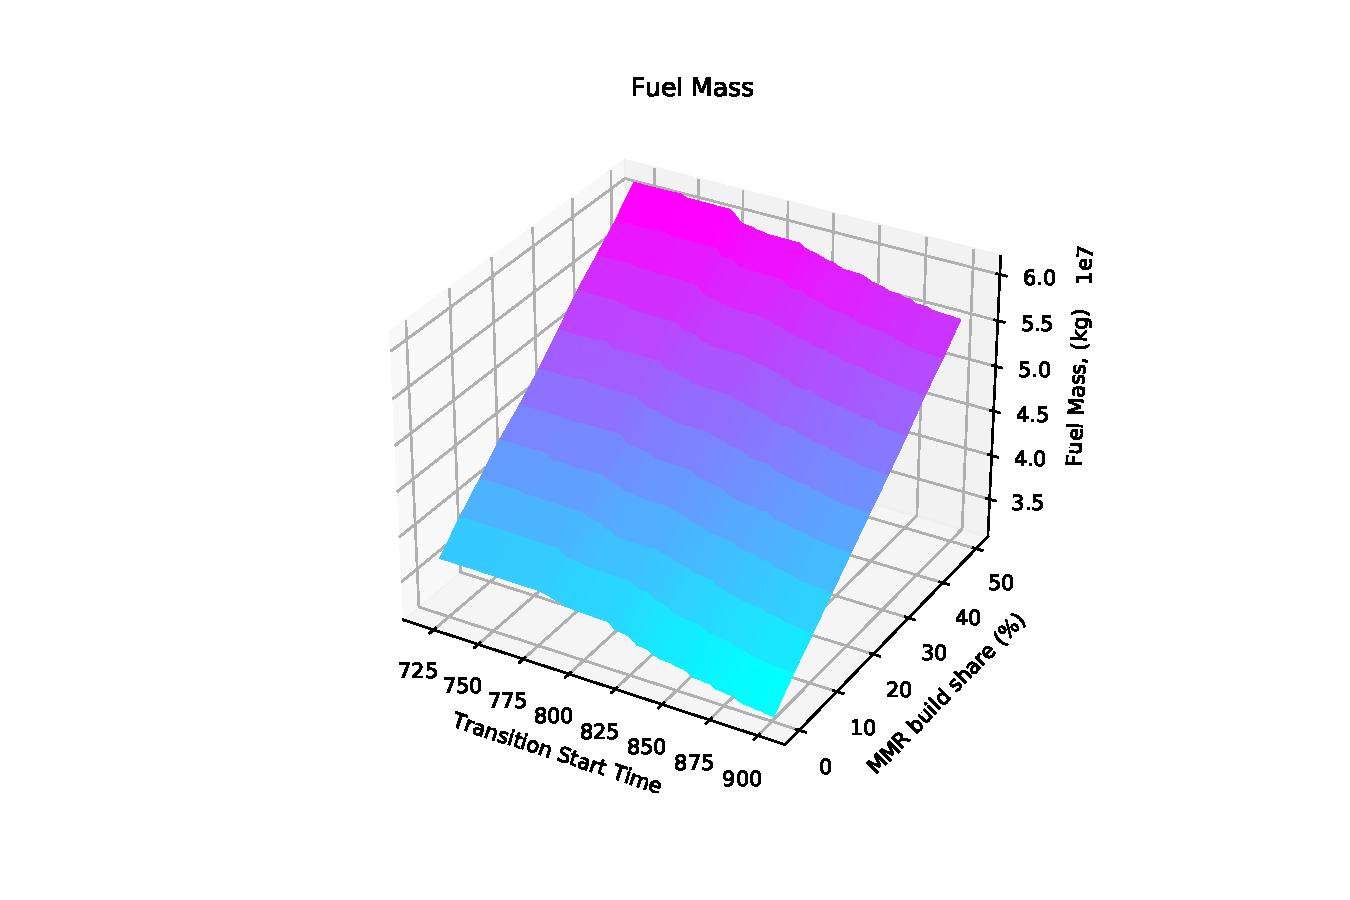
\includegraphics[width=\textwidth, trim=120 0 120 30, clip]{ts_mmr_share_enr_u.pdf}
        \caption{Effect on total fuel mass.}
        \label{fig:ts_mmr_share_enr_u}
    \end{subfigure}
    \hfill
    \begin{subfigure}[h!]{0.48\textwidth}
        \centering
        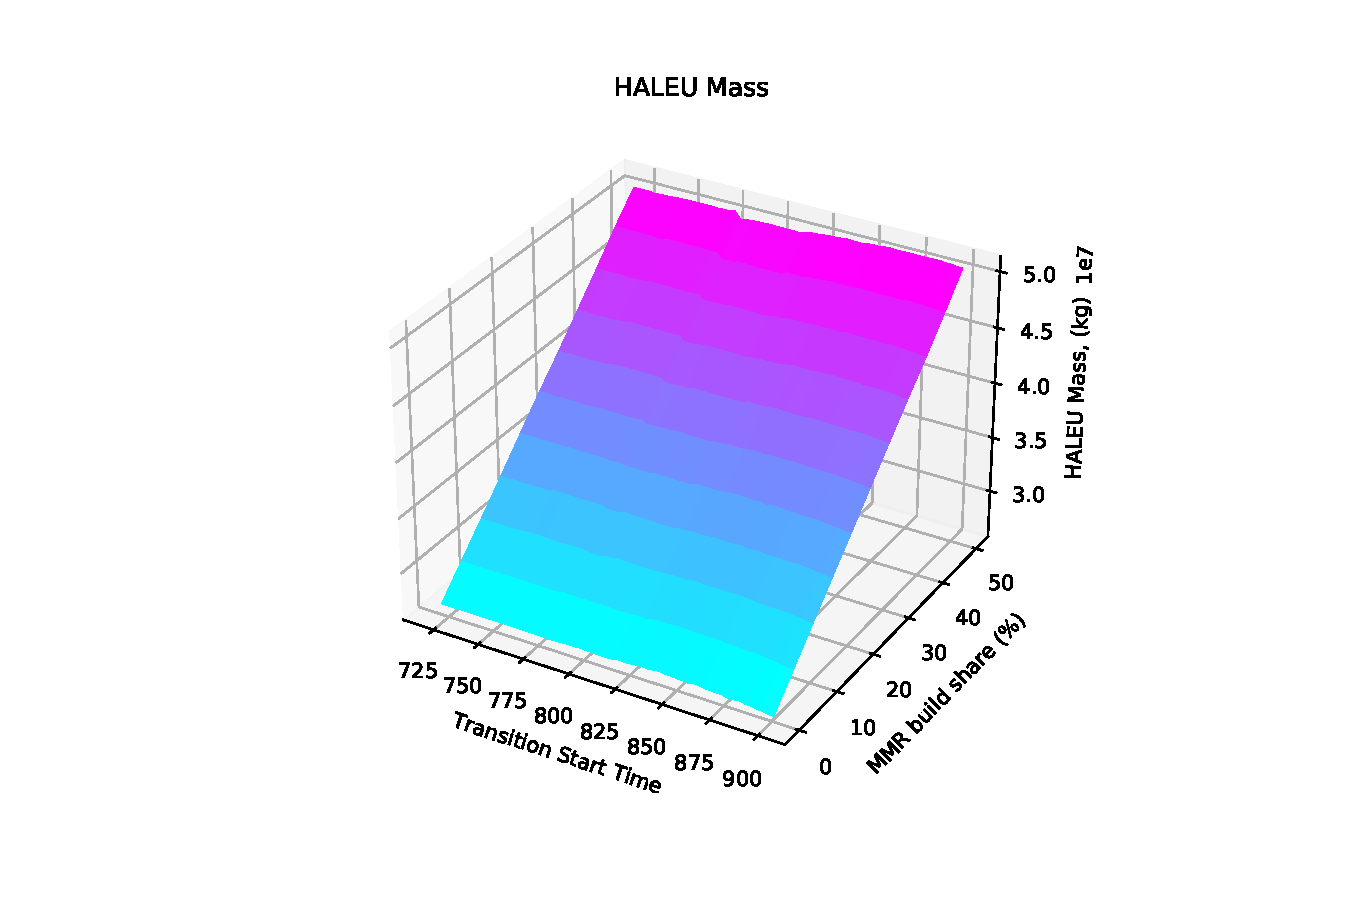
\includegraphics[width=\textwidth, trim=120 0 120 30, clip]{ts_mmr_share_haleu.pdf}
        \caption{Effect on HALEU mass.}
        \label{fig:ts_mmr_share_haleu}
    \end{subfigure}
    
    \begin{subfigure}[h!]{0.48\textwidth}
        \centering
        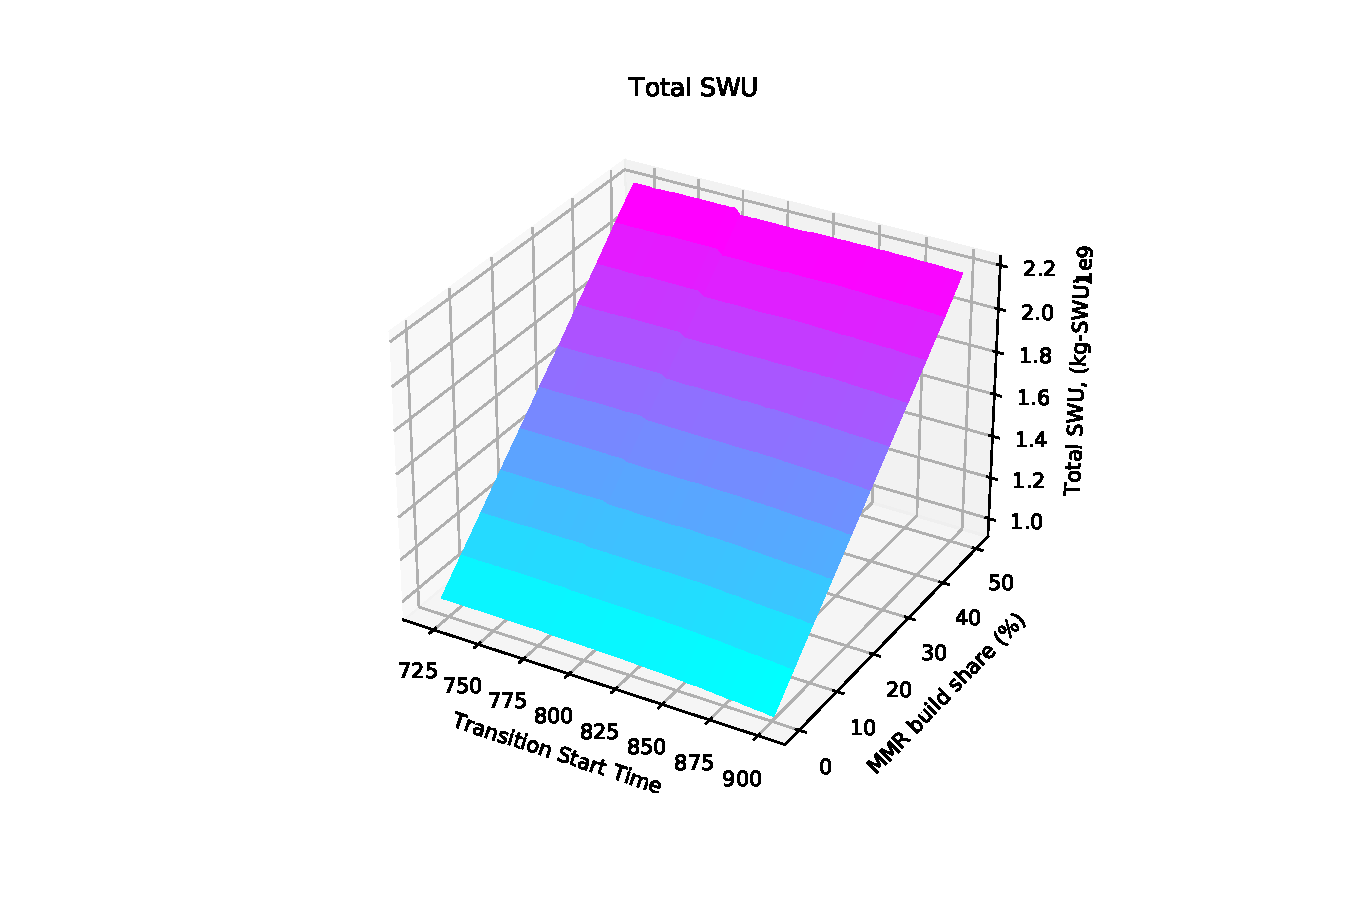
\includegraphics[width=\textwidth, trim=120 0 120 30, clip]{ts_mmr_share_swu.pdf}
        \caption{Effect on total SWU capacity.}
        \label{fig:ts_mmr_share_swu}
    \end{subfigure}
    \hfill
    \begin{subfigure}[h!]{0.48\textwidth}
        \centering
        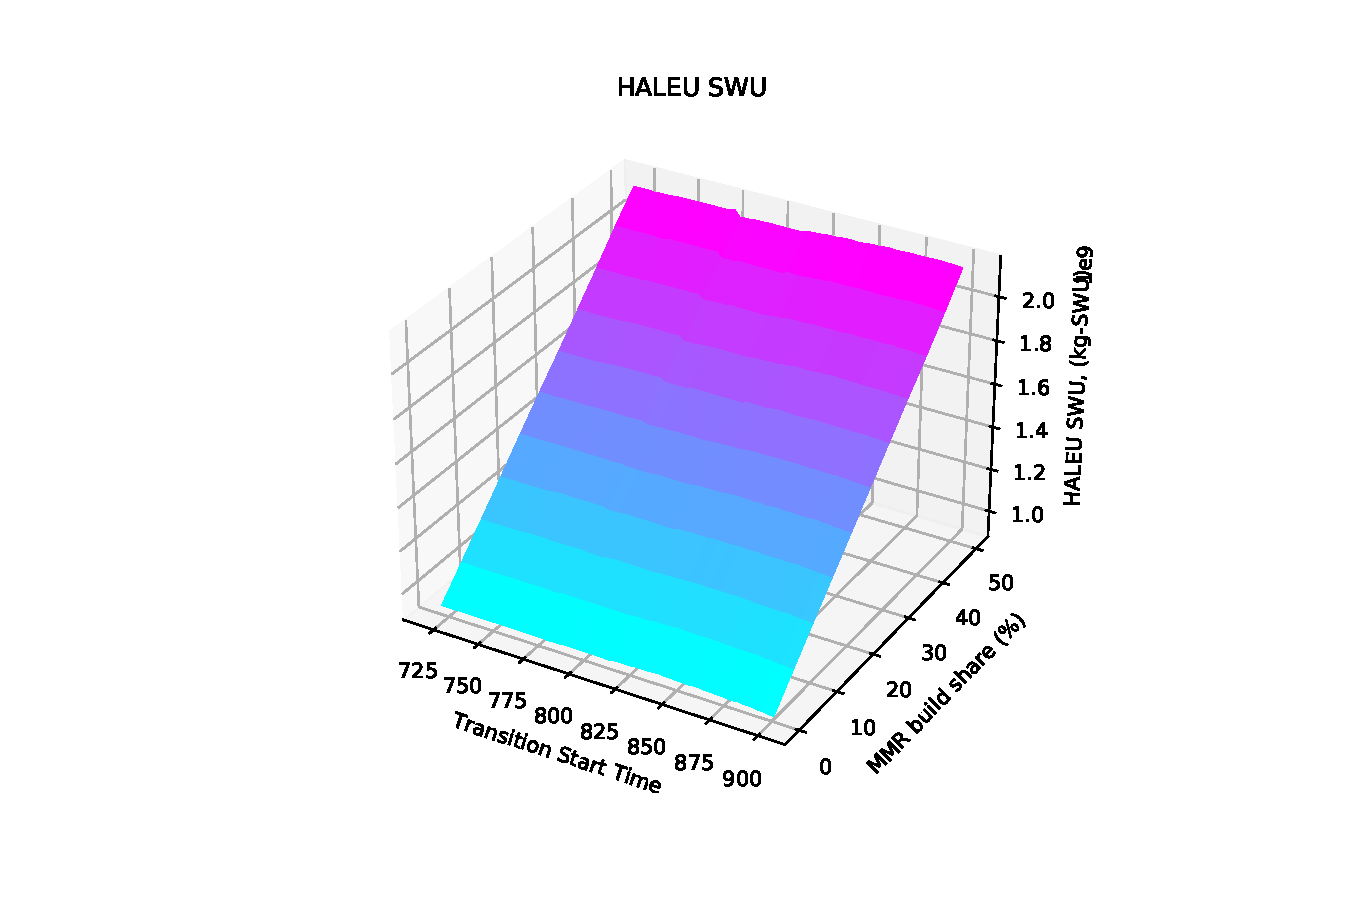
\includegraphics[width=\textwidth, trim=120 0 120 30, clip]{ts_mmr_share_haleu_swu.pdf}
        \caption{Effect on HALEU SWU capacity.}
        \label{fig:ts_mmr_share_haleu_swu}
    \end{subfigure}
    \caption{Change in metrics resulting from variations in the 
    transition start time and MMR build share.}
\end{figure}

\begin{figure}
    \ContinuedFloat
    \begin{subfigure}[h!]{0.48\textwidth}
        \centering
        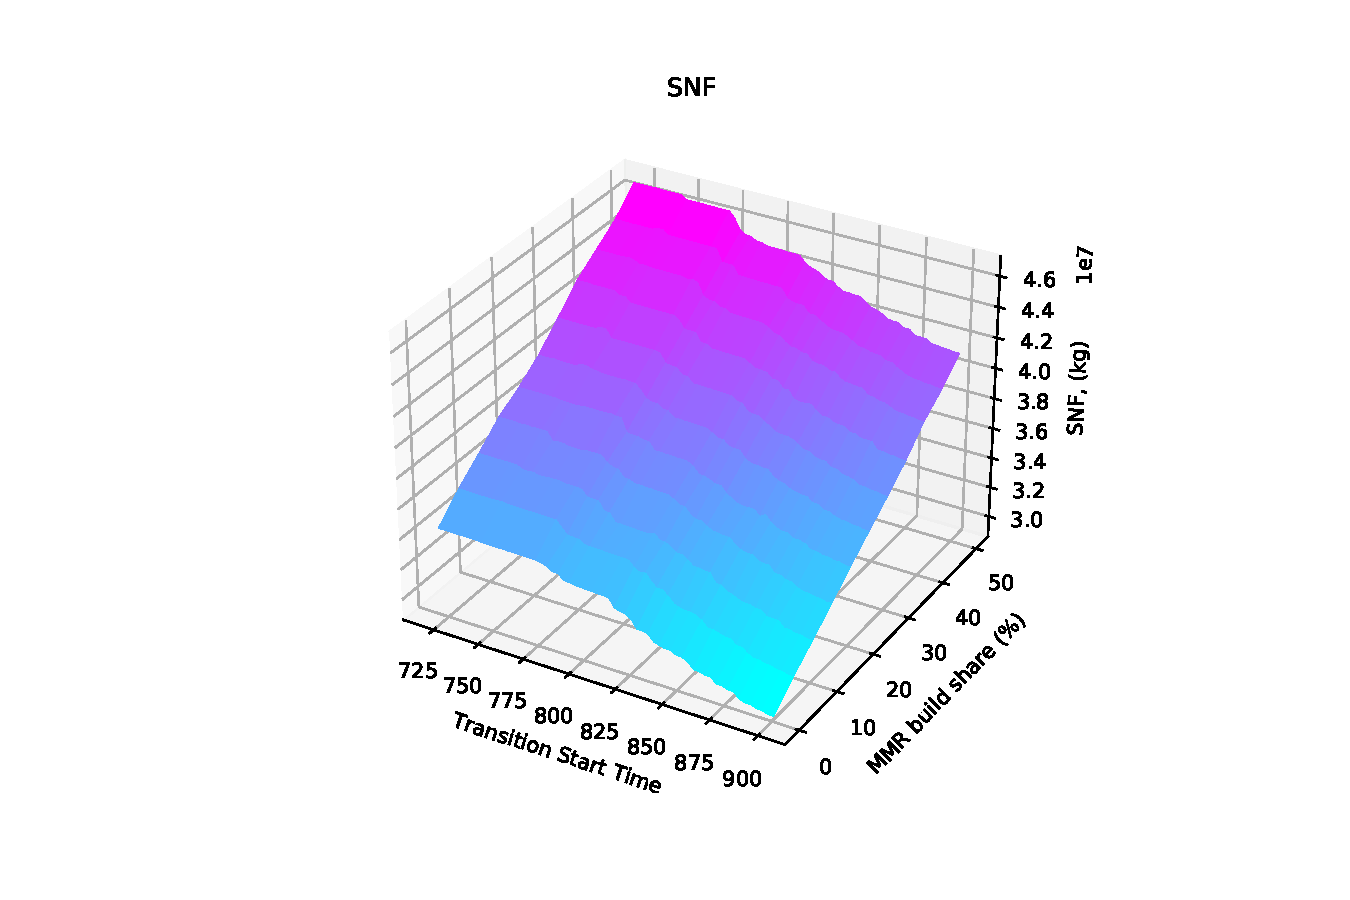
\includegraphics[width=\textwidth, trim=120 0 120 30, clip]{ts_mmr_share_waste.pdf}
        \caption{Effect on waste mass discharged.}
        \label{fig:ts_mmr_share_waste}
    \end{subfigure}
    \hfill
    \begin{subfigure}[h!]{0.48\textwidth}
        \centering
        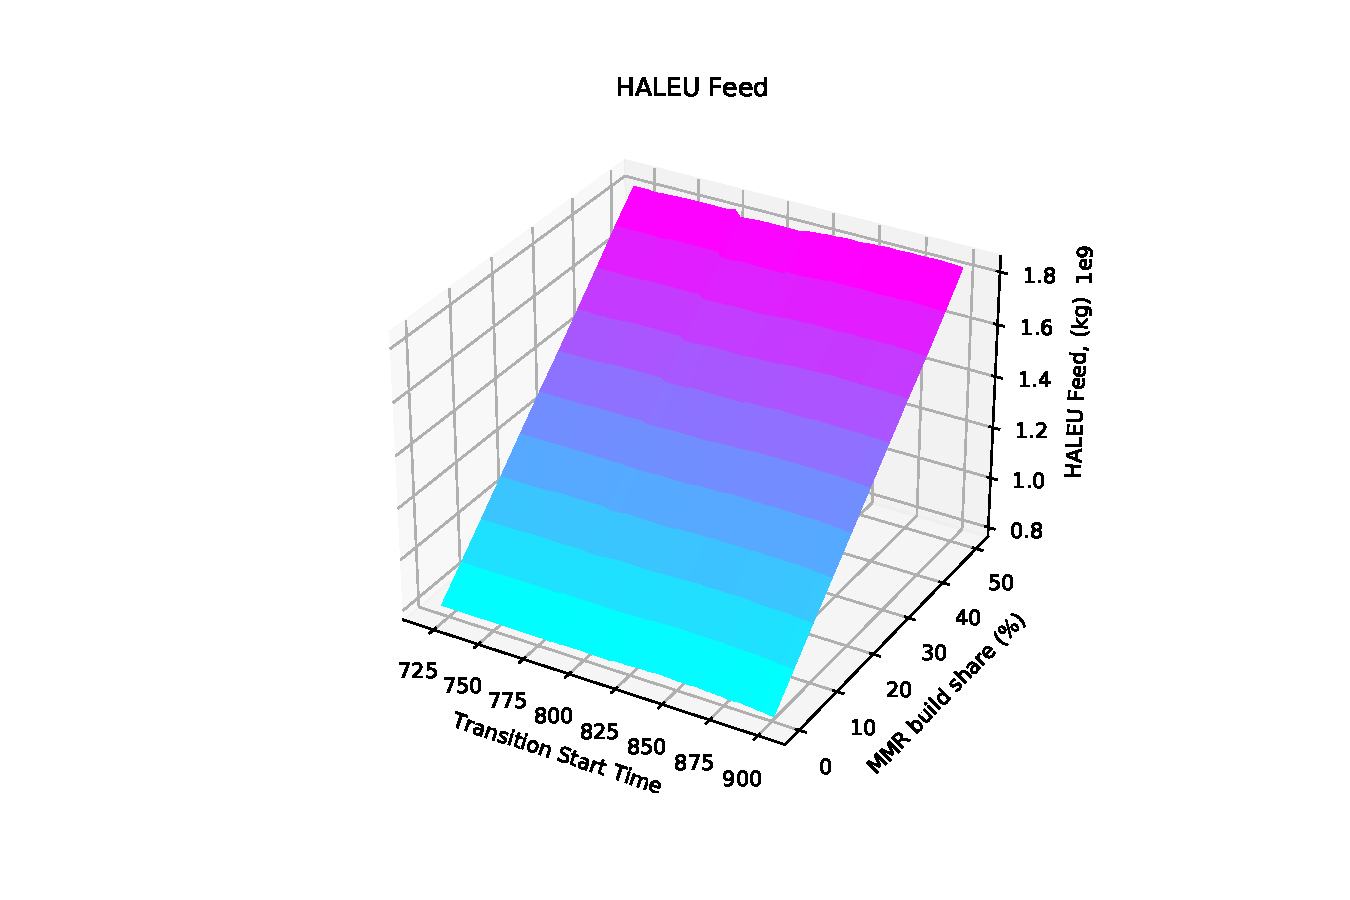
\includegraphics[width=\textwidth, trim=120 0 120 30, clip]{ts_mmr_share_feed.pdf}
        \caption{Effect on HALEU feed.}
        \label{fig:ts_mmr_share_feed}
    \end{subfigure}
    \caption{(cont.) Change in metrics resulting from variations in the 
    transition start time and MMR build share.}
    \label{fig:ts_mmr_share}
\end{figure}

Figure \ref{fig:ts_voygr_share} shows the effects of varying the 
transition start time and the VOYGR build share on all six of the 
metrics. Except for the total \gls{SWU} capacity, the metrics 
exhibit more impact from the VOYGR build share than the 
transition start time. The total \gls{SWU} capacity is impacted more 
by the transition start time than the VOYGR build share. This
different trend is because the Xe-100 and VOYGR require similar 
\gls{SWU} capacity, so this parameter has almost no impact on 
this metric. 

\begin{figure}
    \begin{subfigure}[h!]{0.48\textwidth}
        \centering
        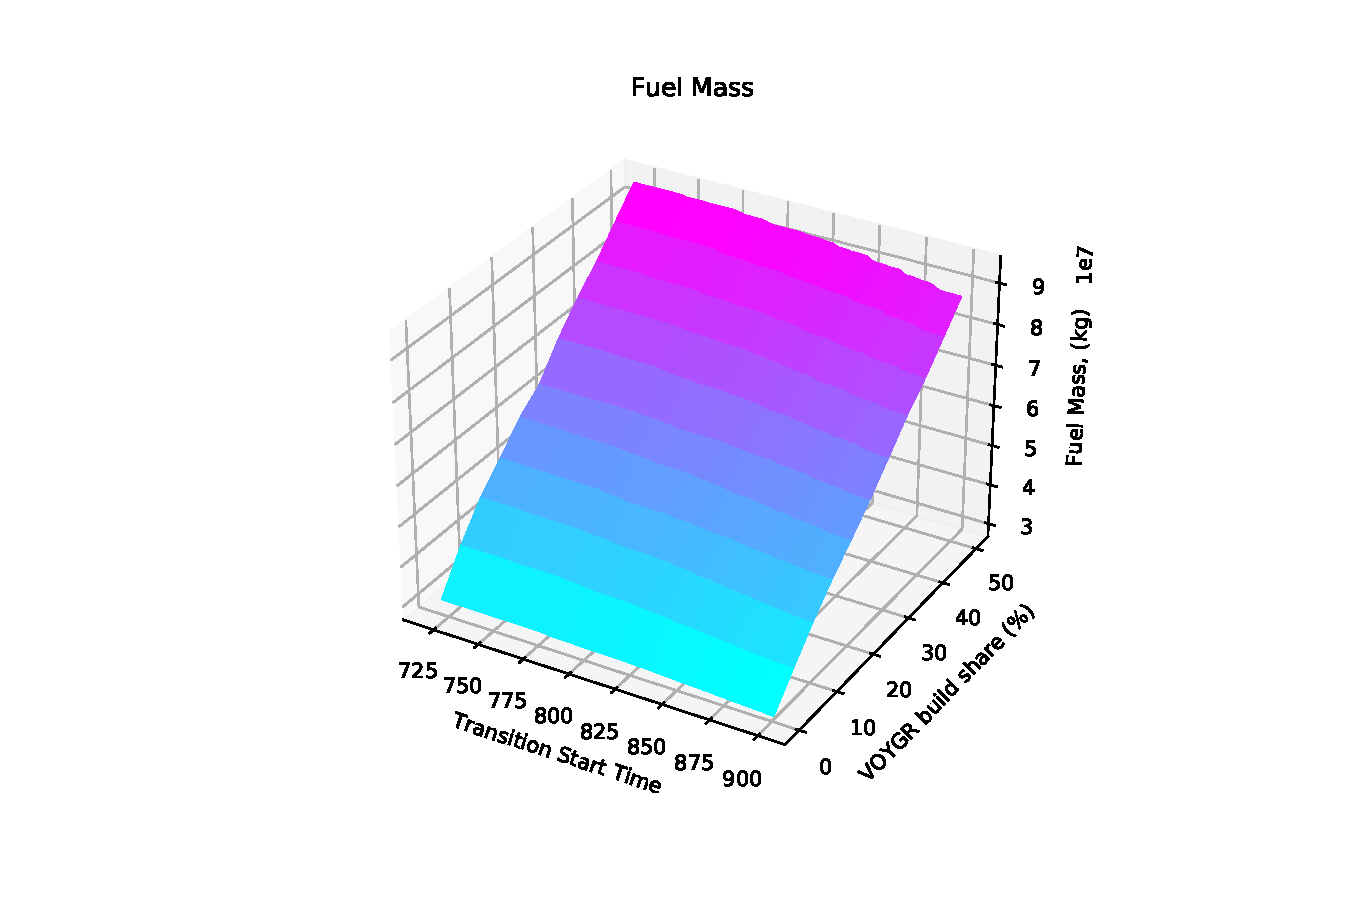
\includegraphics[width=\textwidth, trim=120 0 120 30, clip]{ts_voygr_share_enr_u.pdf}
        \caption{Effect on total fuel mass.}
        \label{fig:ts_voygr_share_enr_u}
    \end{subfigure}
    \hfill
    \begin{subfigure}[h!]{0.48\textwidth}
        \centering
        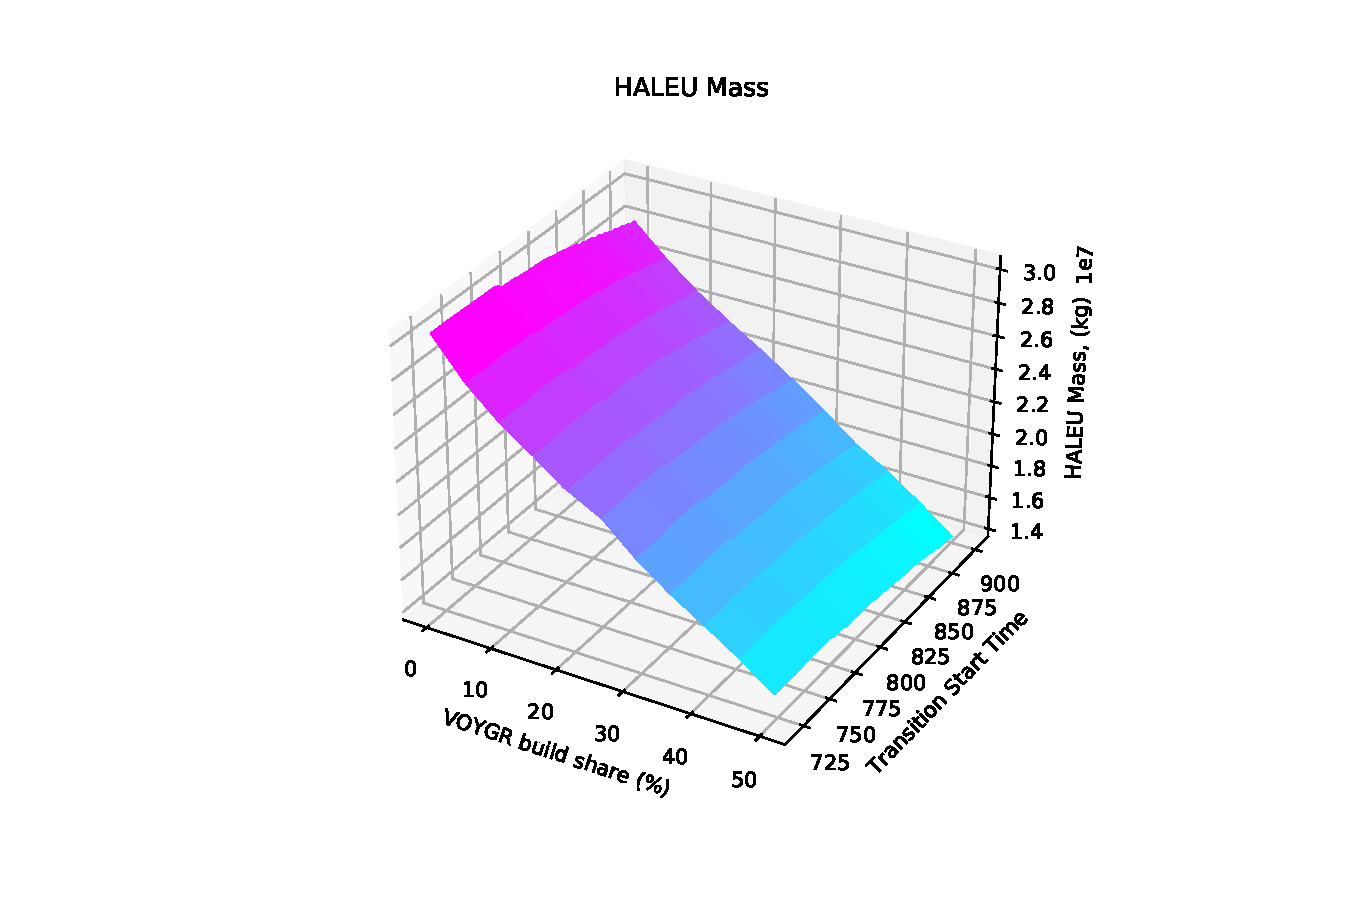
\includegraphics[width=\textwidth, trim=120 0 120 30, clip]{ts_voygr_share_haleu.pdf}
        \caption{Effect on HALEU mass.}
        \label{fig:ts_voygr_share_haleu}
    \end{subfigure}
    \caption{Change in metrics resulting from variations in the 
    transition start time and VOYGR build share.}
\end{figure}

\begin{figure}
    \ContinuedFloat
    \begin{subfigure}[h!]{0.48\textwidth}
        \centering
        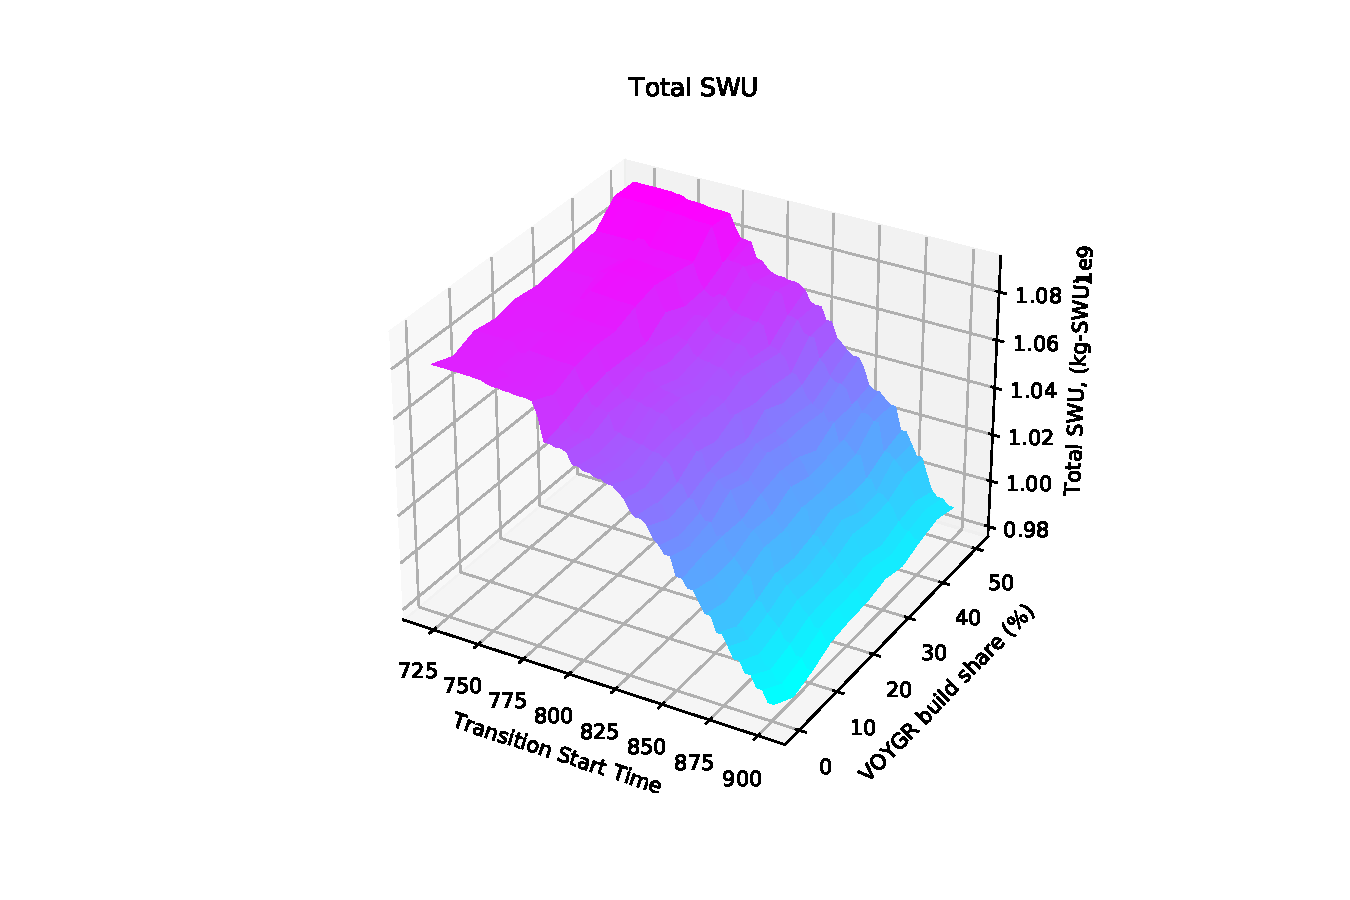
\includegraphics[width=\textwidth, trim=120 0 120 30, clip]{ts_voygr_share_swu.pdf}
        \caption{Effect on total SWU capacity.}
        \label{fig:ts_voygr_share_swu}
    \end{subfigure}
    \hfill
    \begin{subfigure}[h!]{0.48\textwidth}
        \centering
        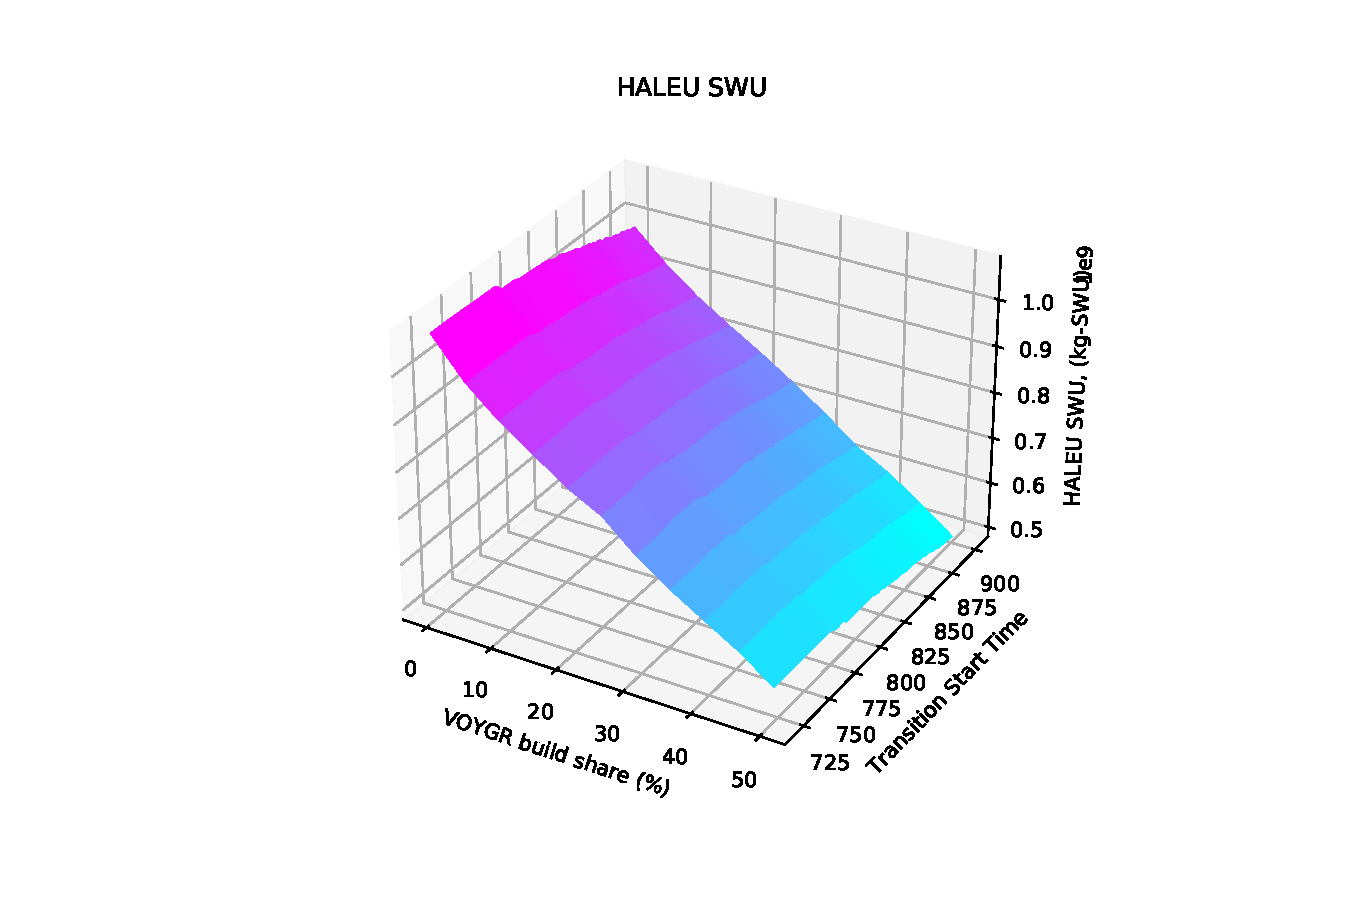
\includegraphics[width=\textwidth, trim=120 0 120 30, clip]{ts_voygr_share_haleu_swu.pdf}
        \caption{Effect on HALEU SWU capacity.}
        \label{fig:ts_voygr_share_haleu_swu}
    \end{subfigure}
    
    \begin{subfigure}[h!]{0.48\textwidth}
        \centering
        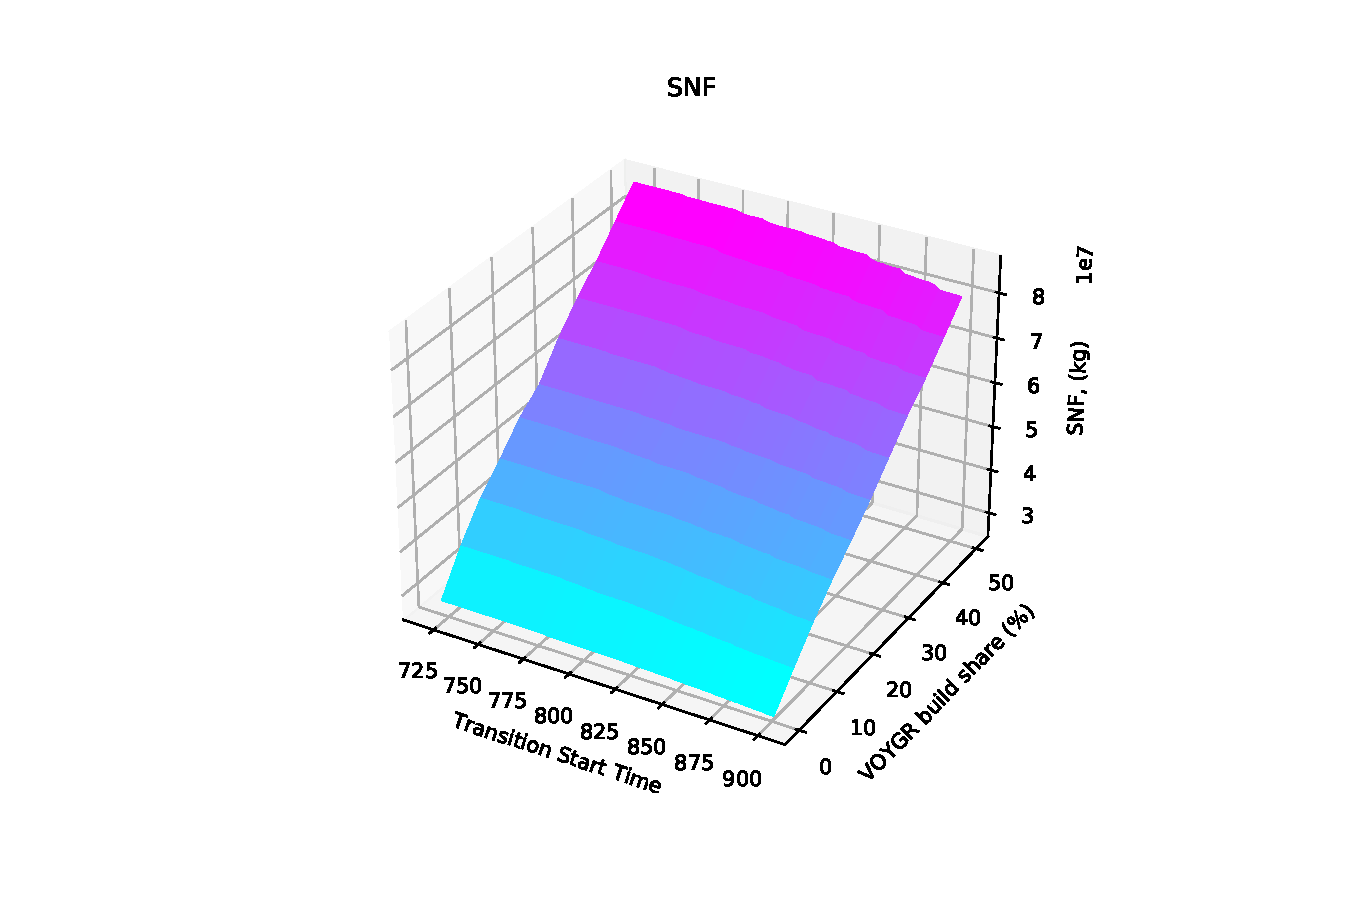
\includegraphics[width=\textwidth, trim=120 0 120 30, clip]{ts_voygr_share_waste.pdf}
        \caption{Effect on waste mass discharged.}
        \label{fig:ts_voygr_share_waste}
    \end{subfigure}
    \hfill
    \begin{subfigure}[h!]{0.48\textwidth}
        \centering
        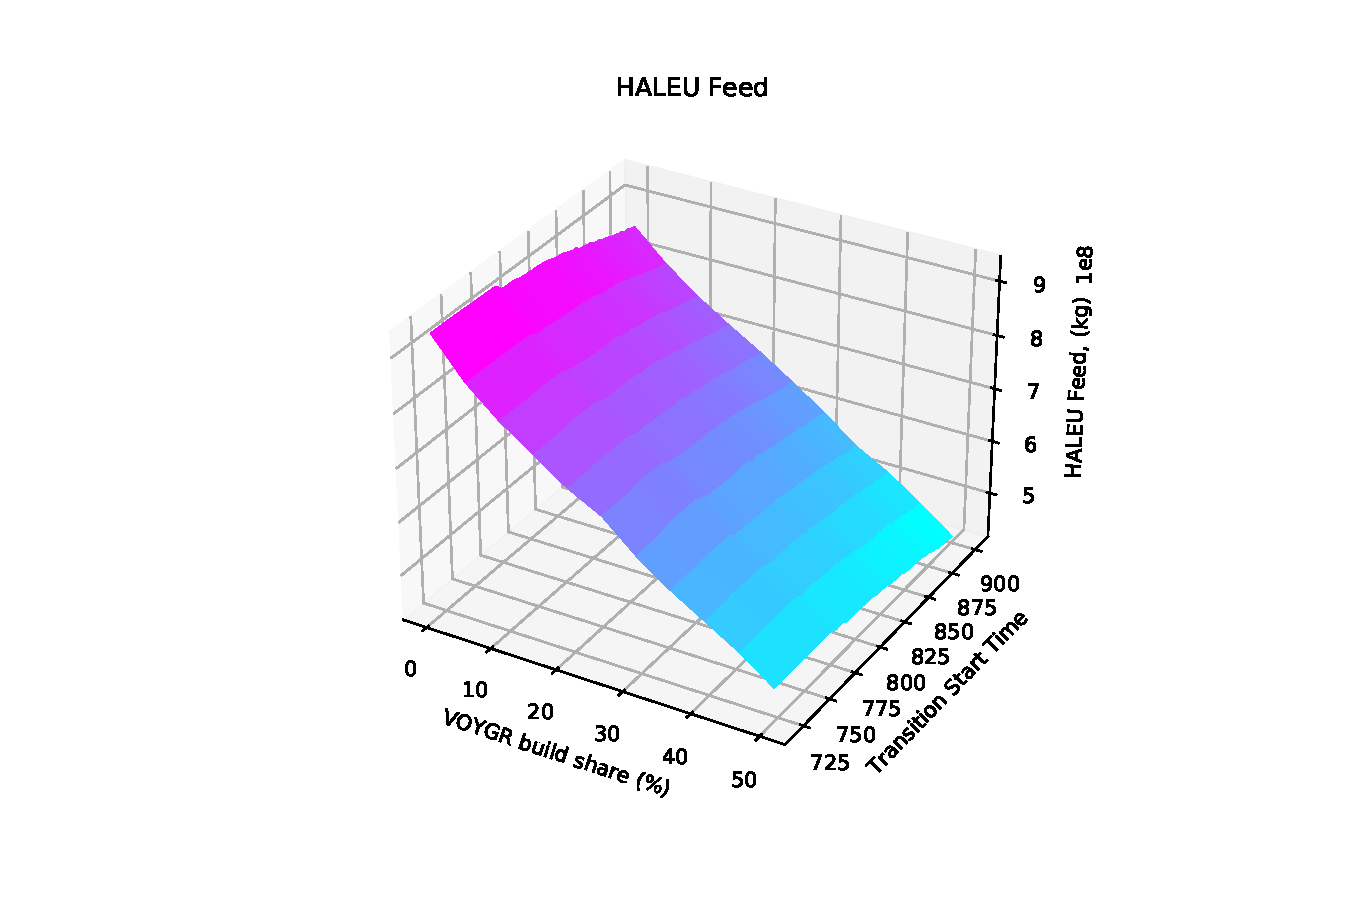
\includegraphics[width=\textwidth, trim=120 0 120 30, clip]{ts_voygr_share_feed.pdf}
        \caption{Effect on HALEU feed.}
        \label{fig:ts_voygr_share_feed}
    \end{subfigure}
    \caption{(cont.) Change in metrics resulting from variations in the 
    transition start time and VOYGR build share.}
    \label{fig:ts_voygr_share}
\end{figure}

Figure \ref{fig:ts_xe100_bu} shows the effects of varying the 
transition start time and the Xe-100 discharge burnup on all six 
metrics. These two parameters impact all six of the metrics in 
a similar matter: the metrics decrease as the Xe-100 burnup increases 
and are not greatly impacted by the transition start time. The 
Xe-100 burnup has a more pronounced effect on the metrics because Xe-100s 
comprise most of the advanced reactors. 

\begin{figure}
    \begin{subfigure}[h!]{0.48\textwidth}
        \centering
        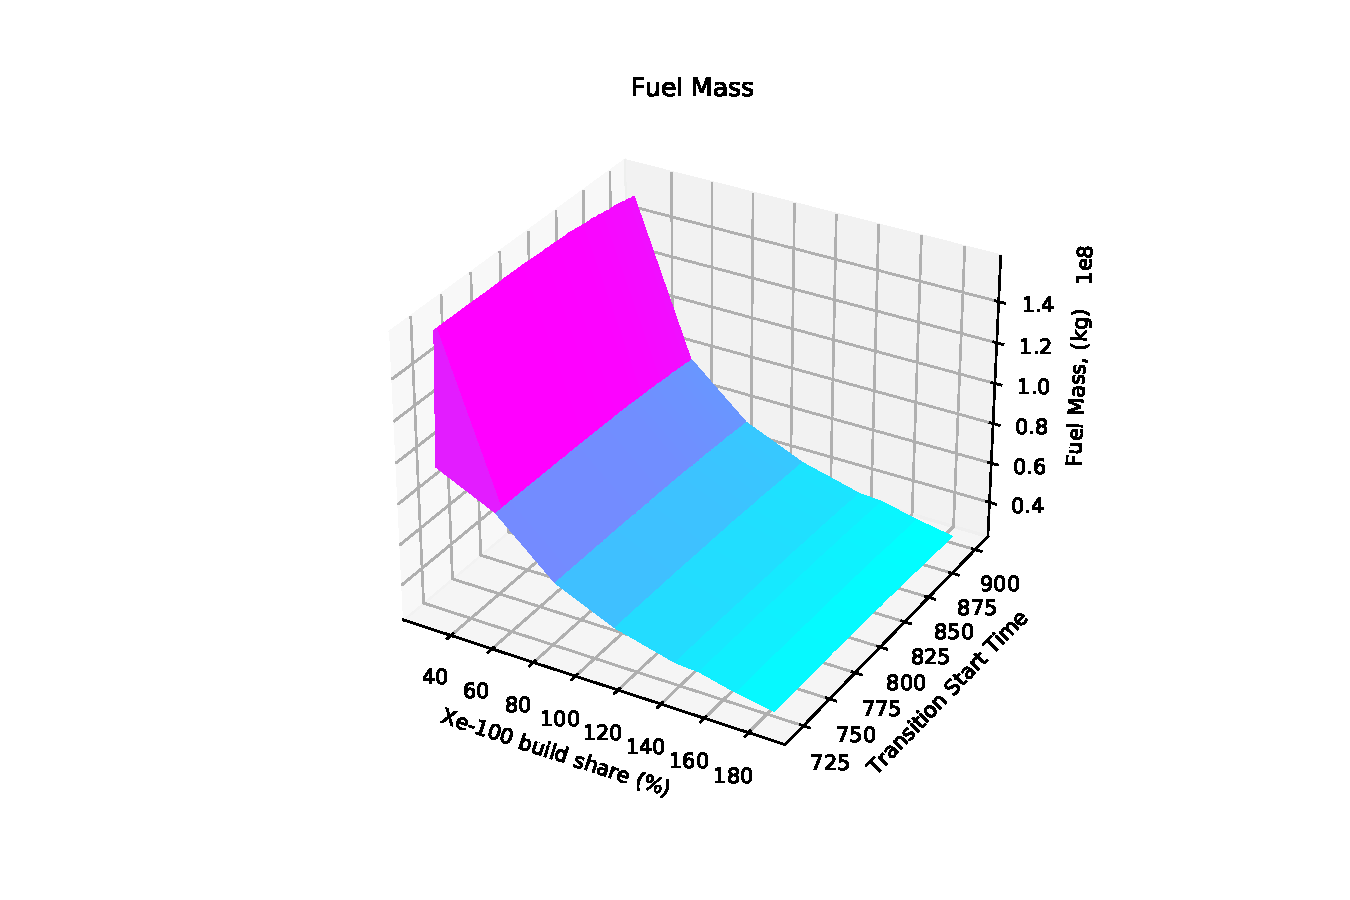
\includegraphics[width=\textwidth, trim=120 0 120 30, clip]{ts_xe100_burnup_enr_u.pdf}
        \caption{Effect on total fuel mass.}
        \label{fig:ts_xe100_bu_enr_u}
    \end{subfigure}
    \hfill
    \begin{subfigure}[h!]{0.48\textwidth}
        \centering
        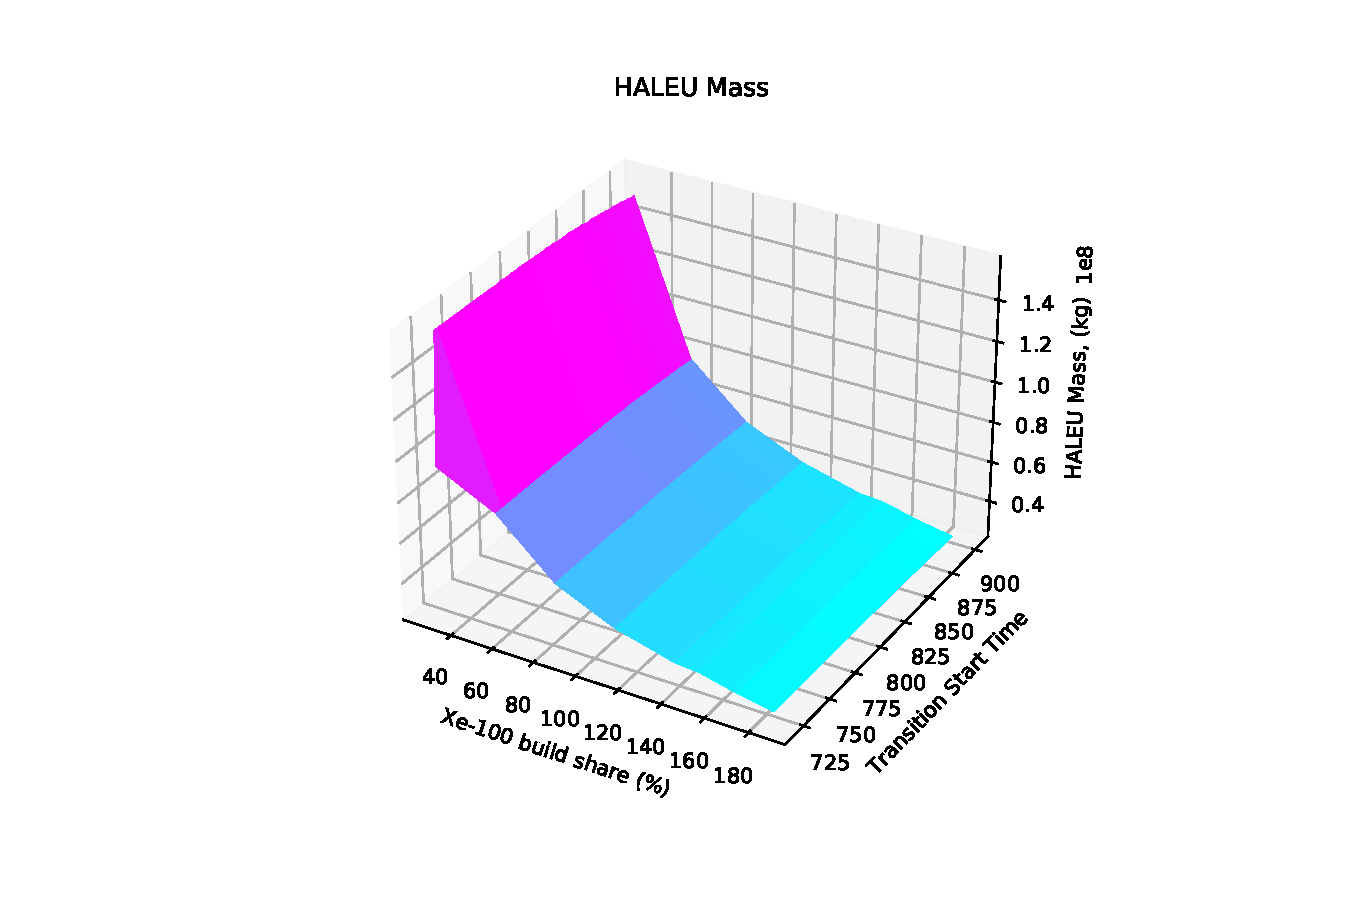
\includegraphics[width=\textwidth, trim=120 0 120 30, clip]{ts_xe100_burnup_haleu.pdf}
        \caption{Effect on HALEU mass.}
        \label{fig:ts_xe100_bu_haleu}
    \end{subfigure}
    
    \begin{subfigure}[h!]{0.48\textwidth}
        \centering
        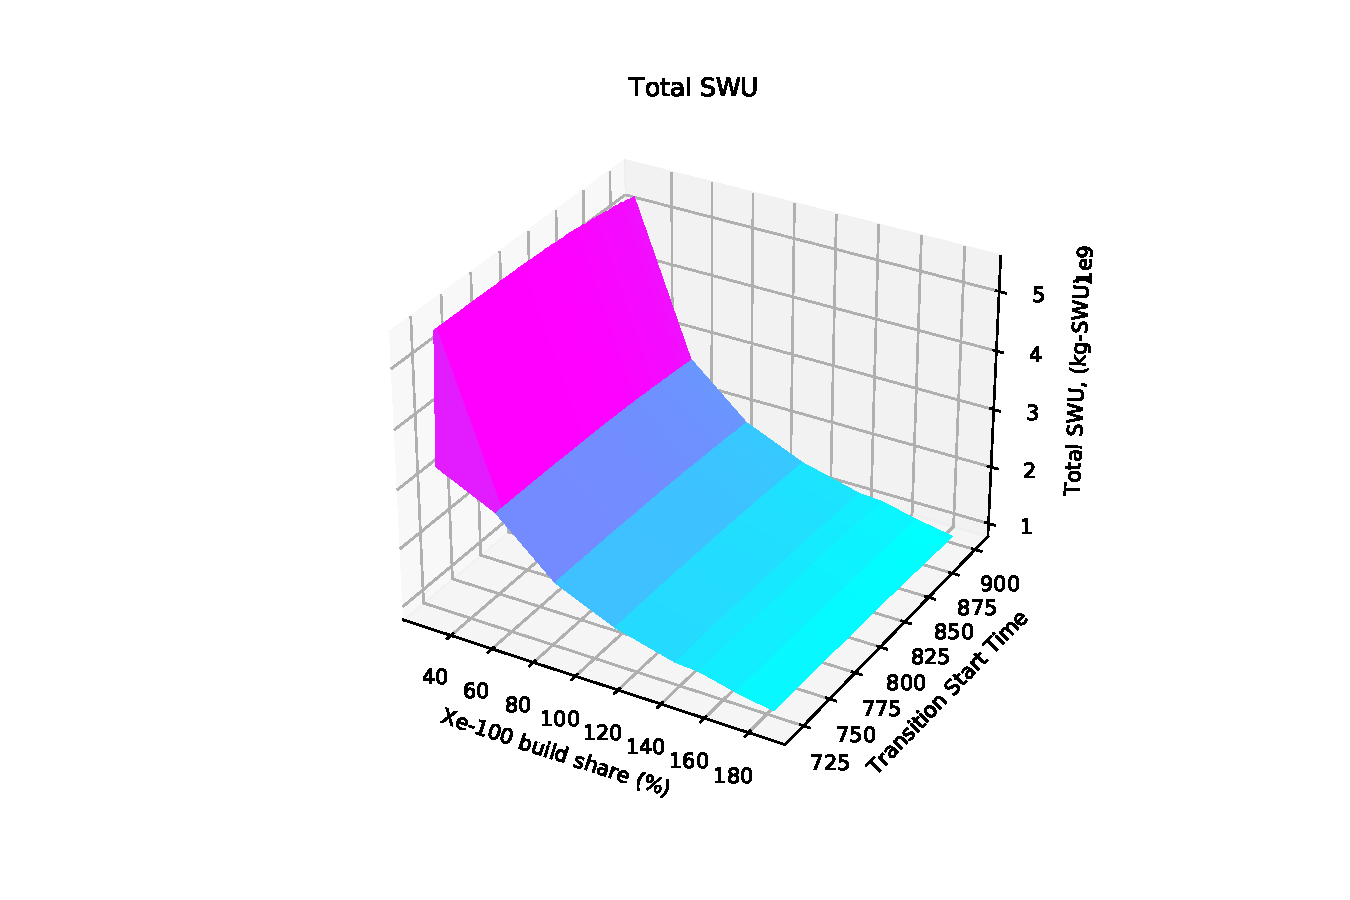
\includegraphics[width=\textwidth, trim=120 0 120 30, clip]{ts_xe100_burnup_swu.pdf}
        \caption{Effect on total SWU capacity.}
        \label{fig:ts_xe100_bu_swu}
    \end{subfigure}
    \hfill
    \begin{subfigure}[h!]{0.48\textwidth}
        \centering
        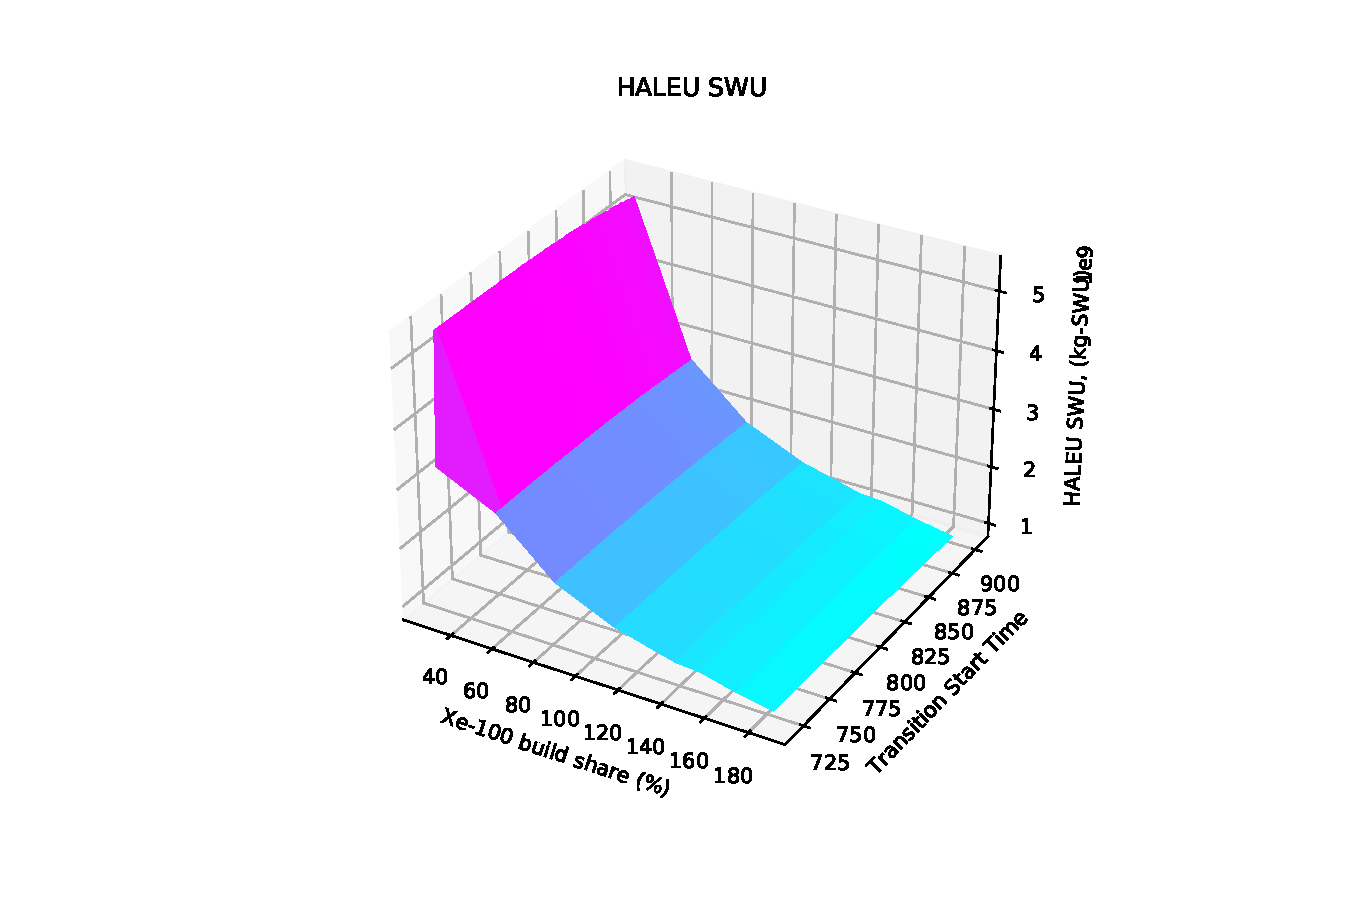
\includegraphics[width=\textwidth, trim=120 0 120 30, clip]{ts_xe100_burnup_haleu_swu.pdf}
        \caption{Effect on HALEU SWU capacity.}
        \label{fig:ts_xe100_bu_haleu_swu}
    \end{subfigure}
    \caption{Change in metrics resulting from variations in the 
    transition start time and Xe-100 burnup.}
\end{figure}

\begin{figure}
    \ContinuedFloat    
    \begin{subfigure}[h!]{0.48\textwidth}
        \centering
        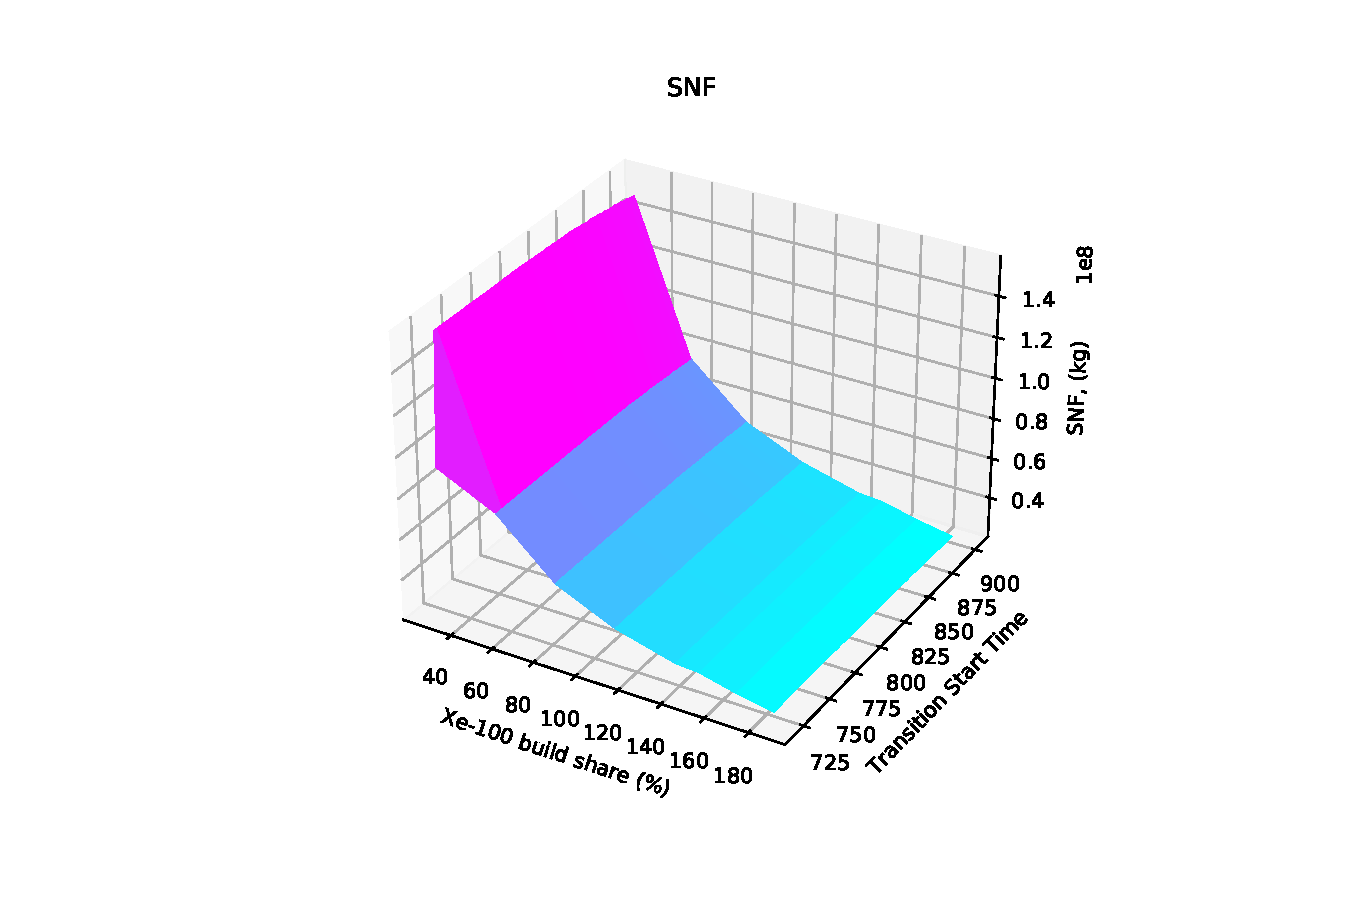
\includegraphics[width=\textwidth, trim=120 0 120 30, clip]{ts_xe100_burnup_waste.pdf}
        \caption{Effect on waste mass discharged.}
        \label{fig:ts_xe100_bu_waste}
    \end{subfigure}
    \hfill
    \begin{subfigure}[h!]{0.48\textwidth}
        \centering
        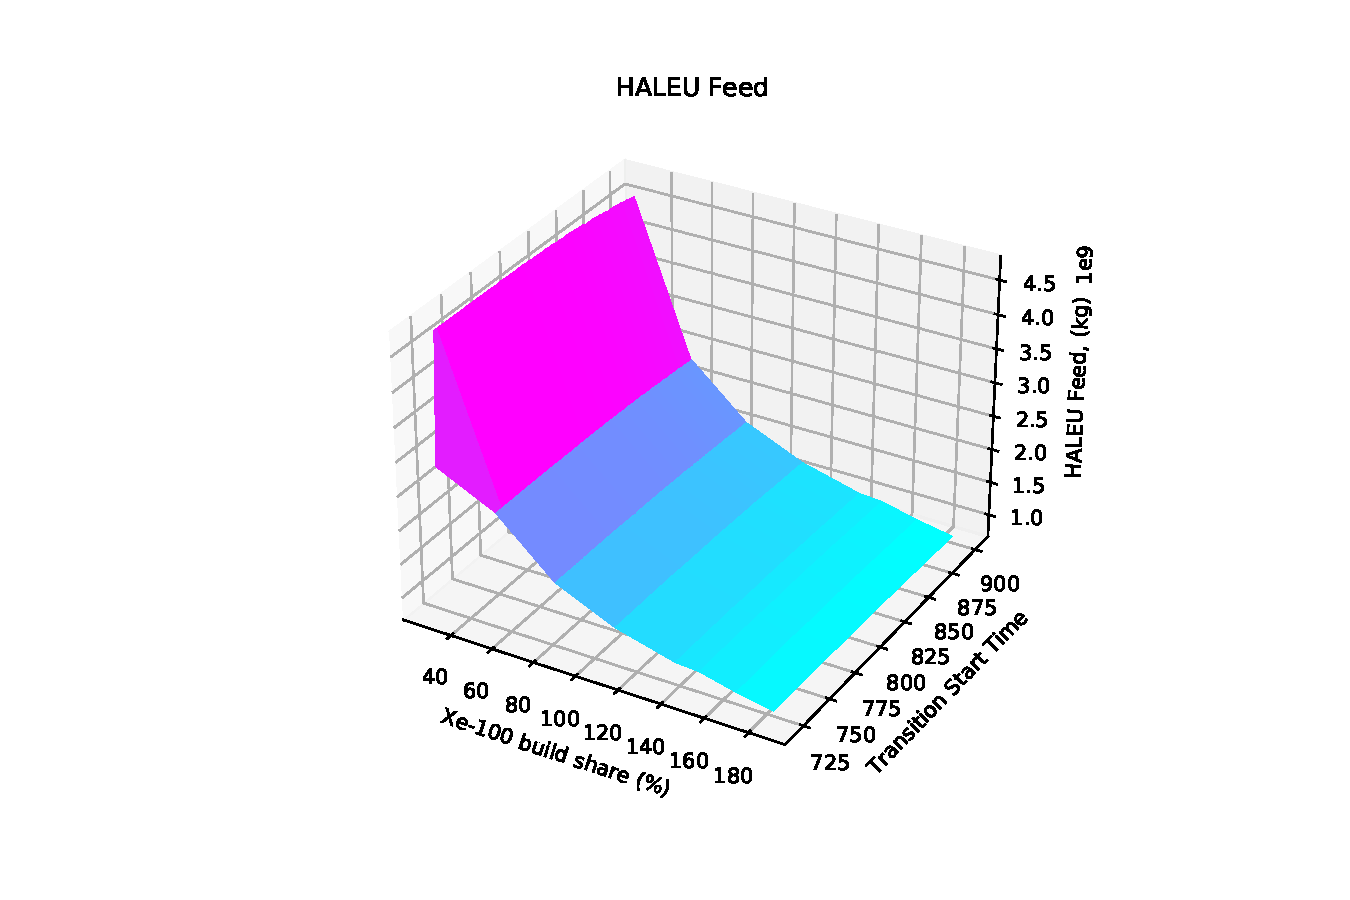
\includegraphics[width=\textwidth, trim=120 0 120 30, clip]{ts_xe100_burnup_feed.pdf}
        \caption{Effect on HALEU feed.}
        \label{fig:ts_xe100_bu_feed}
    \end{subfigure}
    \caption{(cont.) Change in metrics resulting from variations in the 
    transition start time and Xe-100 burnup.}
    \label{fig:ts_xe100_bu}
\end{figure}

Figure \ref{fig:ts_mmr_bu} shows the effects of varying the transition 
start time and the \gls{MMR} discharge burnup on all six metrics. All 
of the metrics exhibit the same trends as the parameters vary: the 
metrics decrease as the transition start time is later and as the 
\gls{MMR} burnup increases. The two parameters have impacts on similar 
magnitudes, which is in contrast to the impact from the Xe-100 burnup. The 
\gls{MMR} burnup has a smaller impact on the metrics because \glspl{MMR} 
make up a smaller fraction of the advanced reactor fleet than Xe-100s. 

\begin{figure}
    \begin{subfigure}[h!]{0.48\textwidth}
        \centering
        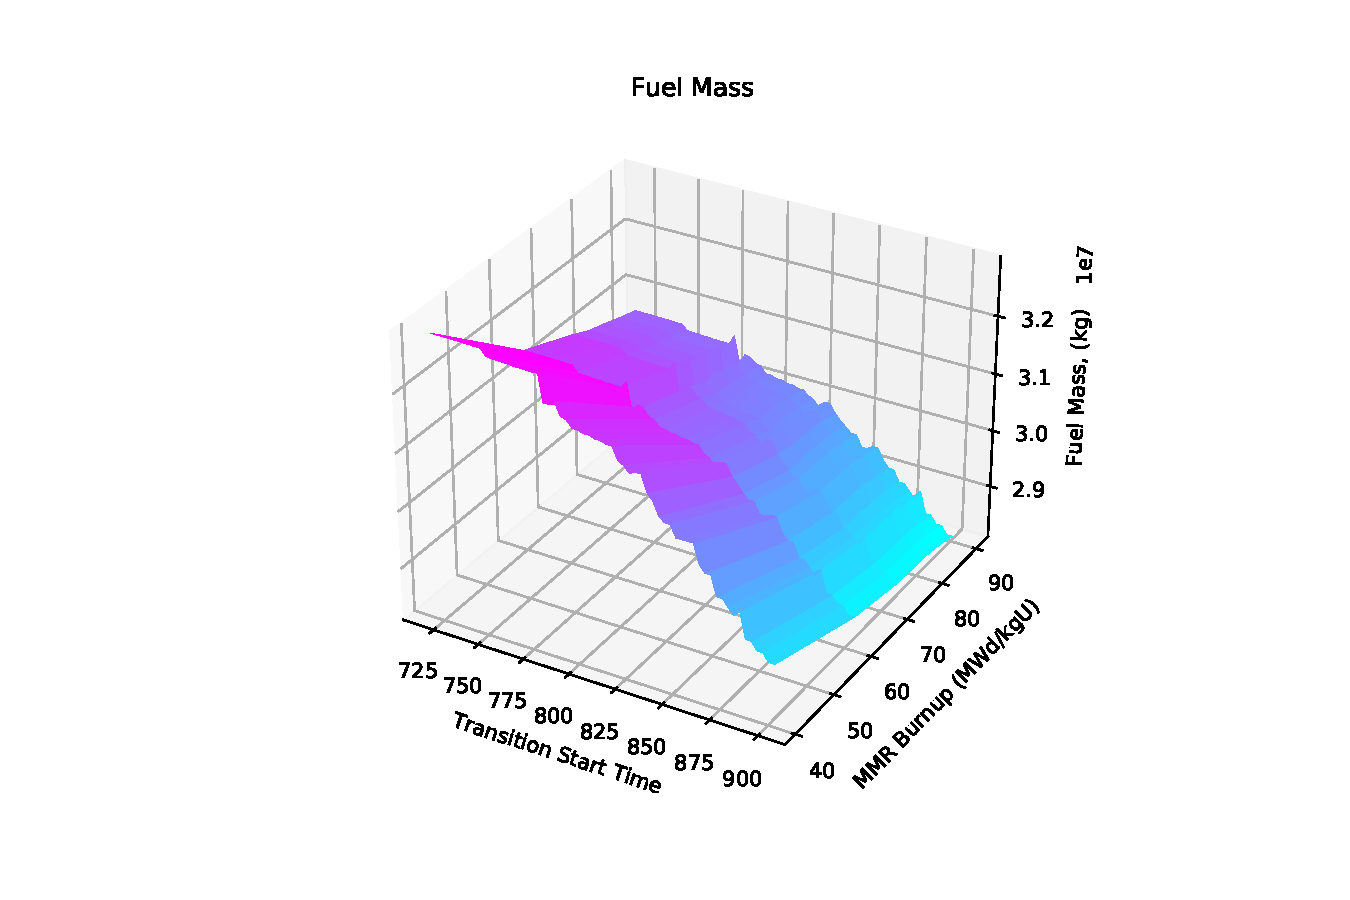
\includegraphics[width=\textwidth, trim=120 0 120 30, clip]{ts_mmr_burnup_enr_u.pdf}
        \caption{Effect on total fuel mass.}
        \label{fig:ts_mmr_bu_enr_u}
    \end{subfigure}
    \hfill
    \begin{subfigure}[h!]{0.48\textwidth}
        \centering
        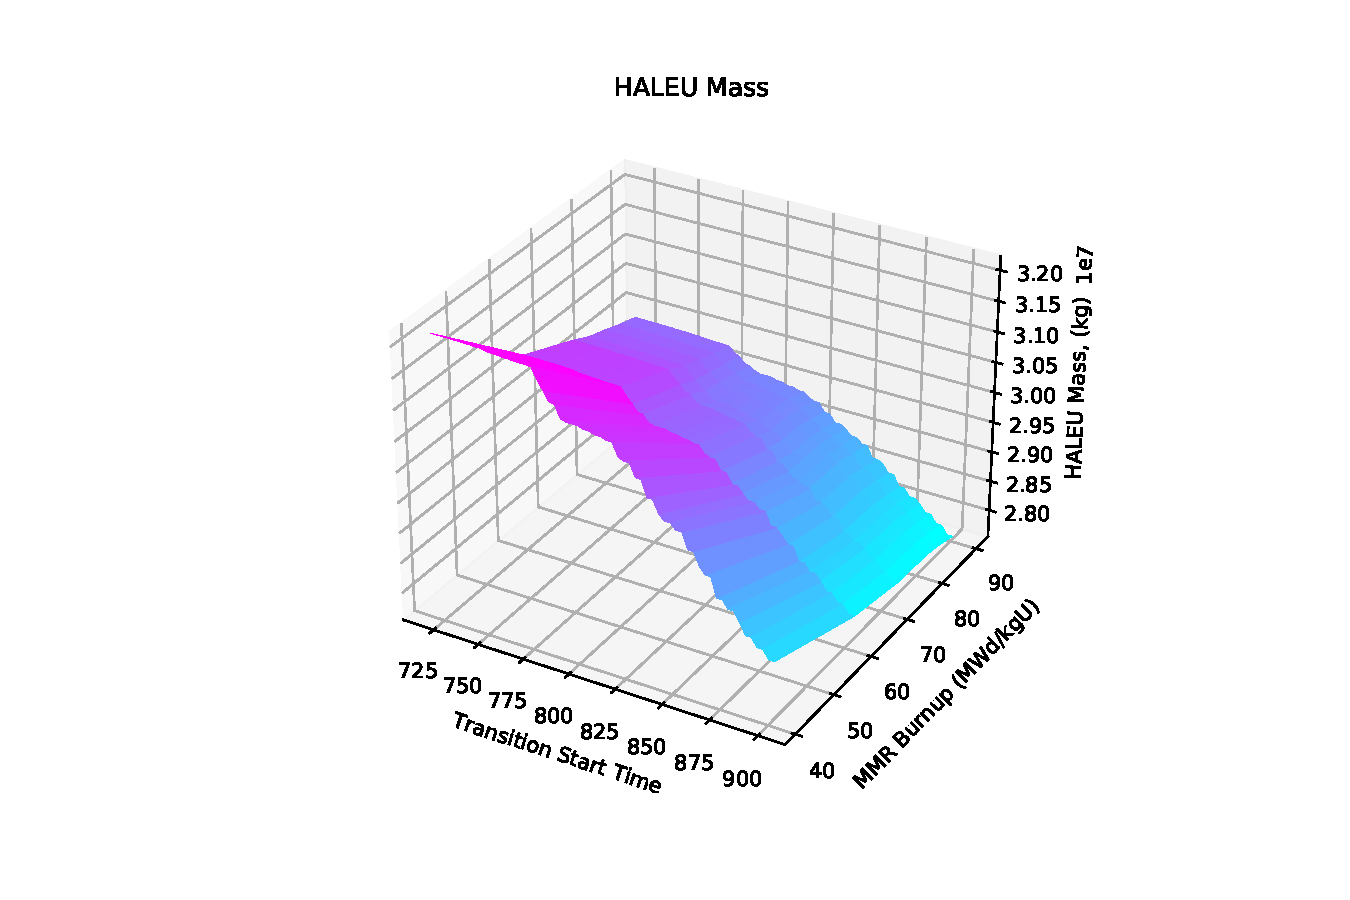
\includegraphics[width=\textwidth, trim=120 0 120 30, clip]{ts_mmr_burnup_haleu.pdf}
        \caption{Effect on HALEU mass.}
        \label{fig:ts_mmr_bu_haleu}
    \end{subfigure}
    \caption{Change in metrics resulting from variations in the 
    transition start time and MMR burnup.}
\end{figure}

\begin{figure}
    \ContinuedFloat    
    \begin{subfigure}[h!]{0.48\textwidth}
        \centering
        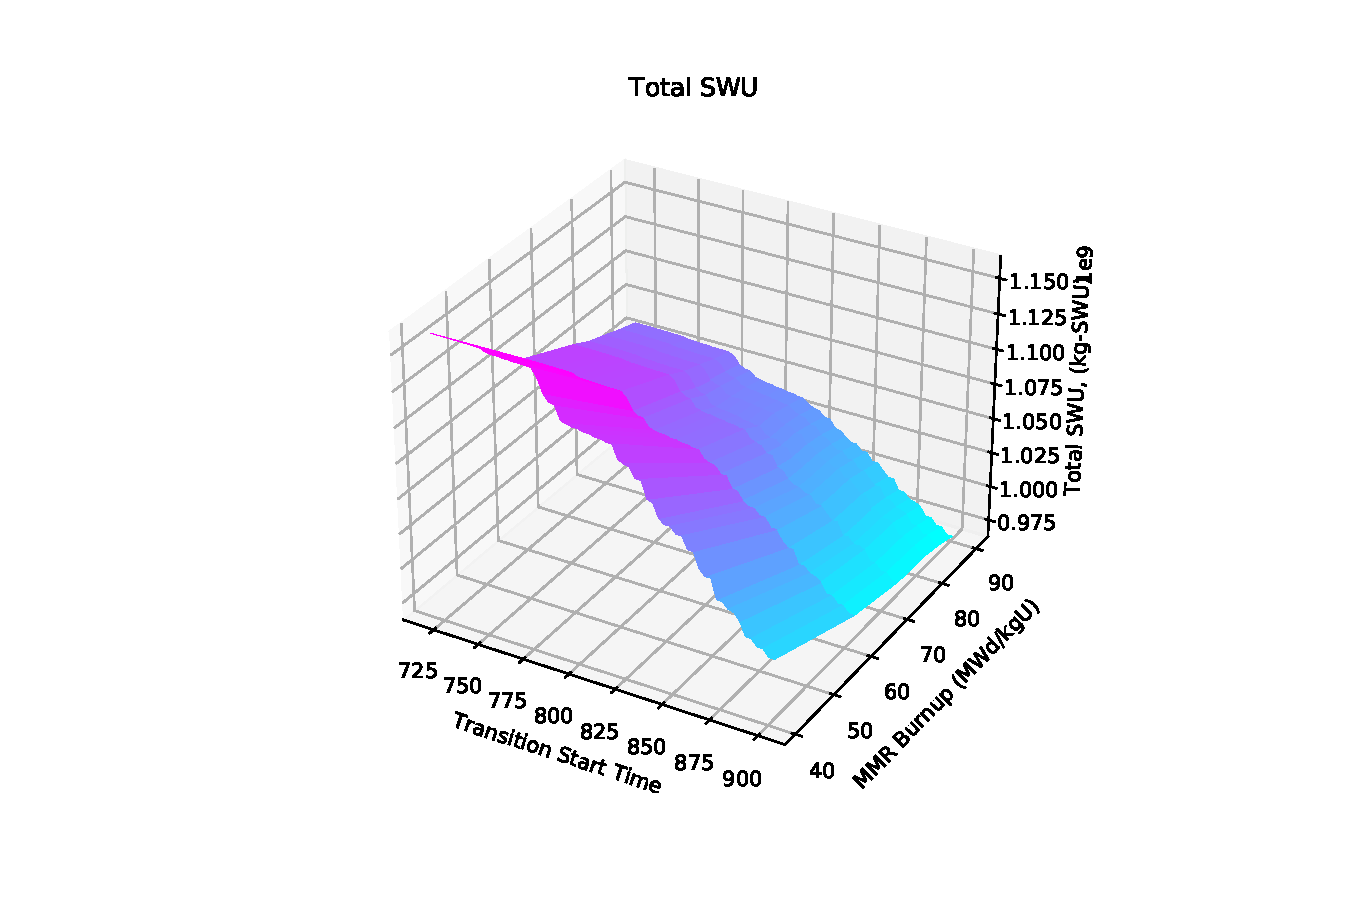
\includegraphics[width=\textwidth, trim=120 0 120 30, clip]{ts_mmr_burnup_swu.pdf}
        \caption{Effect on total SWU capacity.}
        \label{fig:ts_mmr_bu_swu}
    \end{subfigure}
    \hfill
    \begin{subfigure}[h!]{0.48\textwidth}
        \centering
        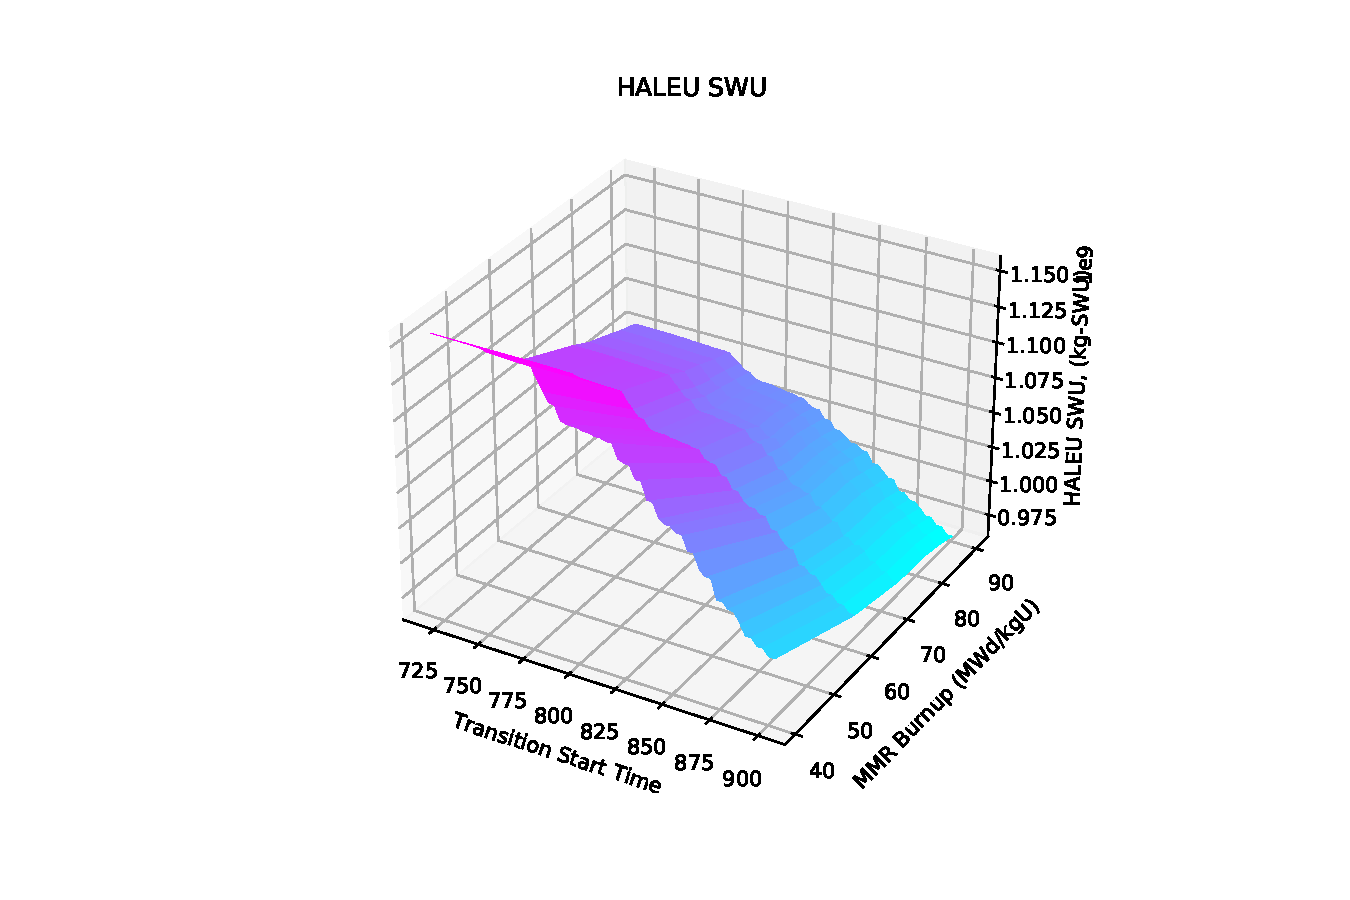
\includegraphics[width=\textwidth, trim=120 0 120 30, clip]{ts_mmr_burnup_haleu_swu.pdf}
        \caption{Effect on HALEU SWU capacity.}
        \label{fig:ts_mmr_bu_haleu_swu}
    \end{subfigure}
    
    \begin{subfigure}[h!]{0.48\textwidth}
        \centering
        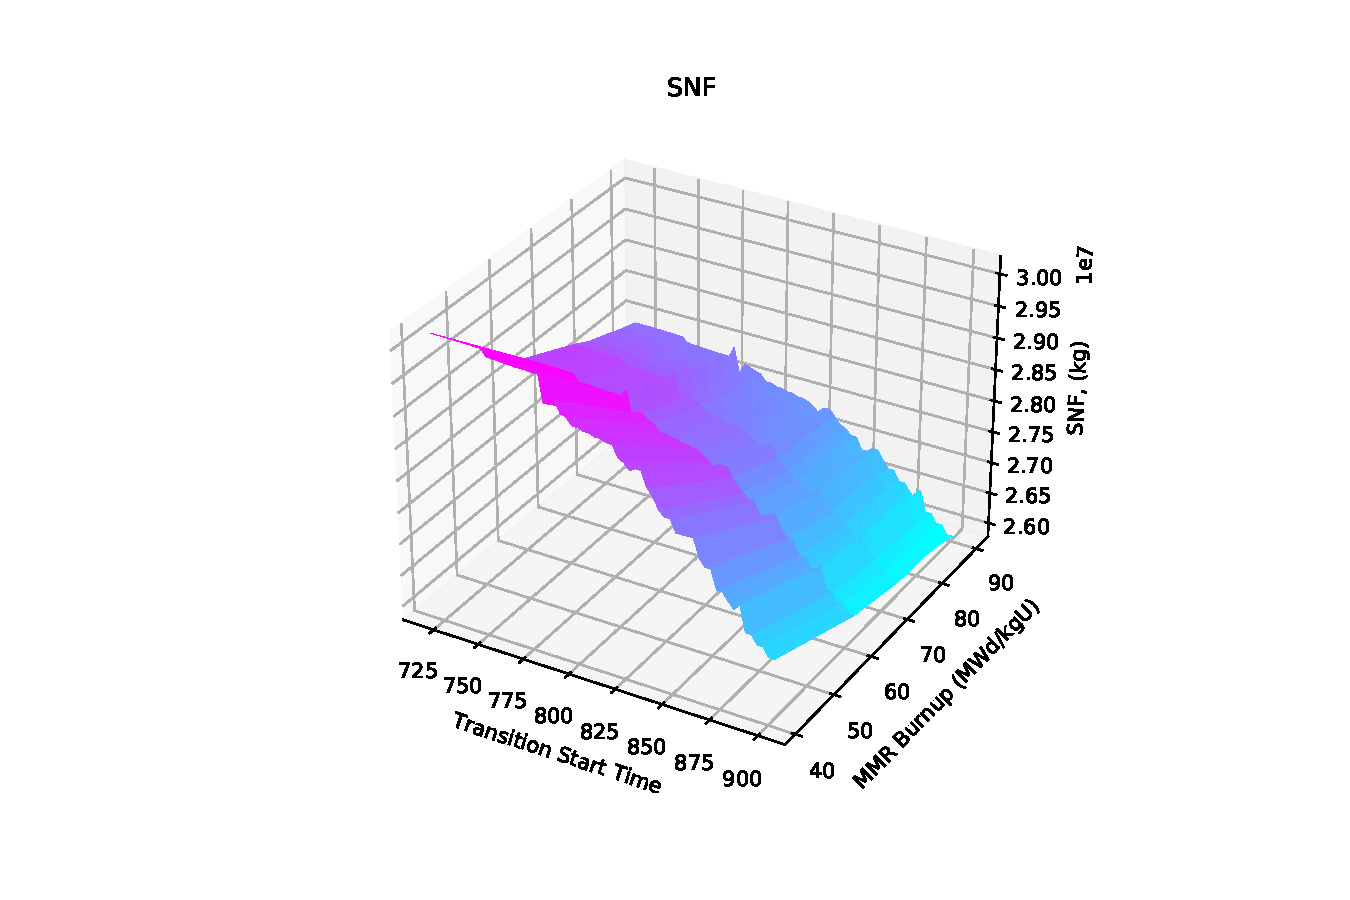
\includegraphics[width=\textwidth, trim=120 0 120 30, clip]{ts_mmr_burnup_waste.pdf}
        \caption{Effect on waste mass discharged.}
        \label{fig:ts_mmr_bu_waste}
    \end{subfigure}
    \hfill
    \begin{subfigure}[h!]{0.48\textwidth}
        \centering
        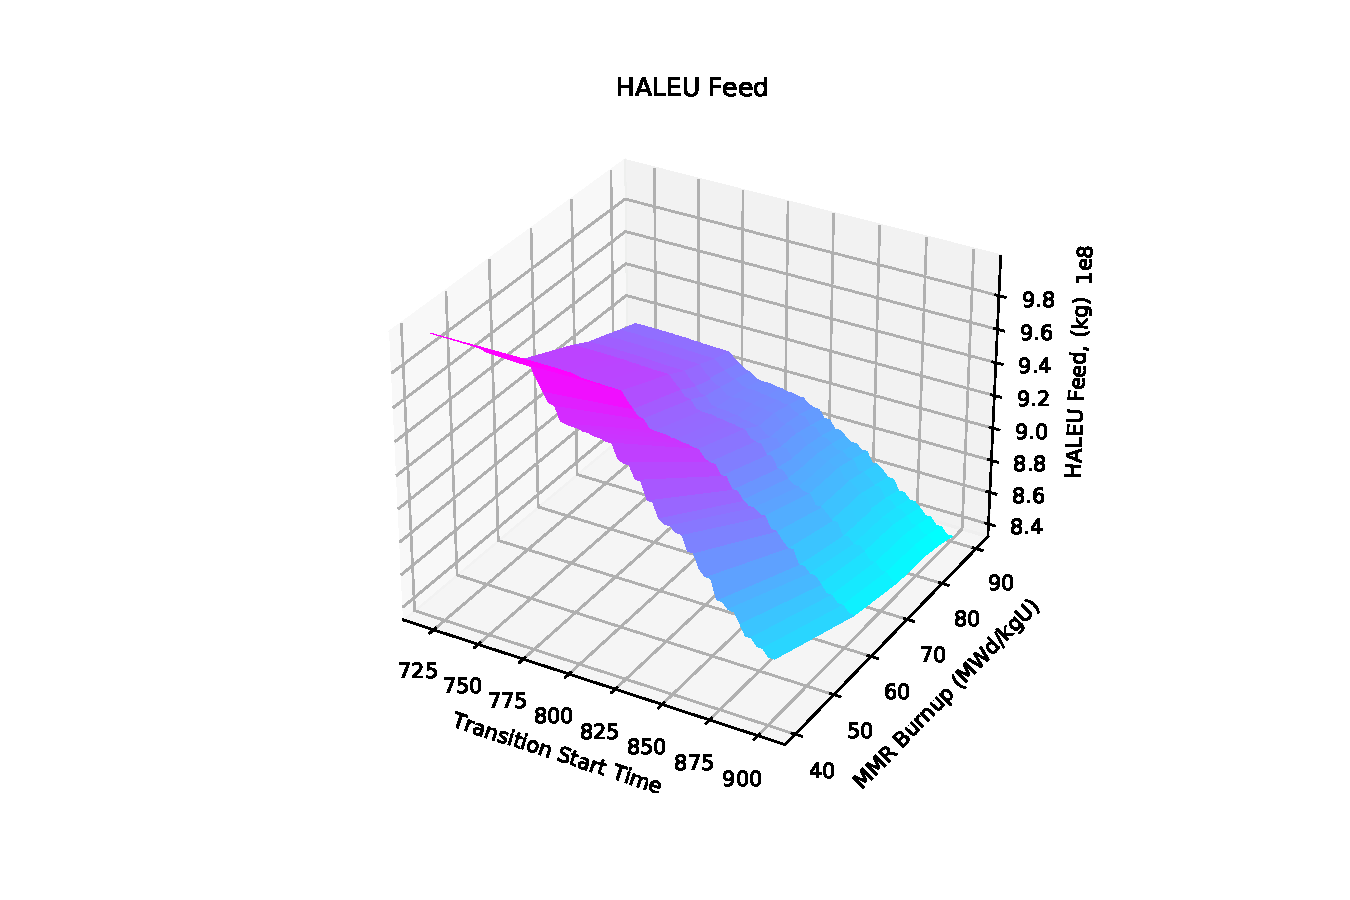
\includegraphics[width=\textwidth, trim=120 0 120 30, clip]{ts_mmr_burnup_feed.pdf}
        \caption{Effect on HALEU feed.}
        \label{fig:ts_mmr_bu_feed}
    \end{subfigure}
    \caption{(cont.) Change in metrics resulting from variations in the 
    transition start time and MMR burnup.}
    \label{fig:ts_mmr_bu}
\end{figure}

Figure \ref{fig:lwr_xe100_share} shows the effects of varying the 
percent of \glspl{LWR} operating for 80 years and the Xe-100 
build share on all six metrics. The trends observed in the \gls{OAT} 
can also be observed here, such as how increasing the Xe-100 share 
increases the \gls{HALEU} mass required but increasing the 
percent of \glspl{LWR} decreases this metric. However, these results 
show that there is a combined effect from varying these parameters 
together that is not captured in the \gls{OAT} analysis. For 
example, the \gls{HALEU} mass (Figure \ref{fig:lwr_xe100_share_haleu}) 
decreases by a greater fraction 
as the percent of \glspl{LWR} and Xe-100 build shares increase than 
when only the percent of \glspl{LWR} extended increases. This combined 
effect is a result of more of the advanced reactor fleet being fueled 
by \gls{HALEU}-fueled reactors. However, these results also show that 
the despite this combined effect, not deploying Xe-100s will still
result in a minimum in the \gls{HALEU} mass required. This trend is also 
observed in the other \gls{HALEU}-related metrics (Figures \ref{fig:lwr_xe100_share_haleu_swu},
and \ref{fig:lwr_xe100_share_feed}). 

The total fuel (Figure \ref{fig:lwr_xe100_share_enr_u}) and used fuel 
mass (Figure \ref{fig:lwr_xe100_share_waste}) both exhibit a different trend 
than the \gls{HALEU}-related metrics. These two parameters have a similar 
effect on these metrics: as the parameter values increase, the metric value 
decreases. Therefore, by increasing both of these parameters, there is a 
larger effect on the total and used fuel masses than varying each on 
separately. 

\begin{figure}
    \begin{subfigure}[h!]{0.48\textwidth}
        \centering
        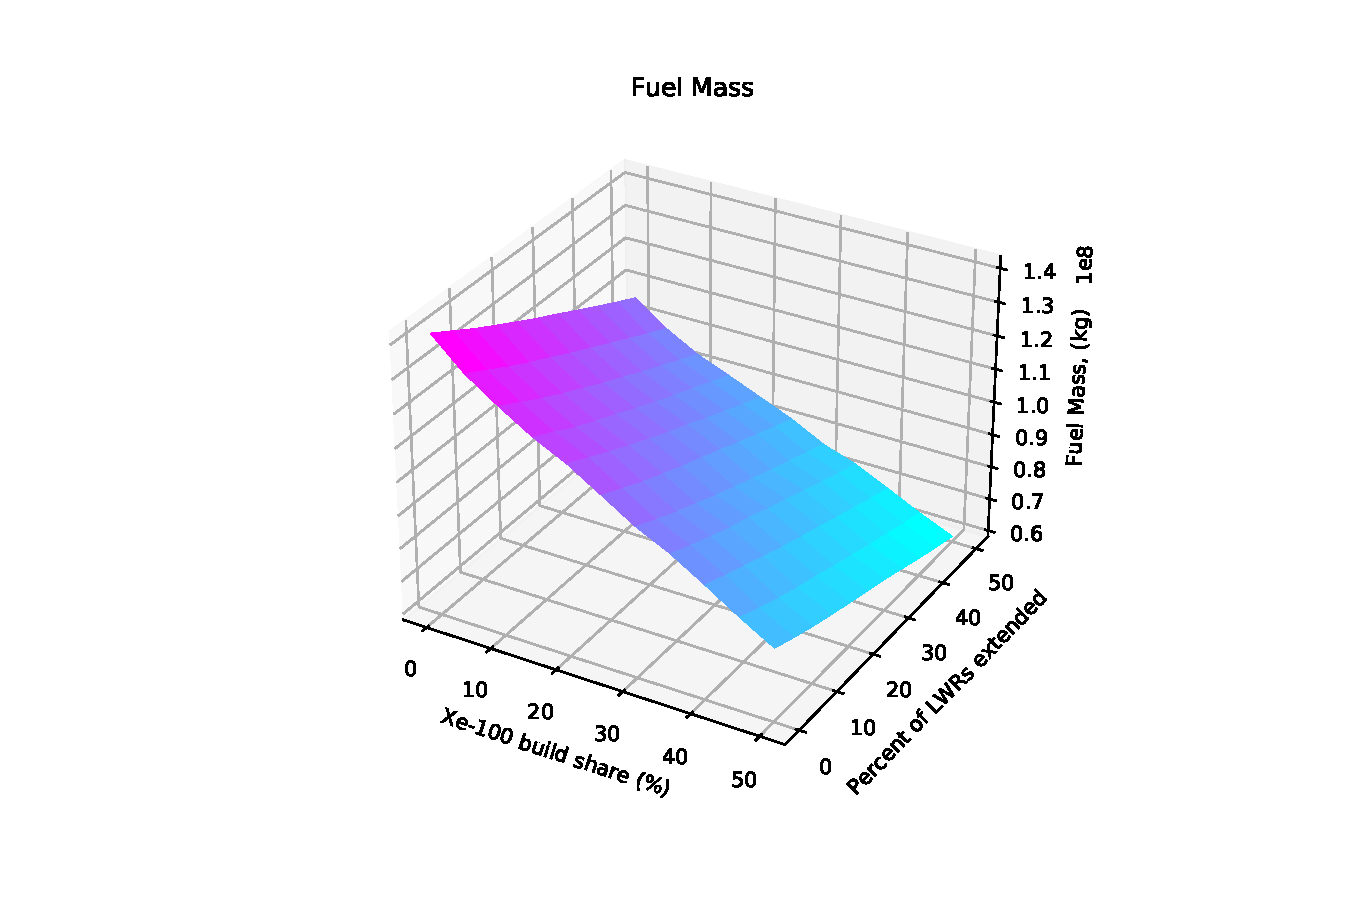
\includegraphics[width=\textwidth, trim=120 0 120 30, clip]{lwr_xe100_share_enr_u.pdf}
        \caption{Effect on total fuel mass.}
        \label{fig:lwr_xe100_share_enr_u}
    \end{subfigure}
    \hfill
    \begin{subfigure}[h!]{0.48\textwidth}
        \centering
        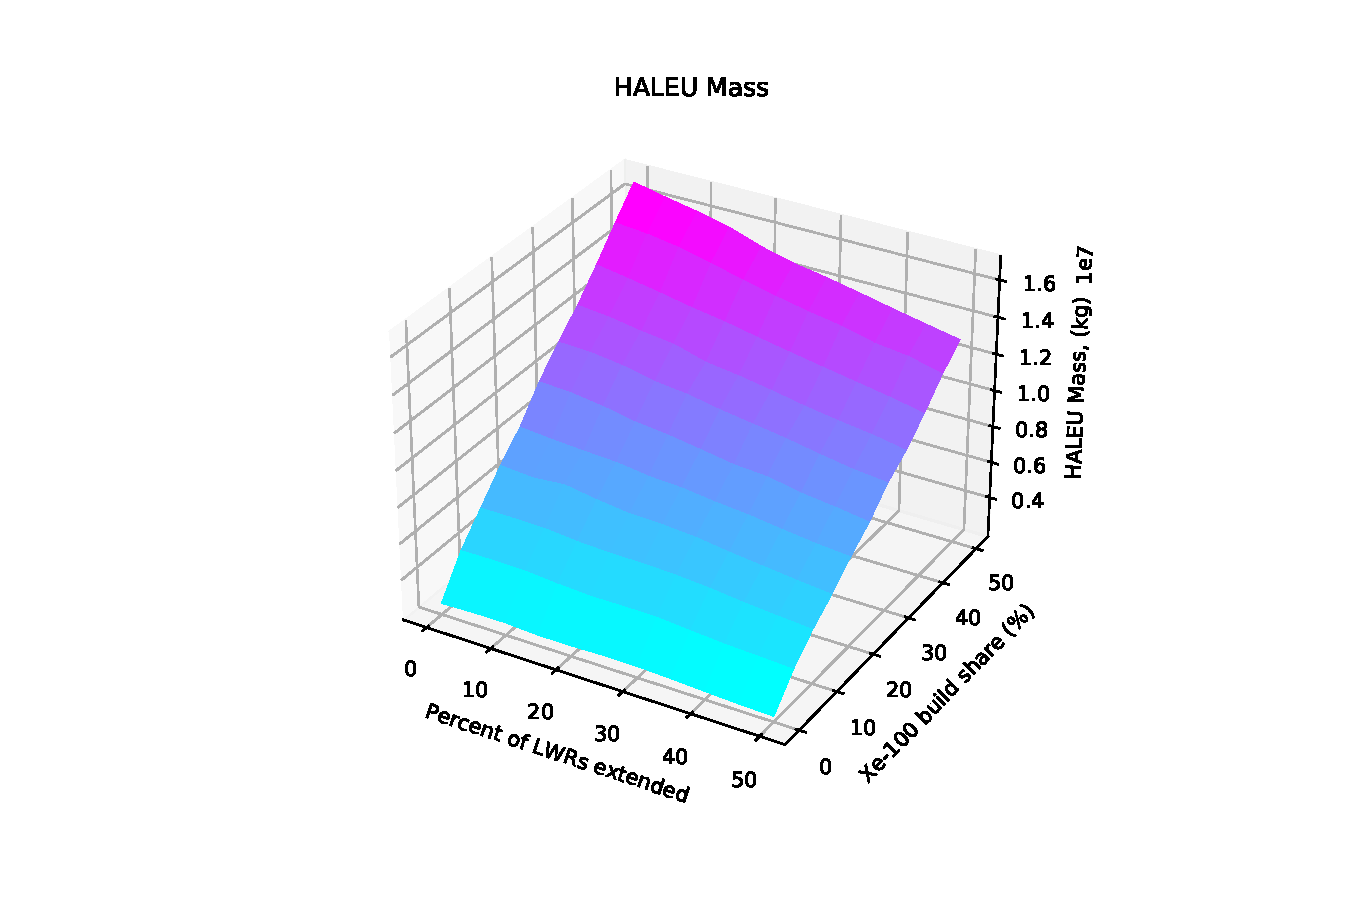
\includegraphics[width=\textwidth, trim=120 0 120 30, clip]{lwr_xe100_share_haleu.pdf}
        \caption{Effect on HALEU mass.}
        \label{fig:lwr_xe100_share_haleu}
    \end{subfigure}  
    \begin{subfigure}[h!]{0.48\textwidth}
        \centering
        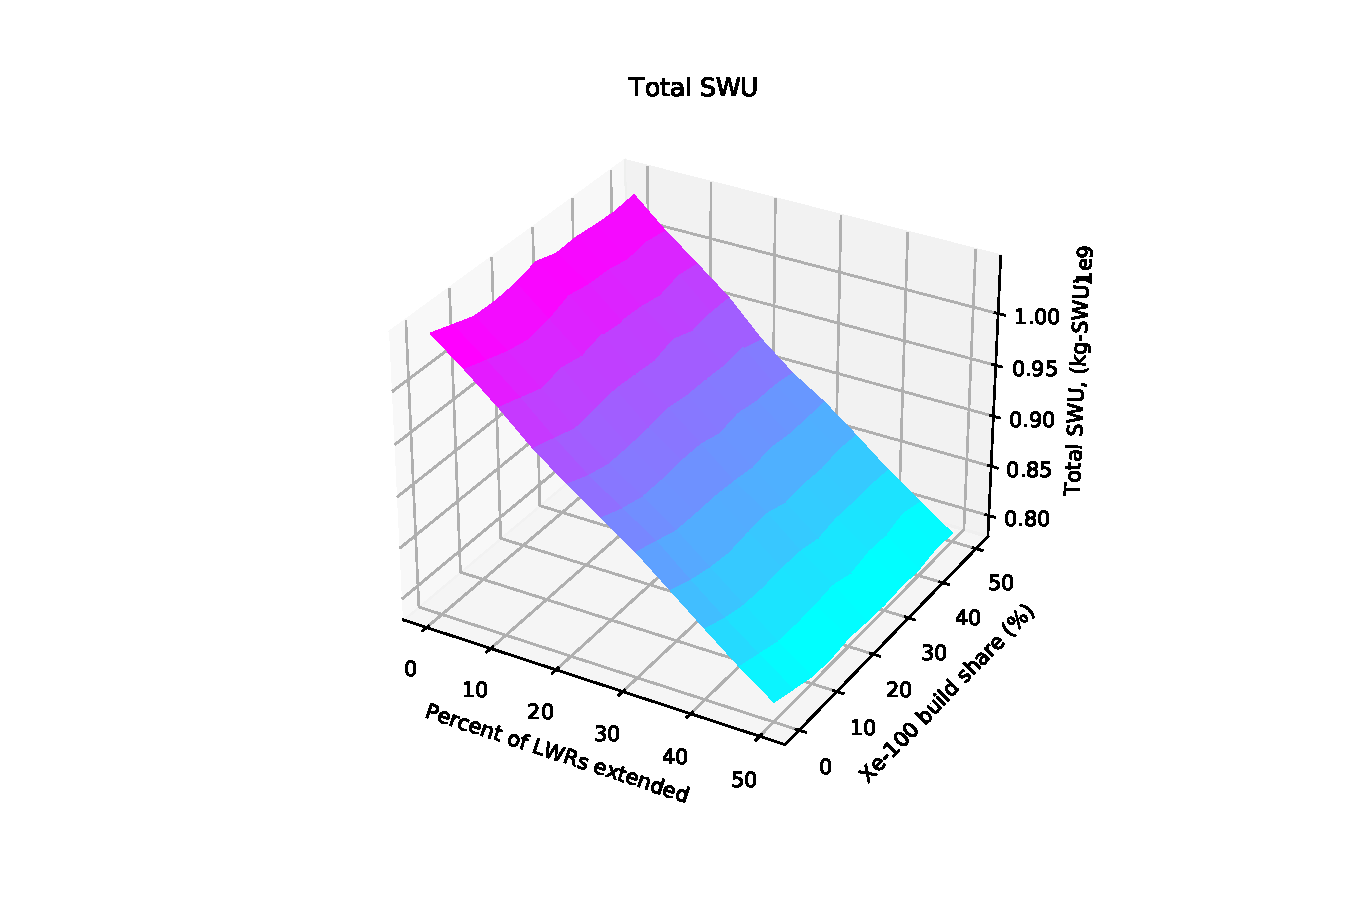
\includegraphics[width=\textwidth, trim=120 0 120 30, clip]{lwr_xe100_share_swu.pdf}
        \caption{Effect on total SWU capacity.}
        \label{fig:lwr_xe100_share_swu}
    \end{subfigure}
    \hfill
    \begin{subfigure}[h!]{0.48\textwidth}
        \centering
        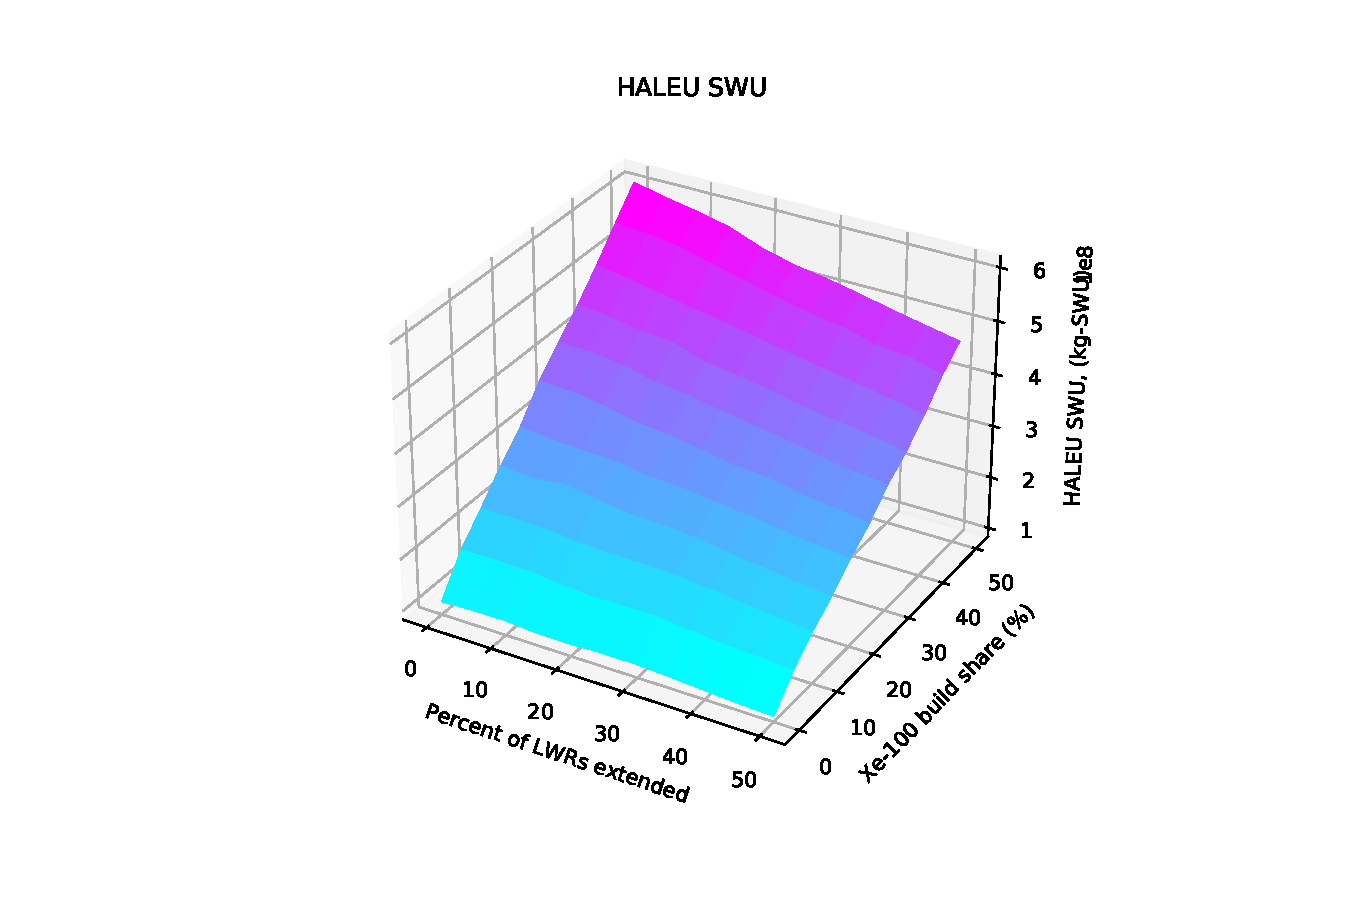
\includegraphics[width=\textwidth, trim=120 0 120 30, clip]{lwr_xe100_share_haleu_swu.pdf}
        \caption{Effect on HALEU SWU capacity.}
        \label{fig:lwr_xe100_share_haleu_swu}
    \end{subfigure}
    \caption{Change in metrics resulting from variations in the 
    LWR lifetimes and Xe-100 build share.}
\end{figure}

\begin{figure}
    \ContinuedFloat    
    \begin{subfigure}[h!]{0.48\textwidth}
        \centering
        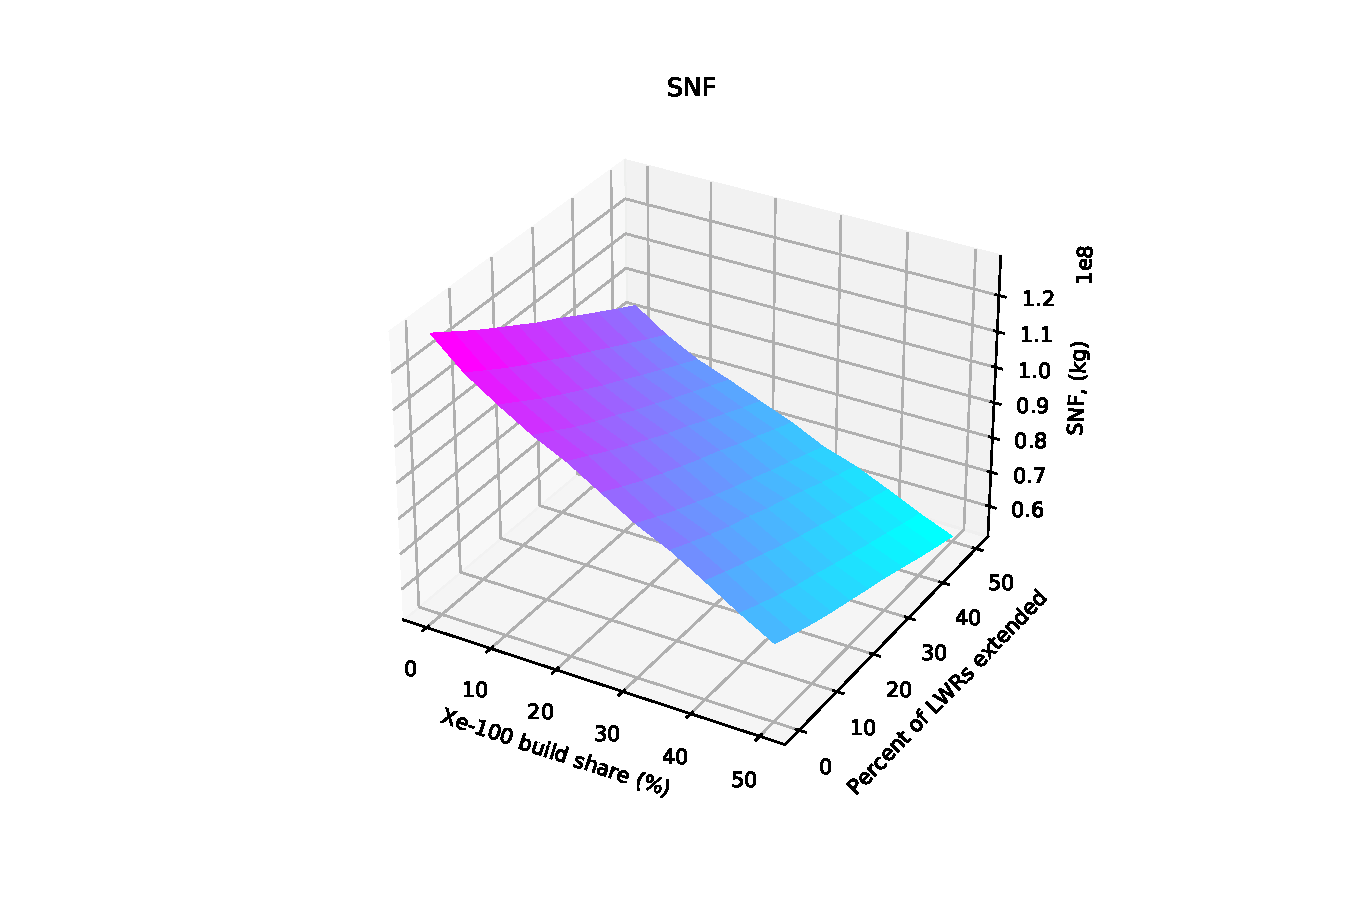
\includegraphics[width=\textwidth, trim=120 0 120 30, clip]{lwr_xe100_share_waste.pdf}
        \caption{Effect on waste mass discharged.}
        \label{fig:lwr_xe100_share_waste}
    \end{subfigure}
    \hfill
    \begin{subfigure}[h!]{0.48\textwidth}
        \centering
        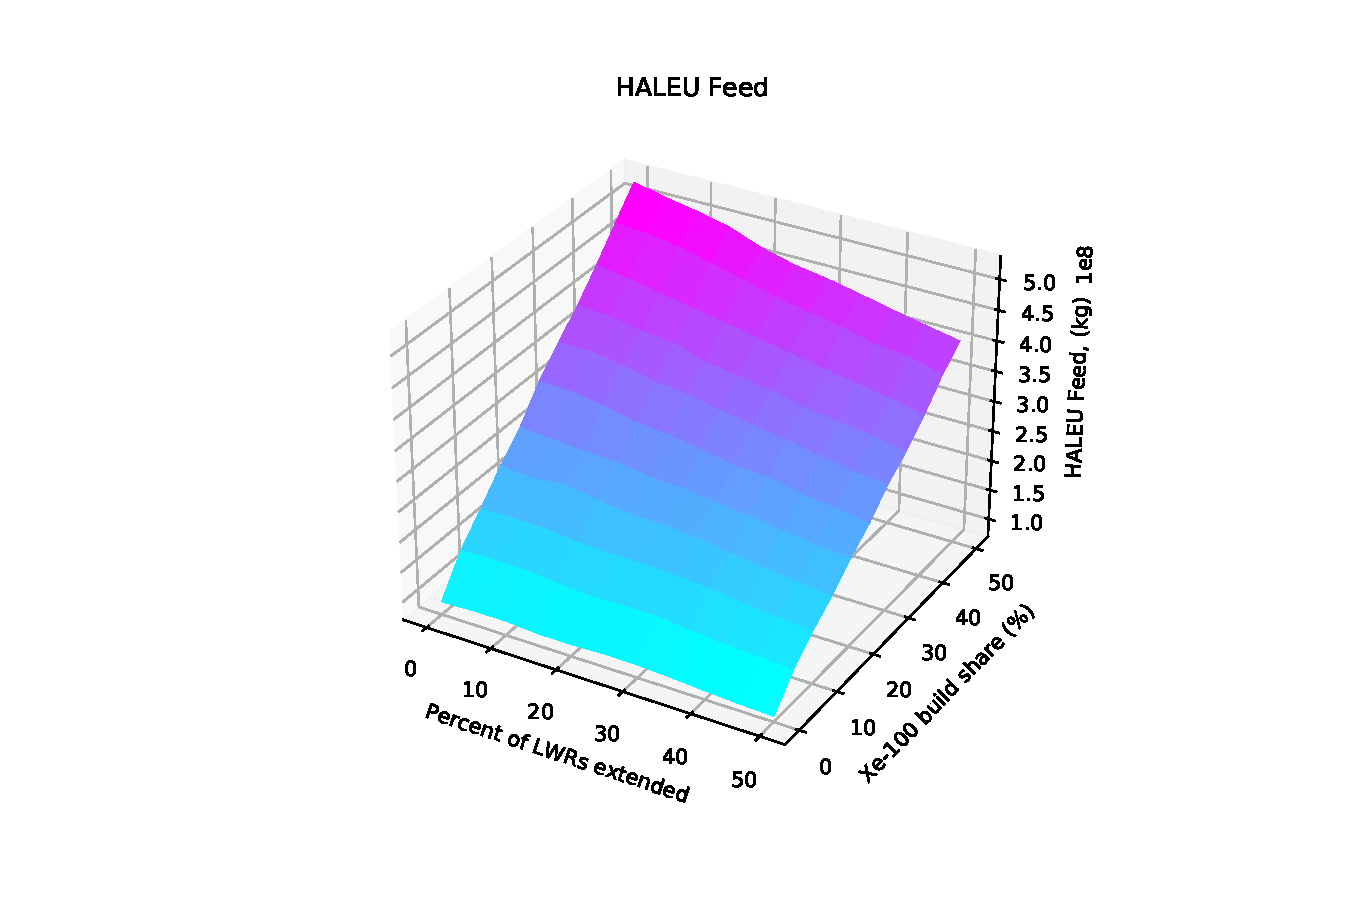
\includegraphics[width=\textwidth, trim=120 0 120 30, clip]{lwr_xe100_share_feed.pdf}
        \caption{Effect on HALEU feed.}
        \label{fig:lwr_xe100_share_feed}
    \end{subfigure}
    \caption{(cont.) Change in metrics resulting from variations in the 
    LWR lifetimes and Xe-100 build share.}
    \label{fig:lwr_xe100_share}
\end{figure}

Figure \ref{fig:lwr_mmr_share} shows the effects of varying the 
percent of \glspl{LWR} operating for 80 years and the \gls{MMR} 
build share on all of the metrics. The metrics have the same trends 
as the parameters are varied: they increase as the \gls{MMR} build 
share increases and as the percent of \glspl{LWR} extended 
decreases. Therefore, all six metrics reach a minimum with 50\% of 
the \glspl{LWR} operating for 80 years and a 0\% \gls{MMR} build 
share. 

\begin{figure}
    \begin{subfigure}[h!]{0.48\textwidth}
        \centering
        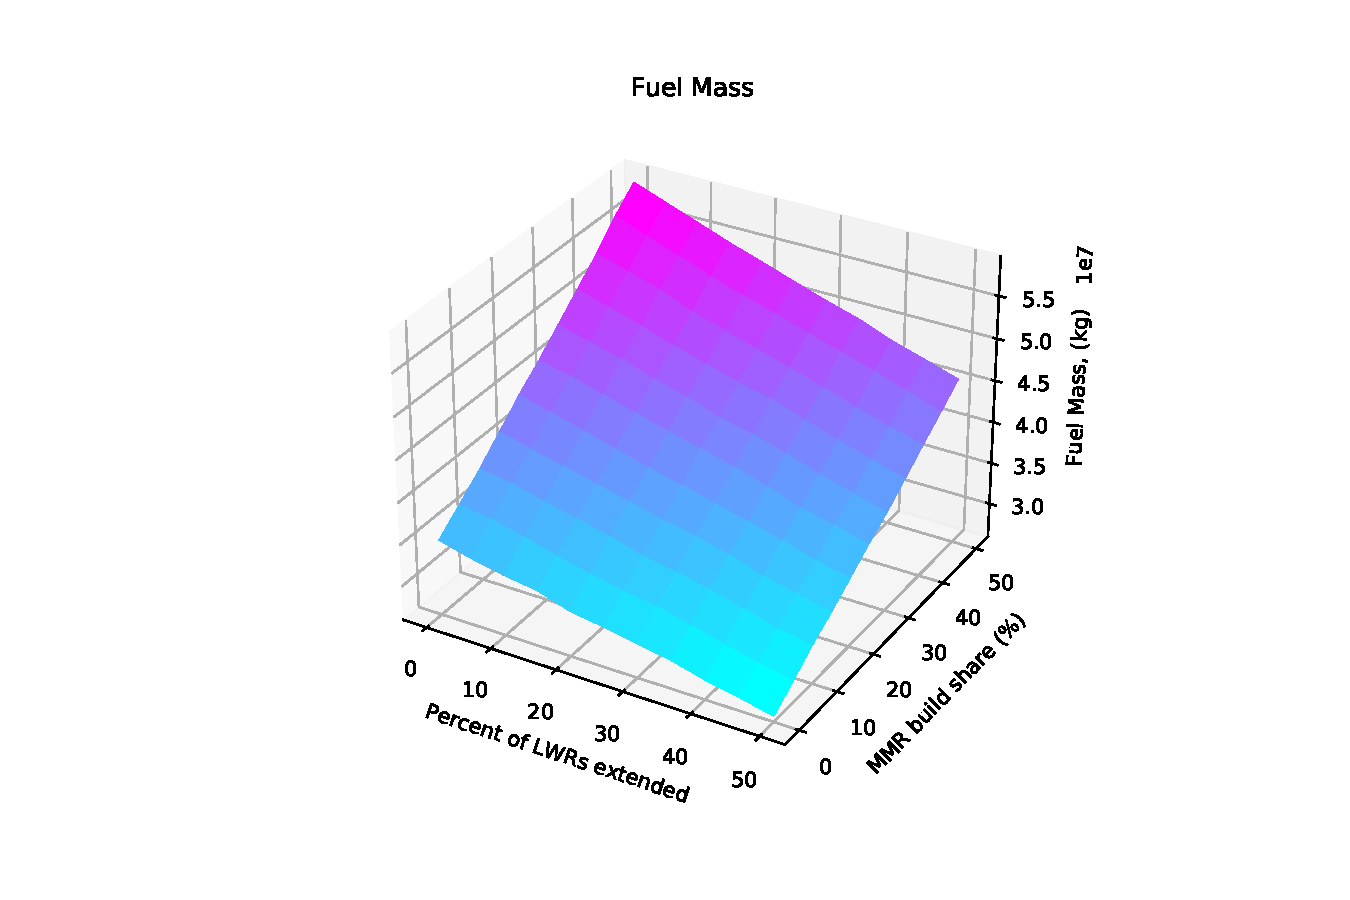
\includegraphics[width=\textwidth, trim=120 0 120 30, clip]{lwr_mmr_share_enr_u.pdf}
        \caption{Effect on total fuel mass.}
        \label{fig:lwr_mmr_share_enr_u}
    \end{subfigure}
    \hfill
    \begin{subfigure}[h!]{0.48\textwidth}
        \centering
        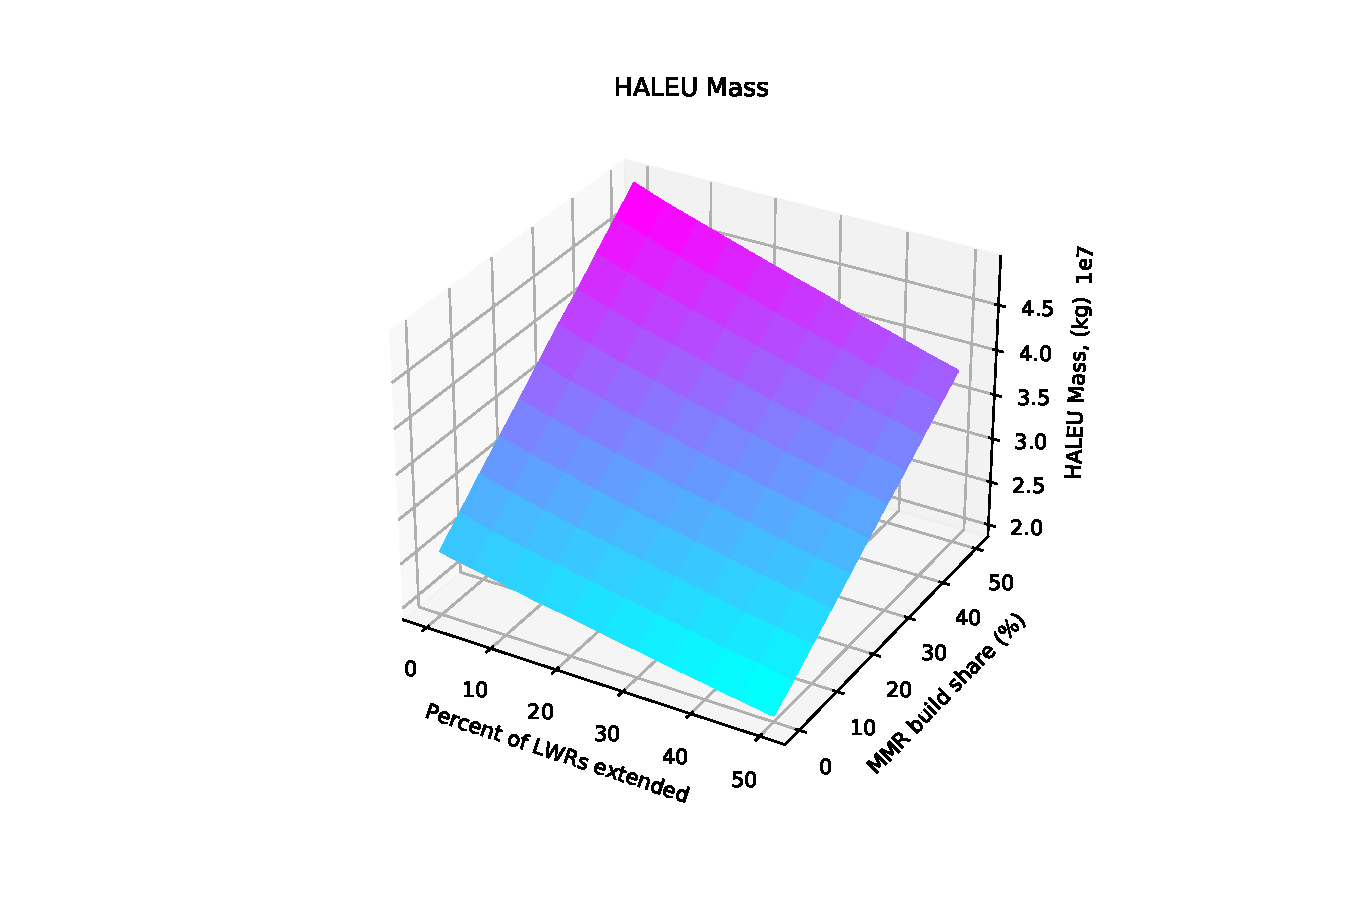
\includegraphics[width=\textwidth, trim=120 0 120 30, clip]{lwr_mmr_share_haleu.pdf}
        \caption{Effect on HALEU mass.}
        \label{fig:lwr_mmr_share_haleu}
    \end{subfigure}
    \caption{Change in metrics resulting from variations in the 
    LWR lifetimes and MMR build share.}
\end{figure}

\begin{figure}
    \ContinuedFloat    
    \begin{subfigure}[h!]{0.48\textwidth}
        \centering
        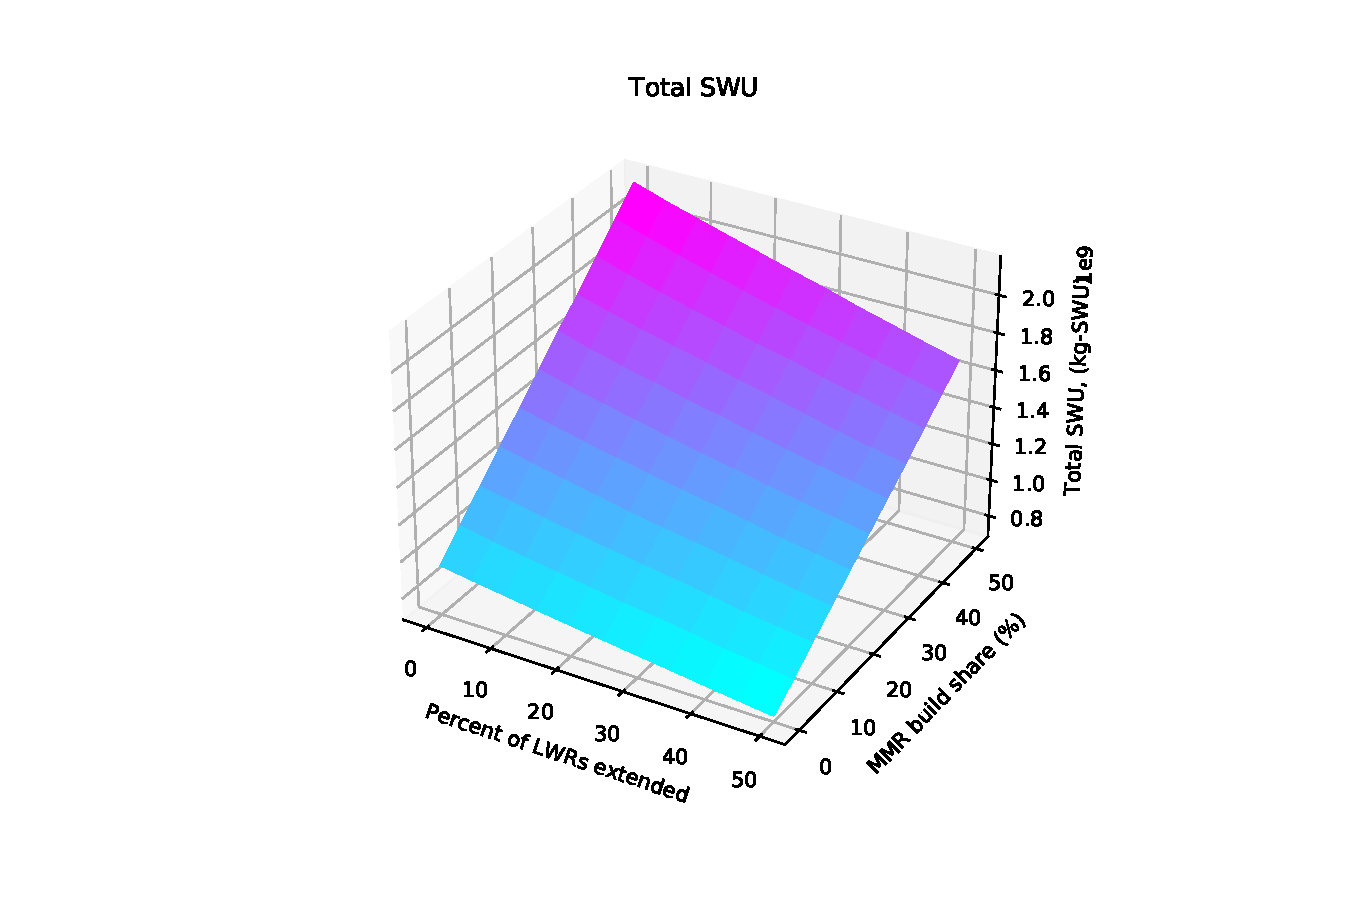
\includegraphics[width=\textwidth, trim=120 0 120 30, clip]{lwr_mmr_share_swu.pdf}
        \caption{Effect on total SWU capacity.}
        \label{fig:lwr_mmr_share_swu}
    \end{subfigure}
    \hfill
    \begin{subfigure}[h!]{0.48\textwidth}
        \centering
        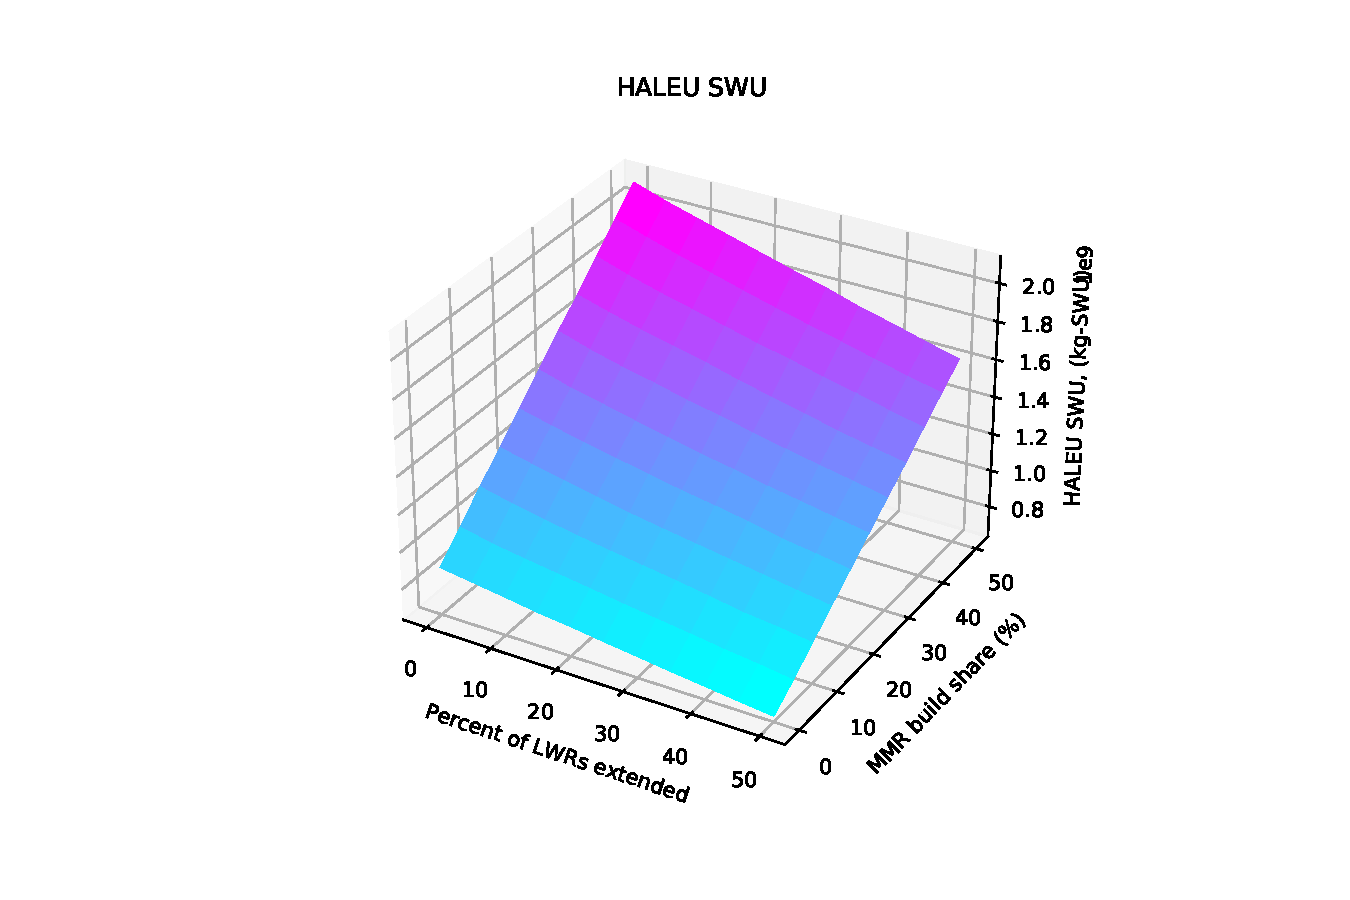
\includegraphics[width=\textwidth, trim=120 0 120 30, clip]{lwr_mmr_share_haleu_swu.pdf}
        \caption{Effect on HALEU SWU capacity.}
        \label{fig:lwr_mmr_share_haleu_swu}
    \end{subfigure}

    \begin{subfigure}[h!]{0.48\textwidth}
        \centering
        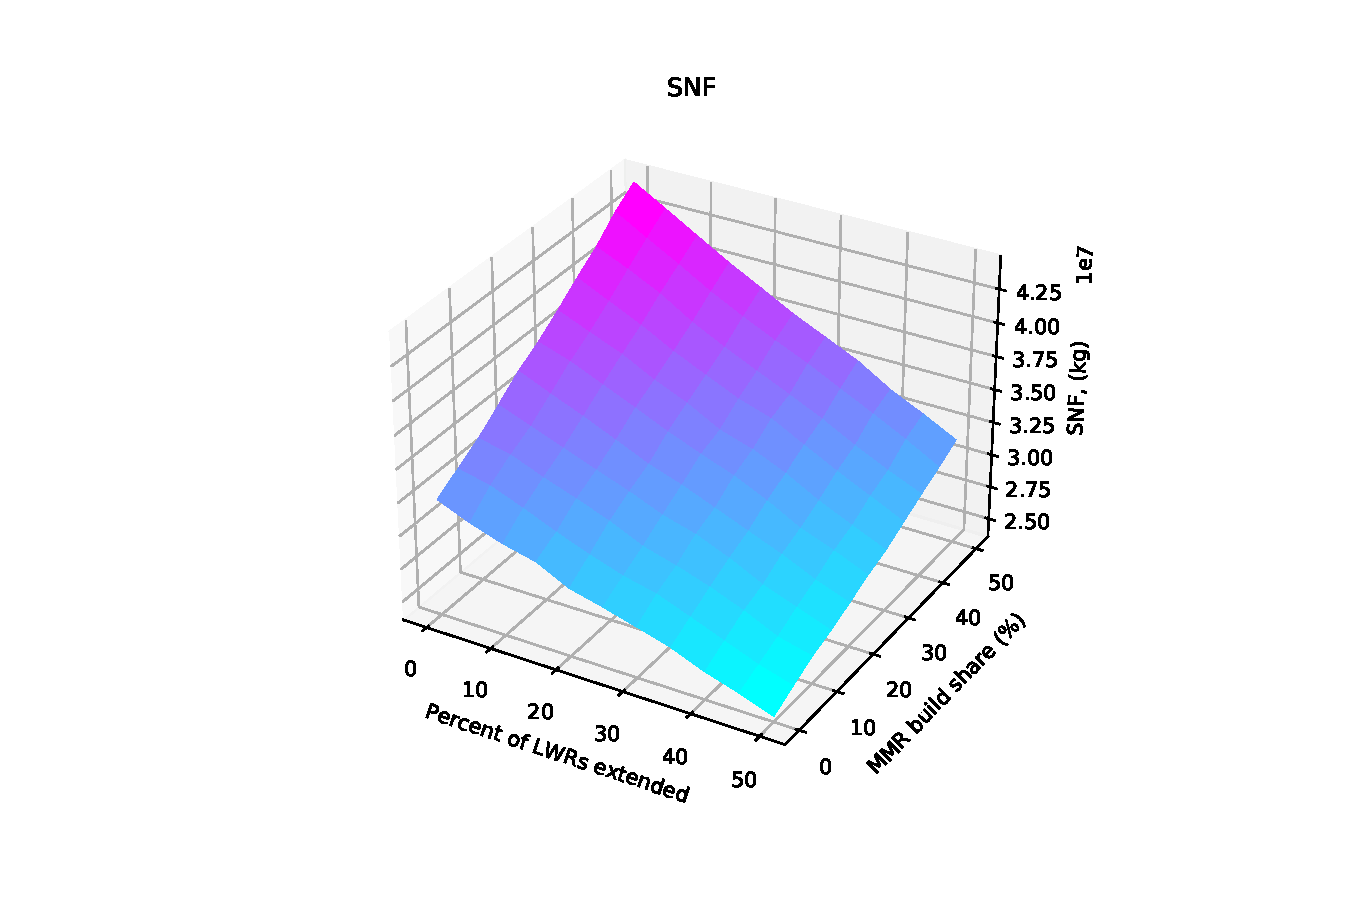
\includegraphics[width=\textwidth, trim=120 0 120 30, clip]{lwr_mmr_share_waste.pdf}
        \caption{Effect on waste mass discharged.}
        \label{fig:lwr_mmr_share_waste}
    \end{subfigure}
    \hfill
    \begin{subfigure}[h!]{0.48\textwidth}
        \centering
        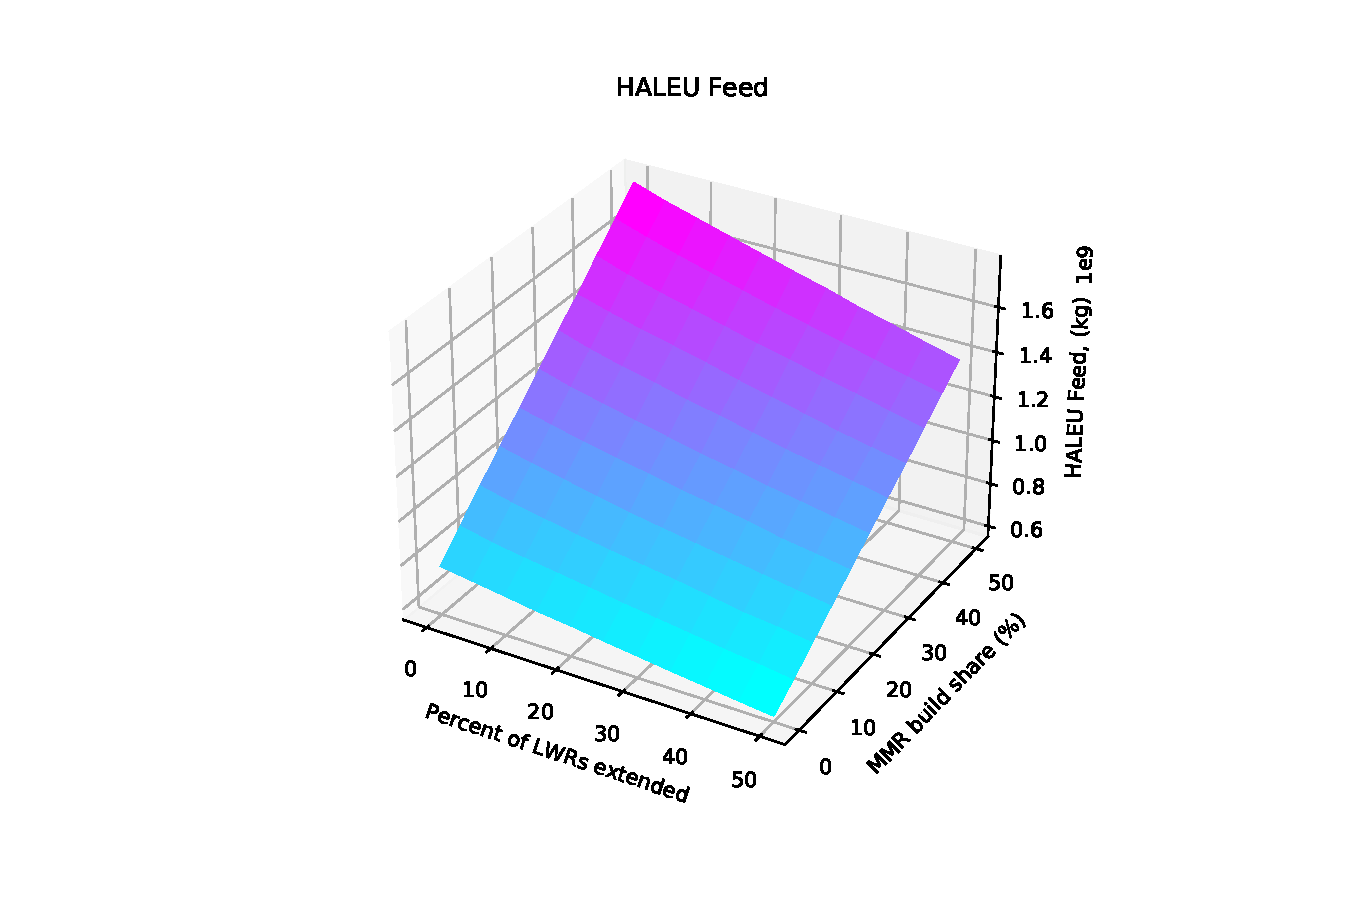
\includegraphics[width=\textwidth, trim=120 0 120 30, clip]{lwr_mmr_share_feed.pdf}
        \caption{Effect on HALEU feed.}
        \label{fig:lwr_mmr_share_feed}
    \end{subfigure}
    \caption{(cont.) Change in metrics resulting from variations in the 
    LWR lifetimes and MMR build share.}
    \label{fig:lwr_mmr_share}
\end{figure}

Figure \ref{fig:lwr_voygr_share} shows the effects of varying the 
percent of \glspl{LWR} operating for 80 years and the VOYGR build share
on the total \gls{SWU} capacity, \gls{HALEU} \gls{SWU} capacity, 
\gls{UNF} mass, and feed mass to produce \gls{HALEU}. The total 
\gls{SWU} capacity, \gls{HALEU} \gls{SWU}, and feed mass exhibit the same 
trend of decreasing with increased \gls{LWR} percent. The \gls{HALEU} 
\gls{SWU} and feed mass decrease with increase VOYGR build share, 
while the total \gls{SWU} capacity is constant. The \gls{UNF} mass 
also decreases with increasing \gls{LWR} percent, but increases with 
the VOYGR build share. 

\begin{figure}   
    \begin{subfigure}[h!]{0.48\textwidth}
        \centering
        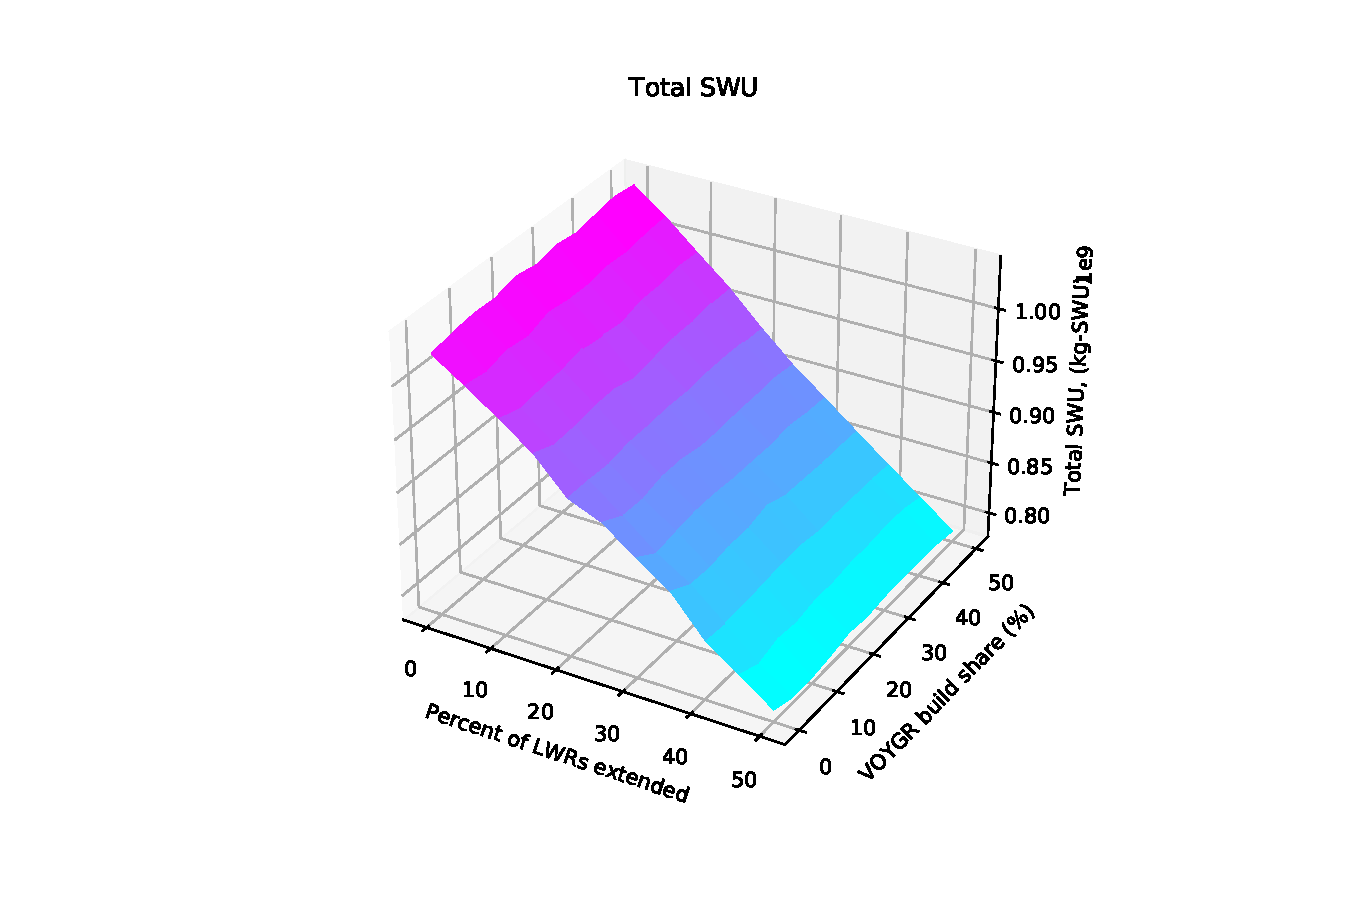
\includegraphics[width=\textwidth, trim=120 0 120 30, clip]{lwr_voygr_share_swu.pdf}
        \caption{Effect on total SWU capacity.}
        \label{fig:lwr_voygr_share_swu}
    \end{subfigure}
    \hfill
    \begin{subfigure}[h!]{0.48\textwidth}
        \centering
        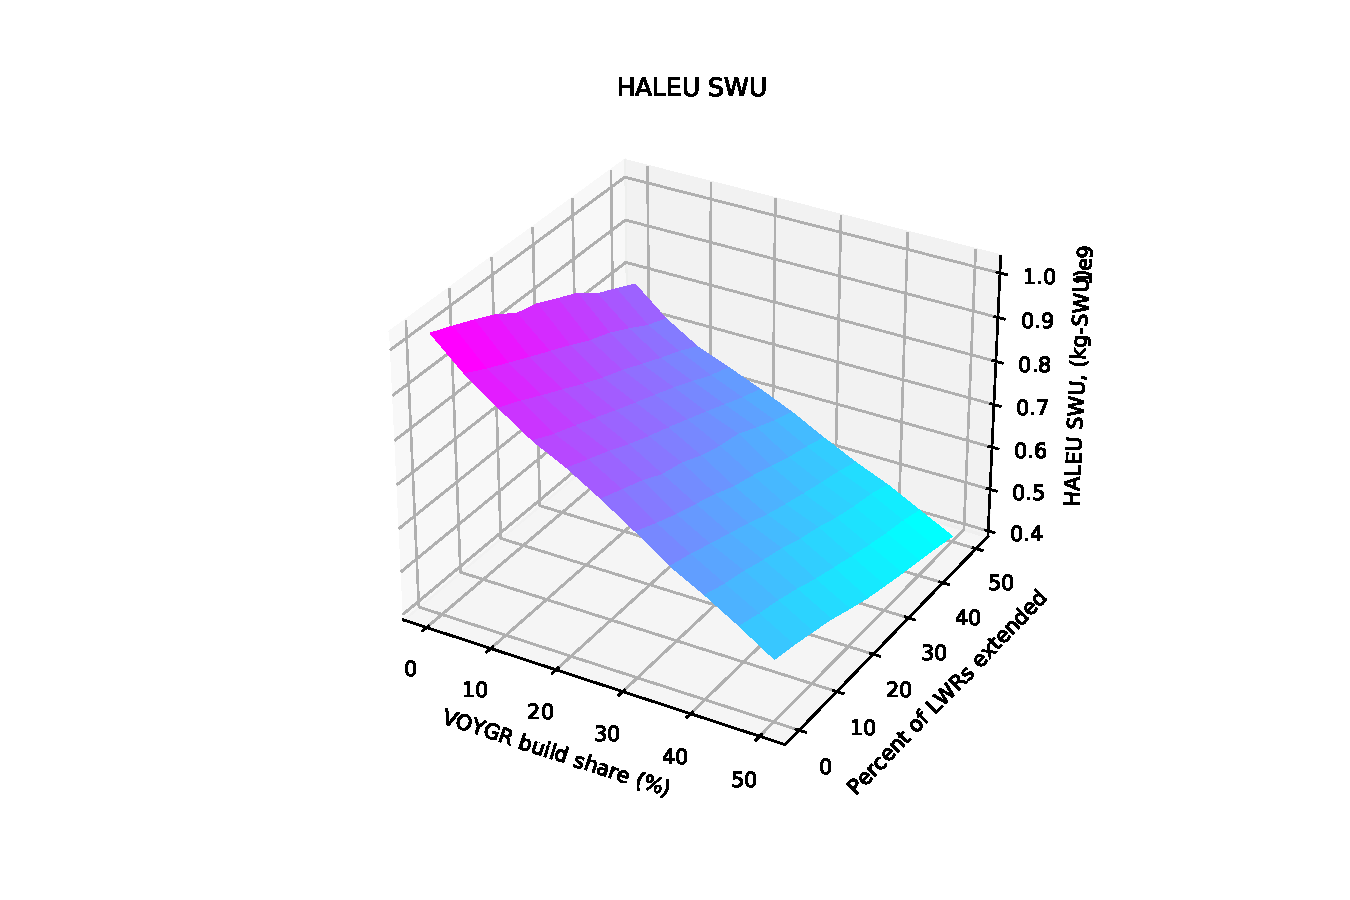
\includegraphics[width=\textwidth, trim=120 0 120 30, clip]{lwr_voygr_share_haleu_swu.pdf}
        \caption{Effect on HALEU SWU capacity.}
        \label{fig:lwr_voygr_share_haleu_swu}
    \end{subfigure}   
    \begin{subfigure}[h!]{0.48\textwidth}
        \centering
        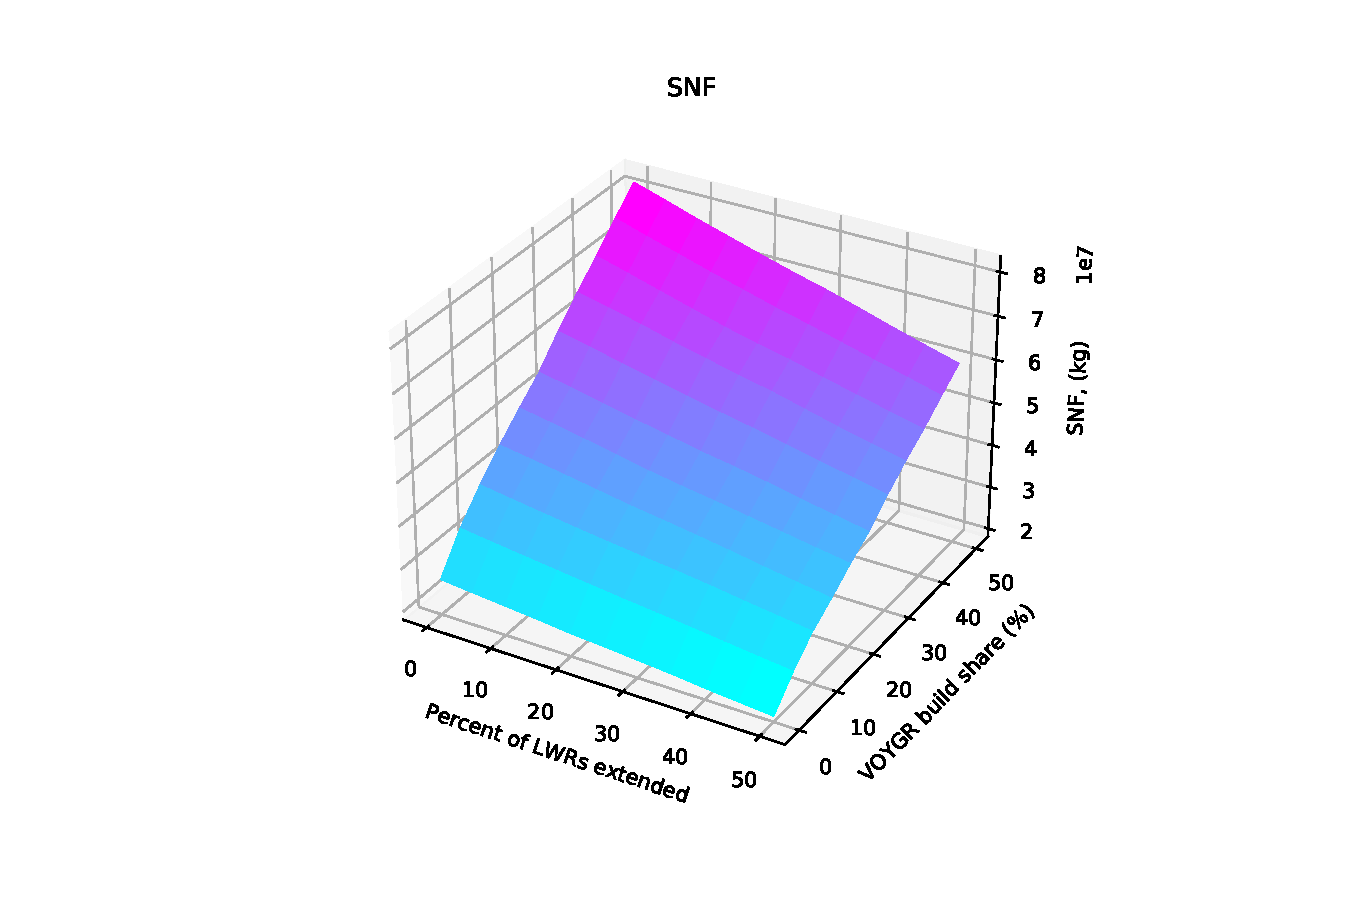
\includegraphics[width=\textwidth, trim=120 0 120 30, clip]{lwr_voygr_share_waste.pdf}
        \caption{Effect on waste mass discharged.}
        \label{fig:lwr_voygr_share_waste}
    \end{subfigure}
    \hfill
    \begin{subfigure}[h!]{0.48\textwidth}
        \centering
        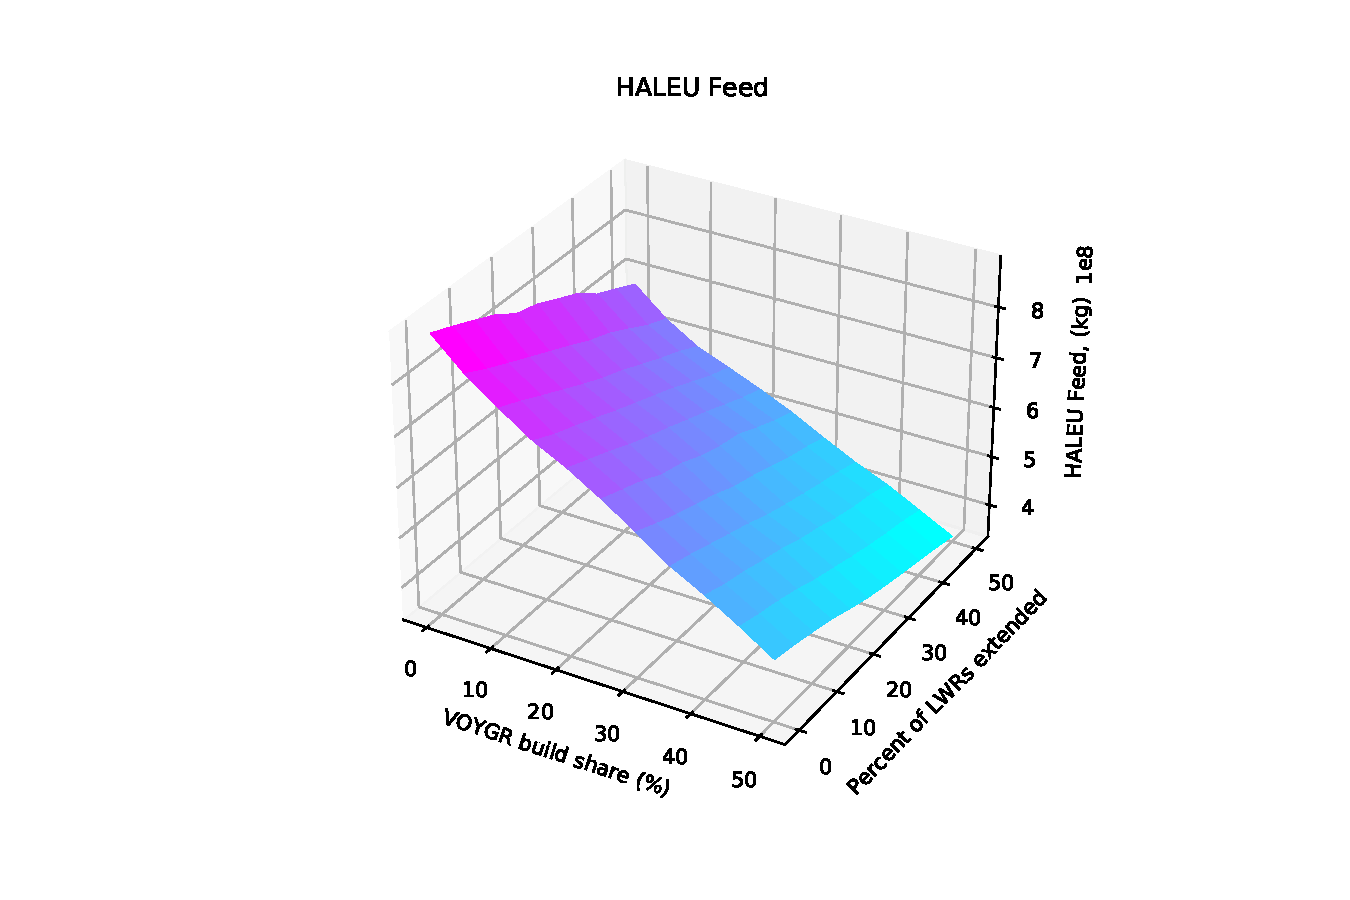
\includegraphics[width=\textwidth, trim=120 0 120 30, clip]{lwr_voygr_share_feed.pdf}
        \caption{Effect on HALEU feed.}
        \label{fig:lwr_voygr_share_feed}
    \end{subfigure}
    \caption{Change in metrics resulting from variations in the 
    LWR lifetimes and VOYGR build share.}
    \label{fig:lwr_voygr_share}
\end{figure}

Figure \ref{fig:lwr_xe100_burnup} shows the effects of varying the 
\gls{LWR} lifetime extension percent and the Xe-100 discharge 
burnup. All of the output metrics exhibit the same trends as these 
parameters are varied, which is consistent with these parameters having 
the same effect on the metrics in the the \gls{OAT} analysis. The metrics 
decrease with increasing 
Xe-100 discharge burnup and increasing number of \glspl{LWR} that 
receive lifetime extensions. The effect of the \gls{LWR} lifetime 
extensions diminishes as the Xe-100 burnup increases, indicating that 
the Xe-100 discharge burnup has a greater influence on the metrics of 
this transition. This result is consistent with most of the advanced 
reactors deployed in this work being Xe-100s and the global analysis 
performed, showing that the Xe-100 discharge burnup consistently had one of 
the highest Sobol' indices. 


\begin{figure}
    \begin{subfigure}[h!]{0.48\textwidth}
        \centering
        \includegraphics[width=\textwidth, trim=120 0 120 30, clip]{lwr_xe100_burnup_enr_u.pdf}
        \caption{Effect on total fuel mass.}
        \label{fig:lwr_xe100_burnup_enr_u}
    \end{subfigure}
    \hfill
    \begin{subfigure}[h!]{0.48\textwidth}
        \centering
        \includegraphics[width=\textwidth, trim=120 0 120 30, clip]{lwr_xe100_burnup_haleu.pdf}
        \caption{Effect on HALEU mass.}
        \label{fig:lwr_xe100_burnup_haleu}
    \end{subfigure}
    
    \begin{subfigure}[h!]{0.48\textwidth}
        \centering
        \includegraphics[width=\textwidth, trim=120 0 120 30, clip]{lwr_xe100_burnup_swu.pdf}
        \caption{Effect on total SWU capacity.}
        \label{fig:lwr_xe100_burnup_swu}
    \end{subfigure}
    \hfill
    \begin{subfigure}[h!]{0.48\textwidth}
        \centering
        \includegraphics[width=\textwidth, trim=120 0 120 30, clip]{lwr_xe100_burnup_haleu_swu.pdf}
        \caption{Effect on HALEU SWU capacity.}
        \label{fig:lwr_xe100_burnup_haleu_swu}
    \end{subfigure}
    \caption{Change in metrics resulting from variations in the 
    LWR lifetimes and the Xe-100 discharge burnup}
\end{figure}

\begin{figure}
    \ContinuedFloat    
    \begin{subfigure}[h!]{0.48\textwidth}
        \centering
        \includegraphics[width=\textwidth, trim=120 0 120 30, clip]{lwr_xe100_burnup_waste.pdf}
        \caption{Effect on waste mass discharged.}
        \label{fig:lwr_xe100_burnup_waste}
    \end{subfigure}
    \hfill
    \begin{subfigure}[h!]{0.48\textwidth}
        \centering
        \includegraphics[width=\textwidth, trim=120 0 120 30, clip]{lwr_xe100_burnup_feed.pdf}
        \caption{Effect on HALEU feed.}
        \label{fig:lwr_xe100_burnup_feed}
    \end{subfigure}
    \caption{(cont.) Change in metrics resulting from variations in the 
    LWR lifetimes and the Xe-100 discharge burnup}
    \label{fig:lwr_xe100_burnup}
\end{figure}

Figure \ref{fig:lwr_mmr_burnup} shows the effects of varying the percent 
of \gls{LWR} operating for 80 years and the \gls{MMR} discharge burnup. 
Varying these parameters has the same effect on all of the metrics: 
increasing these parameters decreases the metrics. The \gls{LWR} lifetime 
has a greater effect on the metrics than the \gls{MMR} burnup because 
\glspl{MMR} supply a small share of the energy demand, compared with 
the other advanced reactors. 
\begin{figure}
    \begin{subfigure}[h!]{0.48\textwidth}
        \centering
        \includegraphics[width=\textwidth, trim=120 0 120 30, clip]{lwr_mmr_burnup_enr_u.pdf}
        \caption{Effect on total fuel mass.}
        \label{fig:lwr_mmr_burnup__enr_u}
    \end{subfigure}
    \hfill
    \begin{subfigure}[h!]{0.48\textwidth}
        \centering
        \includegraphics[width=\textwidth, trim=120 0 120 30, clip]{lwr_mmr_burnup_haleu.pdf}
        \caption{Effect on HALEU mass.}
        \label{fig:lwr_mmr_burnup_haleu}
    \end{subfigure}
    \caption{Change in metrics resulting from variations in the 
    LWR lifetimes and MMR discharge burnup.}
\end{figure}

\begin{figure}
    \ContinuedFloat    
    \begin{subfigure}[h!]{0.48\textwidth}
        \centering
        \includegraphics[width=\textwidth, trim=120 0 120 30, clip]{lwr_mmr_burnup_swu.pdf}
        \caption{Effect on total SWU capacity.}
        \label{fig:lwr_mmr_burnup_swu}
    \end{subfigure}
    \hfill
    \begin{subfigure}[h!]{0.48\textwidth}
        \centering
        \includegraphics[width=\textwidth, trim=120 0 120 30, clip]{lwr_mmr_burnup_haleu_swu.pdf}
        \caption{Effect on HALEU SWU capacity.}
        \label{fig:lwr_mmr_burnup_haleu_swu}
    \end{subfigure}
    
    \begin{subfigure}[h!]{0.48\textwidth}
        \centering
        \includegraphics[width=\textwidth, trim=120 0 120 30, clip]{lwr_mmr_burnup_waste.pdf}
        \caption{Effect on waste mass discharged.}
        \label{fig:lwr_mmr_burnup_waste}
    \end{subfigure}
    \hfill
    \begin{subfigure}[h!]{0.48\textwidth}
        \centering
        \includegraphics[width=\textwidth, trim=120 0 120 30, clip]{lwr_mmr_burnup_feed.pdf}
        \caption{Effect on HALEU feed.}
        \label{fig:lwr_mmr_burnup_feed}
    \end{subfigure}
    \caption{(cont.) Change in metrics resulting from variations in the 
    LWR lifetimes and MMR discharge burnup.}
    \label{fig:lwr_mmr_burnup}
\end{figure}

Figure \ref{fig:mmr_share_xe100_burnup} shows the effects from varying 
the \gls{MMR} build share and the Xe-100 discharge burnup on the 
\gls{HALEU} mass, total \gls{SWU} capacity, \gls{HALEU} \gls{SWU} 
capacity, \gls{UNF} mass discharged, and the feed mass to produce \gls{HALEU}. 
The effects on each of these metrics are consistent with the effects on 
the total enriched uranium mass, presented in Section \ref{sec:synergistic}.
Increasing both of the parameters has contradictory effects. Increasing the 
Xe-100 burnup decreases all of the metrics while increasing the \gls{MMR} 
build share increases all of the metrics. As the \gls{MMR} build share 
increases, the Xe-100 burnup has a smaller impact on the metrics because 
fewer of the advanced reactors deployed are Xe-100s. 


\begin{figure}
    \begin{subfigure}[h!]{0.48\textwidth}
        \centering
        \includegraphics[width=\textwidth, trim=120 0 120 30, clip]{mmr_share_xe100_burnup_haleu.pdf}
        \caption{Effect on HALEU mass.}
        \label{fig:mmr_share_xe100_burnup_haleu}
    \end{subfigure}
    \hfill 
    \begin{subfigure}[h!]{0.48\textwidth}
        \centering
        \includegraphics[width=\textwidth, trim=120 0 120 30, clip]{mmr_share_xe100_burnup_swu.pdf}
        \caption{Effect on total SWU capacity.}
        \label{fig:mmr_share_xe100_burnup_swu}
    \end{subfigure}
    \hfill
    \begin{subfigure}[h!]{0.48\textwidth}
        \centering
        \includegraphics[width=\textwidth, trim=120 0 120 30, clip]{mmr_share_xe100_burnup_haleu_swu.pdf}
        \caption{Effect on HALEU SWU capacity.}
        \label{fig:mmr_share_xe100_burnup_haleu_swu}
    \end{subfigure}
    \hfill
    \begin{subfigure}[h!]{0.48\textwidth}
        \centering
        \includegraphics[width=\textwidth, trim=120 0 120 30, clip]{mmr_share_xe100_burnup_waste.pdf}
        \caption{Effect on waste mass discharged.}
        \label{fig:mmr_share_xe100_burnup_waste}
    \end{subfigure}
    \caption{Change in metrics resulting from variations in the 
    MMR build share and Xe-100 discharge burnup.}
\end{figure}

\begin{figure}
    \ContinuedFloat
    \begin{subfigure}[h!]{0.48\textwidth}
        \centering
        \includegraphics[width=\textwidth, trim=120 0 120 30, clip]{mmr_share_xe100_burnup_feed.pdf}
        \caption{Effect on HALEU feed.}
        \label{fig:mmr_share_xe100_burnup_feed}
    \end{subfigure}
    \caption{(cont.) Change in metrics resulting from variations in the 
    MMR build share and Xe-100 discharge burnup.}
    \label{fig:mmr_share_xe100_burnup}
\end{figure}

Figure \ref{fig:mmr_share_mmr_burnup} shows the effects of varying 
the \gls{MMR} share and \gls{MMR} burnup on all of the metrics. All of 
the metrics exhibit the same trends as each parameter is varied: the 
metrics decrease with increasing \gls{MMR} burnup and increase 
with increasing \gls{MMR} build share. This trends are a result of 
less fuel and materials produce the fuel as the \gls{MMR} burnup increases, 
but the \gls{MMR} requiring more materials than Xe-100 to meet the same 
energy demand. These two parameters have a 
compounding effect, such that as the \gls{MMR} build share increases 
the variations in the burnup have a greater impact on the metrics because 
\glspl{MMR} comprise more of the advanced reactor fleet. All of the metrics 
are at a minimum when the \gls{MMR} build share is 0\%, independent of 
the \gls{MMR} burnup. This result is because if there are no \glspl{MMR} 
deployed in the transition, then the discharge burnup of the fuel that 
goes into these reactors has no effect on the transition. 


\begin{figure}
    \begin{subfigure}[h!]{0.48\textwidth}
        \centering
        \includegraphics[width=\textwidth, trim=120 0 120 30, clip]{mmr_share_mmr_burnup_enr_u.pdf}
        \caption{Effect on total fuel mass.}
        \label{fig:mmr_share_mmr_burnup_enr_u}
    \end{subfigure}
    \hfill
    \begin{subfigure}[h!]{0.48\textwidth}
        \centering
        \includegraphics[width=\textwidth, trim=120 0 120 30, clip]{mmr_share_mmr_burnup_haleu.pdf}
        \caption{Effect on HALEU mass.}
        \label{fig:mmr_share_mmr_burnup_haleu}
    \end{subfigure}
    \caption{Change in metrics resulting from variations in the 
    MMR build share and MMR discharge burnup.}
\end{figure}

\begin{figure}
    \ContinuedFloat    
    \begin{subfigure}[h!]{0.48\textwidth}
        \centering
        \includegraphics[width=\textwidth, trim=120 0 120 30, clip]{mmr_share_mmr_burnup_swu.pdf}
        \caption{Effect on total SWU capacity.}
        \label{fig:mmr_share_mmr_burnup_swu}
    \end{subfigure}
    \hfill
    \begin{subfigure}[h!]{0.48\textwidth}
        \centering
        \includegraphics[width=\textwidth, trim=120 0 120 30, clip]{mmr_share_mmr_burnup_haleu_swu.pdf}
        \caption{Effect on HALEU SWU capacity.}
        \label{fig:mmr_share_mmr_burnup_haleu_swu}
    \end{subfigure}
    
    \begin{subfigure}[h!]{0.48\textwidth}
        \centering
        \includegraphics[width=\textwidth, trim=120 0 120 30, clip]{mmr_share_mmr_burnup_waste.pdf}
        \caption{Effect on waste mass discharged.}
        \label{fig:mmr_share_mmr_burnup_waste}
    \end{subfigure}
    \hfill
    \begin{subfigure}[h!]{0.48\textwidth}
        \centering
        \includegraphics[width=\textwidth, trim=120 0 120 30, clip]{mmr_share_mmr_burnup_feed.pdf}
        \caption{Effect on HALEU feed.}
        \label{fig:mmr_share_mmr_burnup_feed}
    \end{subfigure}
    \caption{(cont.) Change in metrics resulting from variations in the 
    MMR build share and MMR discharge burnup.}
    \label{fig:mmr_share_mmr_burnup}
\end{figure}

Figure \ref{fig:xe100_share_xe100_burnup} shows the effects of varying 
the Xe-100 build share and Xe-100 discharge burnup on total \gls{SWU}
capacity, \gls{HALEU} \gls{SWU} capacity, \gls{UNF} mass discharged, and
the feed mass to produce \gls{HALEU}. The \gls{UNF} exhibits a different 
trend than the other three metrics. As the Xe-100 build share and 
burnup increase the \gls{UNF} mass decreases. The other metrics generally
increase with increasing Xe-100 build share and decreasing burnup. 
As identified in the \gls{OAT} analysis, the effects in the metrics from 
varying the Xe-100 build share is a result of design and material 
requirement differences between the Xe-100 and VOYGR. Therefore, the 
different trends in each of the metrics as the Xe-100 build share increases 
is a result of the difference in the two reactor designs. 
In each of 
the metrics, the impact of the Xe-100 burnup increases as the 
Xe-100 build share increases because Xe-100s comprise more of 
the advanced reactor fleet. Additionally, the metrics have a constant value 
as a function of Xe-100 burnup when the build share is 0\% because none 
of the advanced reactors deployed are Xe-100s. 

The \gls{OAT} showed that as the Xe-100 build share increases, the 
total \gls{SWU} capacity remained constant for a given burnup because 
of the trade-off in enrichment level and mass of fuel between the Xe-100 
and VOYGR. The results of the synergistic analysis show that this 
metric only remains relatively constant for high burnup values. At 
low burnup values (below about 140 MWd/kgU), the Xe-100 requires more 
fuel mass than the VOYGR, which means that more \gls{SWU} capacity 
is needed to fuel the reactors. 

\begin{figure}    
    \begin{subfigure}[h!]{0.48\textwidth}
        \centering
        \includegraphics[width=\textwidth, trim=120 0 120 30, clip]{xe100_share_xe100_burnup_swu.pdf}
        \caption{Effect on total SWU capacity.}
        \label{fig:xe100_share_xe100_burnup_swu}
    \end{subfigure}
    \hfill
    \begin{subfigure}[h!]{0.48\textwidth}
        \centering
        \includegraphics[width=\textwidth, trim=120 0 120 30, clip]{xe100_share_xe100_burnup_haleu_swu.pdf}
        \caption{Effect on HALEU SWU capacity.}
        \label{fig:xe100_share_xe100_burnup_haleu_swu}
    \end{subfigure}
    
    \begin{subfigure}[h!]{0.48\textwidth}
        \centering
        \includegraphics[width=\textwidth, trim=120 0 120 30, clip]{xe100_share_xe100_burnup_waste.pdf}
        \caption{Effect on waste mass discharged.}
        \label{fig:xe100_share_xe100_burnup_waste}
    \end{subfigure}
    \hfill
    \begin{subfigure}[h!]{0.48\textwidth}
        \centering
        \includegraphics[width=\textwidth, trim=120 0 120 30, clip]{xe100_share_xe100_burnup_feed.pdf}
        \caption{Effect on HALEU feed.}
        \label{fig:xe100_share_xe100_burnup_feed}
    \end{subfigure}
    \caption{Change in metrics resulting from variations in the 
    Xe-100 build share and Xe-100 discharge burnup.}
    \label{fig:xe100_share_xe100_burnup}
\end{figure}

Figure \ref{fig:xe100_share_mmr_burnup} shows the effects of varying the 
Xe-100 build share and the \gls{MMR} burnup on each of the metrics. 
The total fuel mass and \gls{UNF} mass decrease with increasing 
Xe-100 build share and are affected little by the \gls{MMR} burnup. The
\gls{HALEU} mass, \gls{HALEU} \gls{SWU}, and feed mass to produce 
\gls{HALEU} the Xe-100 build share  increase with increasing Xe-100 
build share and are affected little by the \gls{MMR} burnup. The total 
\gls{SWU} capacity decreases with increasing \gls{MMR} burnup and is 
affected little by the Xe-100 build share. All of the metrics are only 
strongly influenced by one of the parameters varied, which indicates that 
these two parameters do not interact. Variations in the Xe-100 build 
share primarily impacts the number of Xe-100s and VOYGRs built, as shown 
in the \gls{OAT} analysis. Because this parameter does not greatly affect 
the number of \glspl{MMR} deployed, these two parameters do not have any 
combined effects on the metrics. The total \gls{SWU} capacity is most affected 
by the \gls{MMR} burnup because the Xe-100 build share primarily 
affects the deployment of Xe-100s and VOYGRs, and these two reactors 
require similar \gls{SWU} capacity. Therefore, the changes in fuel 
requirements and \gls{SWU} capacity from varying the \gls{MMR} burnup 
is greater than the change in the change in \gls{SWU} capacity from 
varying the Xe-100 build share. 
\begin{figure}
    \begin{subfigure}[h!]{0.48\textwidth}
        \centering
        \includegraphics[width=\textwidth, trim=120 0 120 30, clip]{xe100_share_mmr_burnup_enr_u.pdf}
        \caption{Effect on total fuel mass.}
        \label{fig:xe100_share_mmr_burnup_enr_u}
    \end{subfigure}
    \hfill
    \begin{subfigure}[h!]{0.48\textwidth}
        \centering
        \includegraphics[width=\textwidth, trim=120 0 120 30, clip]{xe100_share_mmr_burnup_haleu.pdf}
        \caption{Effect on HALEU mass.}
        \label{fig:xe100_share_mmr_burnup_haleu}
    \end{subfigure}
    
    \begin{subfigure}[h!]{0.48\textwidth}
        \centering
        \includegraphics[width=\textwidth, trim=120 0 120 30, clip]{xe100_share_mmr_burnup_swu.pdf}
        \caption{Effect on total SWU capacity.}
        \label{fig:xe100_share_mmr_burnup_swu}
    \end{subfigure}
    \hfill
    \begin{subfigure}[h!]{0.48\textwidth}
        \centering
        \includegraphics[width=\textwidth, trim=120 0 120 30, clip]{xe100_share_mmr_burnup_haleu_swu.pdf}
        \caption{Effect on HALEU SWU capacity.}
        \label{fig:xe100_share_mmr_burnup_haleu_swu}
    \end{subfigure}   
    \caption{Change in metrics resulting from variations in the 
    Xe-100 build share and MMR discharge burnup} 
\end{figure}

\begin{figure}
    \ContinuedFloat    
    \begin{subfigure}[h!]{0.48\textwidth}
        \centering
        \includegraphics[width=\textwidth, trim=120 0 120 30, clip]{xe100_share_mmr_burnup_waste.pdf}
        \caption{Effect on waste mass discharged.}
        \label{fig:xe100_share_mmr_burnup_waste}
    \end{subfigure}
    \hfill
    \begin{subfigure}[h!]{0.48\textwidth}
        \centering
        \includegraphics[width=\textwidth, trim=120 0 120 30, clip]{xe100_share_mmr_burnup_feed.pdf}
        \caption{Effect on HALEU feed.}
        \label{fig:xe100_share_mmr_burnup_feed}
    \end{subfigure}
    \caption{(cont.) Change in metrics resulting from variations in the 
    Xe-100 build share and MMR discharge burnup}
    \label{fig:xe100_share_mmr_burnup}
\end{figure}

Figure \ref{fig:voygr_share_mmr_burnup} shows the results of varying the 
VOYGR build share and the Xe-100 burnup on all of the metrics. All six 
metrics decrease as a function of the Xe-100 burnup. The total fuel 
mass and \gls{UNF} generally decrease with the VOYGR build share while 
the \gls{HALEU}-related metrics and total \gls{SWU} capacity decrease 
with increasing build share. The results indicate that there is interaction 
between these two parameters. As the VOYGR build share increases, the number 
of Xe-100s deployed decreases. This effect is the opposite of the result of 
increasing the Xe-100 build share. Therefore, the VOYGR build share and 
Xe-100 burnup interact in opposite ways as the Xe-100 build share and the 
Xe-100 burnup. As the VOYGR build share increases, the Xe-100 burnup has less impact on the 
metrics. Additionally, as the Xe-100 burnup increases, the VOYGR 
build share has less impact on the metrics. 

\begin{figure}
    \begin{subfigure}[h!]{0.48\textwidth}
        \centering
        \includegraphics[width=\textwidth, trim=120 0 120 30, clip]{voygr_share_xe100_burnup_enr_u.pdf}
        \caption{Effect on total fuel mass.}
        \label{fig:voygr_share_xe100_burnup_enr_u}
    \end{subfigure}
    \hfill
    \begin{subfigure}[h!]{0.48\textwidth}
        \centering
        \includegraphics[width=\textwidth, trim=120 0 120 30, clip]{voygr_share_xe100_burnup_haleu.pdf}
        \caption{Effect on HALEU mass.}
        \label{fig:voygr_share_xe100_burnup_haleu}
    \end{subfigure}  
    \begin{subfigure}[h!]{0.48\textwidth}
        \centering
        \includegraphics[width=\textwidth, trim=120 0 120 30, clip]{voygr_share_xe100_burnup_swu.pdf}
        \caption{Effect on total SWU capacity.}
        \label{fig:voygr_share_xe100_burnup_swu}
    \end{subfigure}
    \hfill
    \begin{subfigure}[h!]{0.48\textwidth}
        \centering
        \includegraphics[width=\textwidth, trim=120 0 120 30, clip]{voygr_share_xe100_burnup_haleu_swu.pdf}
        \caption{Effect on HALEU SWU capacity.}
        \label{fig:voygr_share_xe100_burnup_haleu_swu}
    \end{subfigure}
    \caption{Change in metrics resulting from variations in the 
    VOYGR build share and Xe-100 discharge burnup.}
\end{figure}

\begin{figure}
    \ContinuedFloat      
    \begin{subfigure}[h!]{0.48\textwidth}
        \centering
        \includegraphics[width=\textwidth, trim=120 0 120 30, clip]{voygr_share_xe100_burnup_waste.pdf}
        \caption{Effect on waste mass discharged.}
        \label{fig:voygr_share_xe100_burnup_waste}
    \end{subfigure}
    \hfill
    \begin{subfigure}[h!]{0.48\textwidth}
        \centering
        \includegraphics[width=\textwidth, trim=120 0 120 30, clip]{voygr_share_xe100_burnup_feed.pdf}
        \caption{Effect on HALEU feed.}
        \label{fig:voygr_share_xe100_burnup_feed}
    \end{subfigure}
    \caption{(cont.) Change in metrics resulting from variations in the 
    VOYGR build share and Xe-100 discharge burnup.}
    \label{fig:voygr_share_xe100_burnup}
\end{figure}

Figure \ref{fig:voygr_share_mmr_burnup} shows the effects of varying 
the VOYGR build share and \gls{MMR} burnup on all of the metrics. The 
results of varying these two parameters is similar, but opposite in 
direction, to the results of varying the Xe-100 build share and 
\gls{MMR} burnup. The total fuel mass ans \gls{UNF} mass increase 
with increasing VOYGR build share and are not impacted greatly by the 
\gls{MMR} burnup. The \gls{HALEU}-related metrics decrease with 
increasing VOYGR build share and are not greatly affected by the 
\gls{MMR} burnup. The total \gls{SWU} capacity decreases with increasing 
\gls{MMR} burnup and is not greatly affected by the VOYGR build share. 
These results identify that these two parameters do not 
interact with each other. The VOYGR build share affects the number of 
VOYGRs and Xe-100s deployed, while the \gls{MMR} burnup affects the 
fuel requirements of the the \glspl{MMR} that are deployed. 

\begin{figure}
    \begin{subfigure}[h!]{0.48\textwidth}
        \centering
        \includegraphics[width=\textwidth, trim=120 0 120 30, clip]{voygr_share_mmr_burnup_enr_u.pdf}
        \caption{Effect on total fuel mass.}
        \label{fig:voygr_share_mmr_burnupenr_u}
    \end{subfigure}
    \hfill
    \begin{subfigure}[h!]{0.48\textwidth}
        \centering
        \includegraphics[width=\textwidth, trim=120 0 120 30, clip]{voygr_share_mmr_burnup_haleu.pdf}
        \caption{Effect on HALEU mass.}
        \label{fig:voygr_share_mmr_burnup_haleu}
    \end{subfigure}
    \caption{Change in metrics resulting from variations in the 
    VOYGR build share and MMR discharge burnup.}
\end{figure}

\begin{figure}
    \ContinuedFloat  
    
    \begin{subfigure}[h!]{0.48\textwidth}
        \centering
        \includegraphics[width=\textwidth, trim=120 0 120 30, clip]{voygr_share_mmr_burnup_swu.pdf}
        \caption{Effect on total SWU capacity.}
        \label{fig:voygr_share_mmr_burnup_swu}
    \end{subfigure}
    \hfill
    \begin{subfigure}[h!]{0.48\textwidth}
        \centering
        \includegraphics[width=\textwidth, trim=120 0 120 30, clip]{voygr_share_mmr_burnup_haleu_swu.pdf}
        \caption{Effect on HALEU SWU capacity.}
        \label{fig:voygr_share_mmr_burnup_haleu_swu}
    \end{subfigure}  
    \begin{subfigure}[h!]{0.48\textwidth}
        \centering
        \includegraphics[width=\textwidth, trim=120 0 120 30, clip]{voygr_share_mmr_burnup_waste.pdf}
        \caption{Effect on waste mass discharged.}
        \label{fig:voygr_share_mmr_burnup_waste}
    \end{subfigure}
    \hfill
    \begin{subfigure}[h!]{0.48\textwidth}
        \centering
        \includegraphics[width=\textwidth, trim=120 0 120 30, clip]{voygr_share_mmr_burnup_feed.pdf}
        \caption{Effect on HALEU feed.}
        \label{fig:voygr_share_mmr_burnup_feed}
    \end{subfigure}
    \caption{(cont.) Change in metrics resulting from variations in the 
    VOYGR build share and MMR discharge burnup.}
    \label{fig:voygr_share_mmr_burnup}
\end{figure}